\documentclass[referee, pdflatex, sn-mathphys-num]{sn-jnl}

\usepackage{hyperref}
\usepackage{geometry} 
\usepackage{subfigure}
\usepackage{graphicx} 
\usepackage{amsmath,amsfonts,amssymb,amsthm,mathtools}
\usepackage{icomma}
\usepackage[english]{babel}
\usepackage{array,tabularx,tabulary,booktabs}
\usepackage{multirow}

\theoremstyle{definition}
\newtheorem*{Def}{Definition}
\theoremstyle{plain}
\newtheorem{Lem}{Lemma}
\newtheorem{Th}{Theorem}
\newtheorem{Prop}{Property}

% article-specific symbols
\newcommand{\delayV}[1]{\overset{\leftarrow}{\mathbf{x}}_{#1}}
\newcommand{\delayM}[1]{\overset{\leftarrow}{\mathbf{X}}_{#1}}

\begin{document}
	
	\title{Tensor decomposition and forecasting for multivariate time series}
	
	\author*[1]{\fnm{Kirill} \sur{Semkin}}\email{kirill.semkin32@mail.ru}
	\author*[2]{\fnm{Vadim} \sur{Strijov}}\email{strijov@ccas.ru}
	
	\affil*[1]{\orgname{Forecsys$^\text{{\footnotesize \textregistered}}$} \orgaddress{\city{Moscow}} \country{Russia}}
	\affil*[2]{\orgname{Forecsys$^\text{{\footnotesize \textregistered}}$} \orgaddress{\city{Moscow}} \country{Russia}}
	
	\keywords{time series, decomposition, forecast, SSA, CPD}
	
	\maketitle
	
	\begin{abstract}
		
		Processing of multidimensional time series is associated with an additional task of determining dependencies between signals. Its inclusion in models boosts the quality of forecasts. On the other hand, taking this dependency into account makes models more complex and less interpretable. The paper proposes a non-parametric method based on tensor data representation and Singular Spectrum Analysis (SSA). It derives a time series decomposition technique and an explicit forecast model. Finally, it applies an elaborated theory to electricity consumption and inertial measurement unit datasets. It compares the obtained quality of forecast with mSSA, VAR, and RNN models.
		
	\end{abstract}
	
	\section{Introduction}\label{Intro}
	
	The main object of the paper is multivariate time series. It is a set of $ m $ series $ \{x_i(t)\}_{i=1}^m $ observed in discrete time $ t \in 1 , \ldots , N $.	We state two problems concerning them. First, to make a \emph{forecast} is to estimate future values $ \{x_i(T)\}_{i=1}^m $ of the series at time $ T > N $. Second, to build an additive \emph{decomposition} is to represent each signal in a set as a sum of several components: $ x_i(t) = c_1(t) + \ldots + c_s(t), \ \forall i \in 1, \ldots , m $.
	
	For the decomposition in a single-variate time series case the papers~\cite{enders2010applied, x11, cleveland90} introduce seasonal-trend-cycle techniques. For the forecast the authors in~\cite{Box_Jenkins_methodology} propose autoregressive methods as well as works~\cite{3b1355aedd1041f1853e609a410576f3, enders2010applied} suggest exponential smoothing, regression models, and neural networks. However, these methods can not be transferred to the multivariate series straightforwardly if they are interdependent. The paper~\cite{Volterra:1928} models the size of prey-and-predator populations as a coupled system of differential equations. The dynamics of one population depends directly on the other's and vice-versa. Therefore the forecast can not be made separately. 
	
	Some methods both take into account multivariate time series interdependence and make the forecast. First, \emph{recurrent neural network} (RNN)~\cite{neco} connects series and their past values through several layers of nonlinear transformations. This information is encapsulated in the hidden state vector at each time step. With that, one is able to forecast future values~\cite{TEALAB2018334}.
	
	Second, the	\emph{vector autoregression} (VAR)~\cite{VAR_model1, doi:10.1080/01621459.1962.10480664} is a linear stochastic model for multivariate series. Denote vector $ \mathbf{x}_t = (x_1(t) \ldots x_m(t))^{\mathsf{T}} $ as a series realizations at time $ t $, their further dynamics
	
	\begin{equation*}
		\mathbf{x}_t = \boldsymbol{\mu} + \sum\limits_{i = 1}^p A_i \mathbf{x}_{t - i} + \mathbf{u}_t.
	\end{equation*}
	
	Here  $ \boldsymbol{\mu} $ is a constant vector, $ A_i $ are $ m \times m $ matrices, $ \mathbf{u}_t $ is a random vector (e.g. white noise $ \text{WN}(t) $). The time series interdependence is defined by $ A_i $ matrices, so each series depends on each other and their past linearly.
	
	The RNN and VAR methods are able to make the forecast, but, firstly, have a large number of learnable and structural parameters. That means their underlying models have an extensive complexity and their architecture needs to be picked over and tuned. Secondly, the methods' structure does not contain an explicit way of building series decomposition.
	
	To rectify the listed disadvantages, we have developed a new method called \emph{tensor SSA} (tSSA). It has only two adjustable parameters. The tSSA extends an SSA method~\cite{ecfb9dc578be43ae9ee8fc88b8ff9151} for the multivariate time series and implies using dynamical systems theory. 
	
	The main task of the paper is to find a shared \emph{phase subspace}~\cite{1572261550523548160, ignatov2016human} for all given time series. This is a low-dimensional linear subspace where all the system's trajectories can be mapped into isomorphically. Finding it enables us to obtain phase representation of observed signals. Fig.~\ref{pic:phase_traj} illustrates this idea. We use a single time series to build phase space and the specific trajectory of the dynamical system that generated the given series. The forecast then is found upon the fact that the continuation of the trajectory lies in the very same phase space. Partitioning basis vectors of this space into several groups builds us the decomposition of the series. The paper develops named conceptions in the next sections.
	
	\begin{figure}[h]
		\centering
		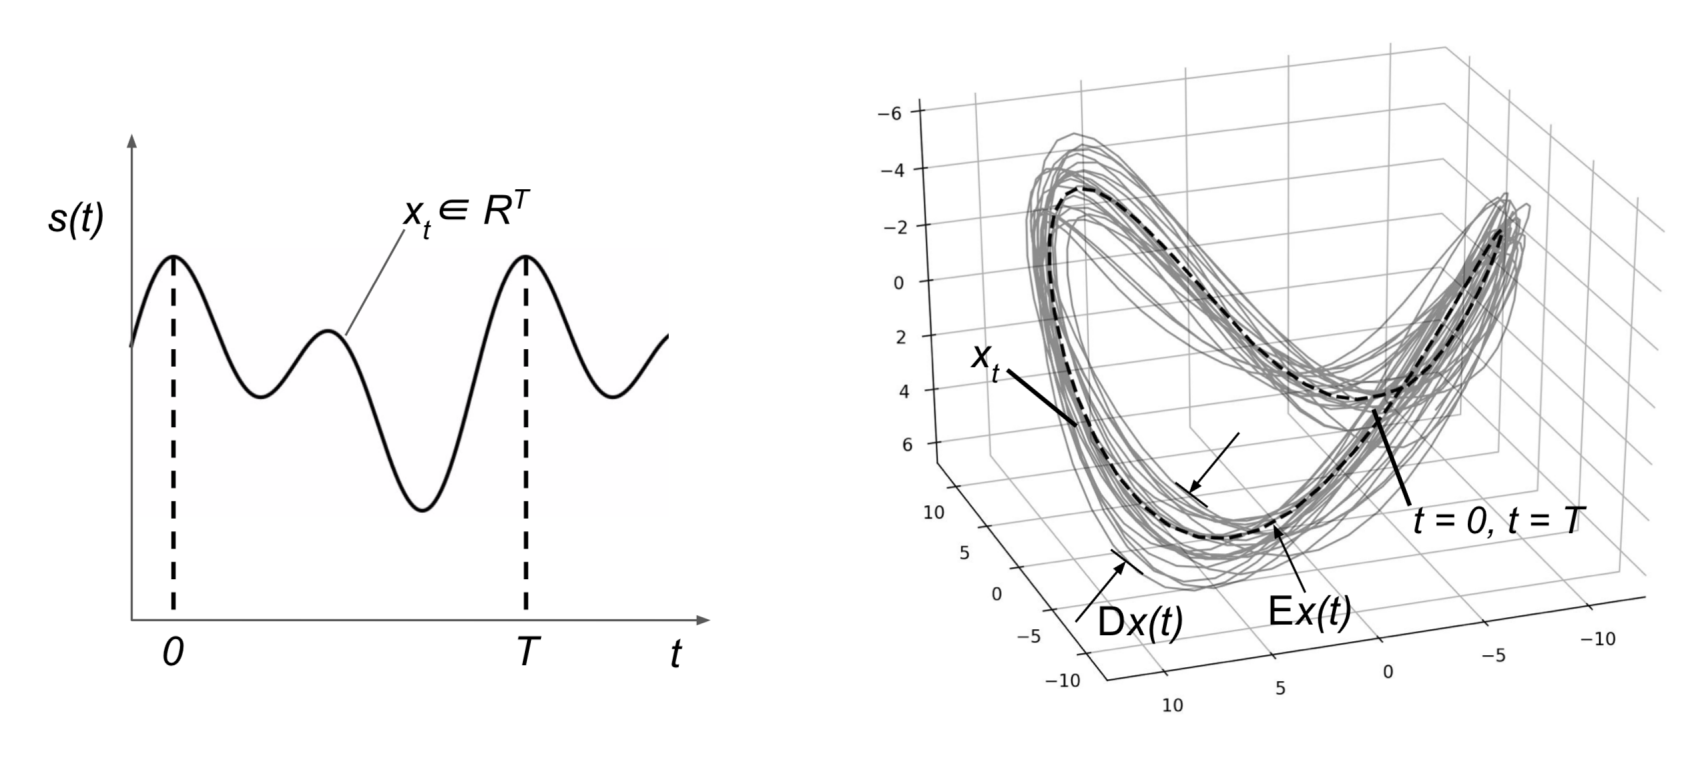
\includegraphics[width=0.9\textwidth, keepaspectratio]{phase_traj.png}
		\caption{Time series's phase trajectory visualization }\label{pic:phase_traj}
	\end{figure}
	
	Our method captures autocorrelation and multilinearity of the time series via tensor data representation. \emph{Canonical polyadic decomposition} (CPD) is used to build the phase space of the series. Another solution is to use matrix data representation and matrix decompositions. Such method is called matrix SSA (mSSA)~\cite{mSSA_overview}. It is the second extension of the SSA method for the forecast and the decomposition of the multivariate time series. The tSSA is compared with the mSSA in the computational experiment section.
	
	The rest of the paper covers the theory and application of our method to real data. Firstly, the dynamical systems model is introduced and the problem of basis search in the phase space is stated and resolved. These results enable us to propose a way of decomposing the series and to make the forecast. Simultaneously, features of obtained solutions are examined and two associated theorems are formulated. Finally, tSSA and mentioned methods are applied to two datasets: electricity consumption and accelerometer/gyroscope observations. We obtain their predictions and additive decompositions. For the latter, a special quality metric is introduced.
	
	\section{Problem statement}\label{sec:problem_statement}
	
	Suppose a \emph{dynamical system} with the phase space $ X $, evolution function $ f $ and the initial state $ \mathbf{y}_0 $. Time space is discrete
	
	\begin{gather*}
		\mathbf{y}(t + 1) = f \bigl( \mathbf{y}(t) \bigr) \ t \in \mathbb{N}, \\
		\mathbf{y}(0) = \mathbf{y}_0 .
	\end{gather*}
	
	Generally, $ X $ is a high-dimensional smooth manifold. Then unknown mapping $ \boldsymbol{\phi}: X \to \mathbb{R}^m $ takes each trajectory point $ \mathbf{y}(t) $ to the multivariate time series realization $ \mathbf{x}_t $
	
	\begin{equation*}
		\boldsymbol{\phi} \bigl( \mathbf{y}(t) \bigr) = \mathbf{x}_t. \text{ Coordinately:} \begin{cases}
			\phi_1 \bigl( \mathbf{y}(t) \bigr) = x_1(t), \\
			\ldots \\
			\phi_m \bigl( \mathbf{y}(t) \bigr) = x_m(t). \\
		\end{cases}
	\end{equation*}
	
	It is assumed that the trajectories $ \mathbf{y}(t) $ belong to the smaller dimension manifold $ M \subset X $. Now the problem is to find an embedding of the $ M $ into $ \mathbb{R}^{L} $ for some $ L $. The second problem is to build a basis in the image of the embedding. Having done that, the initial dynamical system will be described in terms of the standard linear space. The same will hold to all time series $ x_i(t) $.

	\subsection{Single-variate series case}\label{sec:one_series}
	
	The tesnor SSA relies on the SSA method and the Takens theorem~\cite{citeulike:2735031}. The theorem provides the needed embedding in the single-variate series case. Any point $ \mathbf{y}(t) \in M $ corresponds to the following vector:
	
	\begin{equation*}
		\bigl( \, \boldsymbol{\phi} \circ f^{t - L + 1} \bigl( \mathbf{y}(t) \bigr), \ldots , \boldsymbol{\phi} \circ f \bigl( \mathbf{y}(t) \bigr), \boldsymbol{\phi} \circ \mathbf{y}(t) \, \bigr)^{\mathsf{T}} = \bigl( x(t - L + 1), \ldots , x(t-1), x(t) \bigr)^{\mathsf{T}}.
	\end{equation*}
	
	
	It is called a \emph{delay vector} at time $ t $ and is denoted as $ \delayV{t} $. The vector's dimension $ L $ must satisfy condition $ L > 2 \cdot \dim(M) $. The function $ \phi(\cdot) $ must satisfy several regularity conditions. They are omitted here and considered fulfilled.
	
	Now the time series $ x(t) $ with the length $ N $ gives $ N - L + 1 $ delay vectors. Therefore image of the embedding is $ \text{Lin}(\{\delayV{t}\}) $. It represents the phase space of the series and must be low dimensional. This means $ \text{Lin}(\{\delayV{t}\}) \subset \mathbb{R}^L $. Finally, the orthonormal basis is an $ U $-component of the Singular value decomposition (SVD) on a \emph{trajectory matrix} $ \mathbf{H}_x $. It is a stacking of the delay vectors
	
	\[
		\mathbf{H}_x = [ \delayV{1} \ldots  \delayV{N - L + 1}].
	\]
	
	\subsection{Multivariate series case and the tSSA method}\label{sec:tssa_method}
	
	Now there given multivariate time series. Let $ m $ be their number. Hence the $ \boldsymbol{\phi}(\cdot) $ is a multidimensional map. This means that instead of the single delay vector we have $ m $ of them at any time $ t $. Let $ \delayM{t} $ be a matrix $ ( \delayV{1_t} \ldots \delayV{m_t} ) $ called \emph{delay matrix}. Then, the embedding image is a linear span of all $ \delayM{t} $. It is also called the \emph{shared} phase space of the multivariate time series.
	
	\begin{figure}[h]
		\centering
		\subfigure{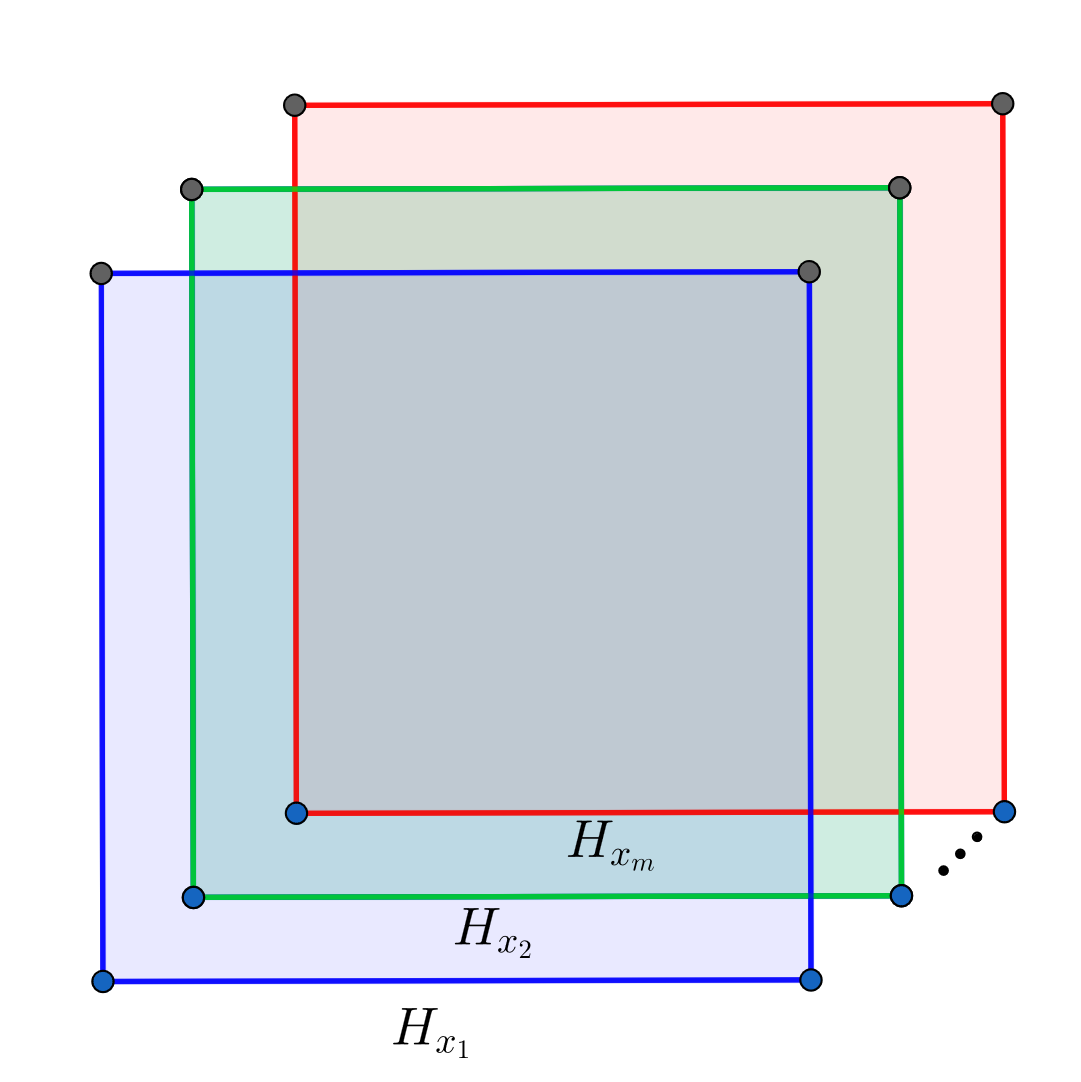
\includegraphics[width=0.4\textwidth, keepaspectratio]{Trajectory_Tensor_1}}
		\subfigure{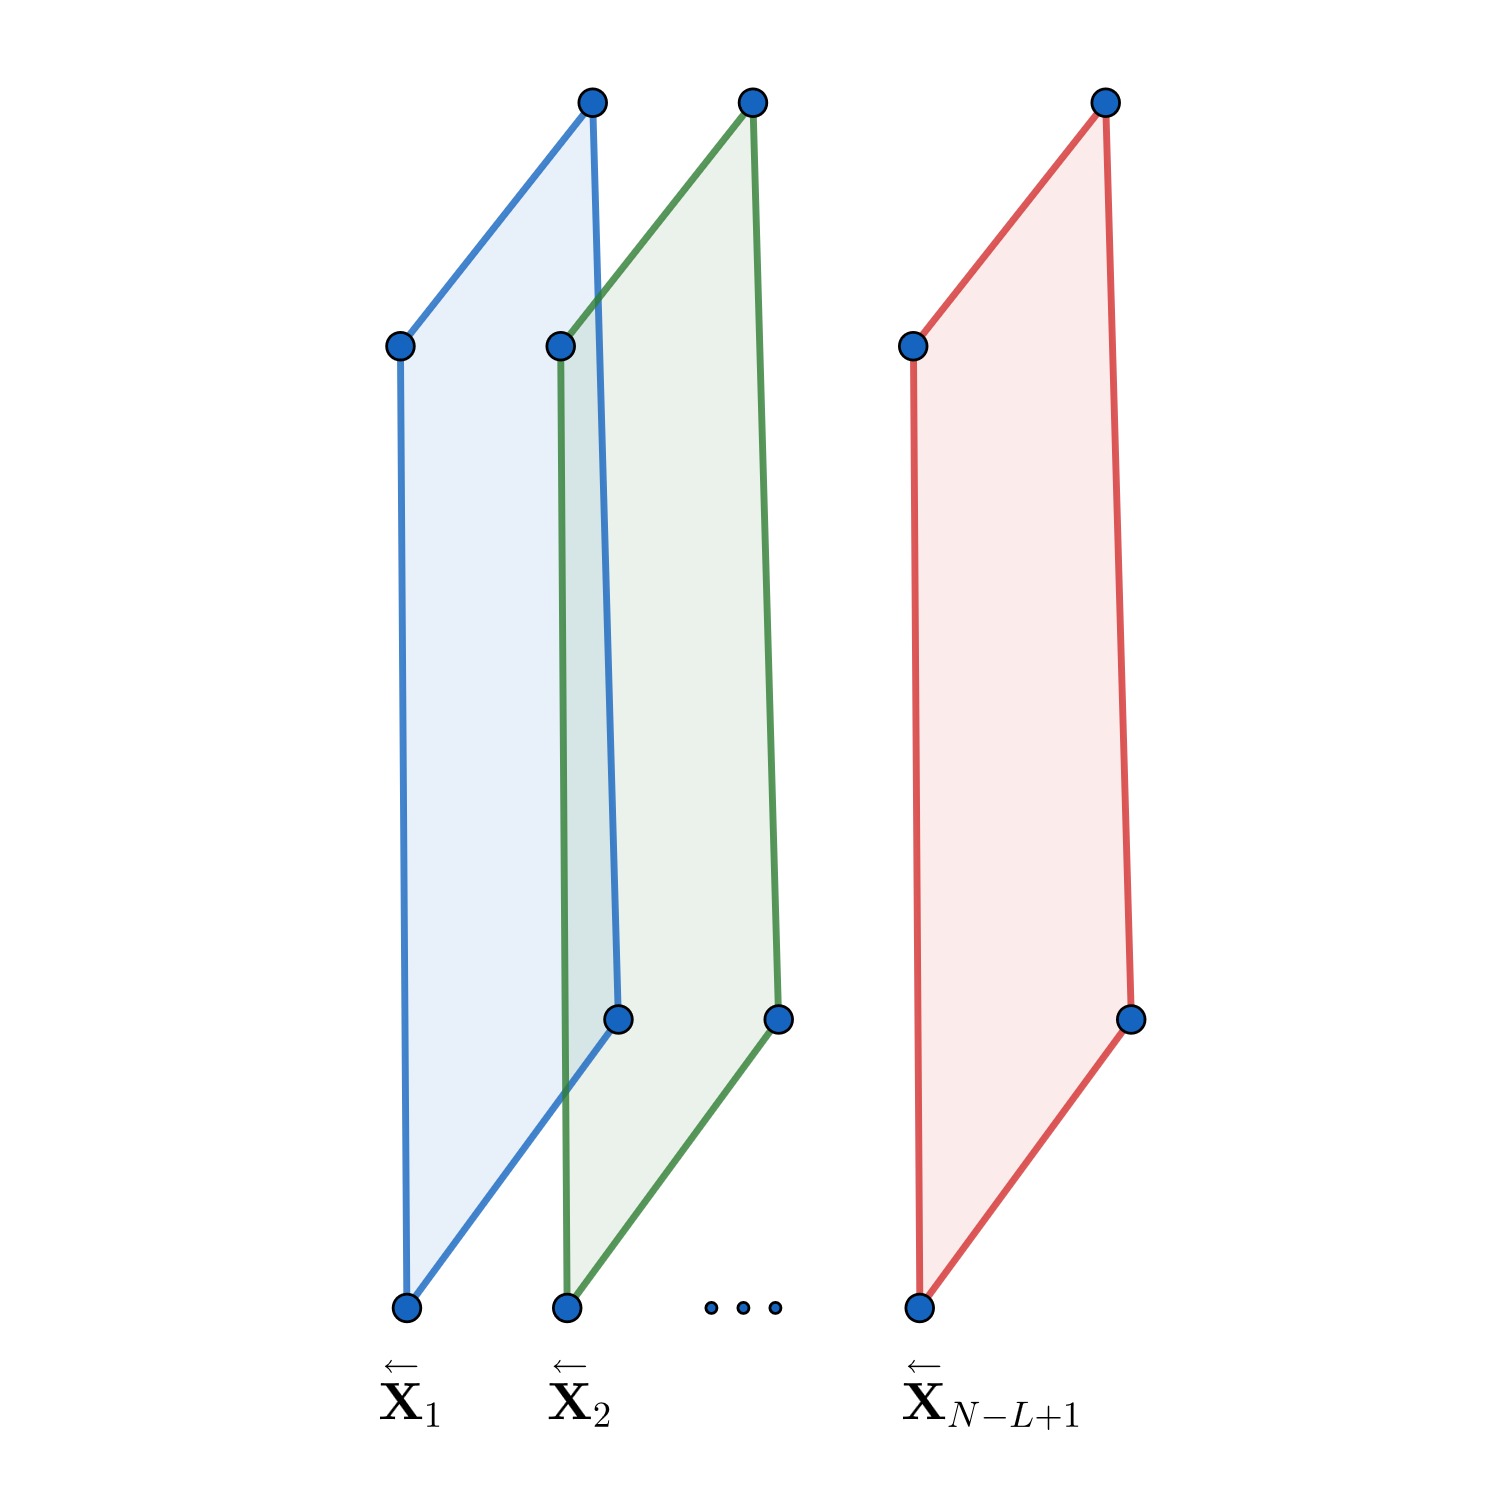
\includegraphics[width=0.4\textwidth, keepaspectratio]{Trajectory_Tensor_2}}
		
		\caption{Two views on trajectory tensor. The left is in terms of signals' trajectory matrices $ \{x_i(t)\}_{i=1}^m $. The right is in terms of delay matrices.}\label{pic:traj_tensor}
	\end{figure}
	
	Similarly to the trajectory matrix we introduce \textit{trajectory tensor} denoted by $ \mathbf{T} $. It is the delay matrices stacked along the second dimension of the tensor, Fig.~\ref{pic:traj_tensor} (left). Equivalent way of constructing the tensor is the following. The $ \mathbf{T} $ is the trajectory matrices $ \mathbf{H}_{x_i} $ stacked along the third dimension, Fig.~\ref{pic:traj_tensor} (right). Therefore the shared phase space of the series is equal to a linear span of all $ \mathbf{H}_{x_i} $. As discussed in the Sec. \ref{sec:one_series}, each trajectory matrix also defines the phase space for the corresponding time series $ x_i(t) $. Finally, we give a 
	
	\begin{Def}		
		The multivariate time series are said to be \emph{interdependent} if they share the common phase space with the same basis.
	\end{Def}
	
	Now assuming observed series interdependence it follows that each $ \mathbf{H}_{x_i} $ has a matrix factorization with the same set of factors. Since the trajectory matrices constructs the trajectory tensor, it has a low-dimensional representation. Using these two corollaries we apply the CP-decomposition to the $ \mathbf{T} $ and obtain $ \mathbf{T} = \sum\limits_{i = 1}^{r} \mathbf{a}_i \otimes \mathbf{b}_i \otimes \mathbf{c}_i $. The CPD is defined by the tensor rank $ r $ and a set of vectors. The vectors are usually composed in full-rank matrices $ A = [\mathbf{a}_1 \ldots \mathbf{a}_r], B = [\mathbf{b}_1 \ldots \mathbf{b}_r], C = [\mathbf{c}_1 \ldots \mathbf{c}_r] $. Denote by $ \boldsymbol{\sigma}_{x_k} $ the $ k $-th row of the $ C $. Finally, with respect to the third-dimension slices of the $ \mathbf{T} $, CPD goes as
	
	\begin{equation}\label{eq:tSSA_decomp}
		\begin{cases}
			\mathbf{H}_{x_1} = \sum\limits_{i = 1}^{r} \boldsymbol{\sigma}_{x_1}(i) \cdot \mathbf{a}_i  \mathbf{b}_i^{\mathsf{T}},  \\
			\mathbf{H}_{x_2} = \sum\limits_{i = 1}^{r} \boldsymbol{\sigma}_{x_2}(i) \cdot \mathbf{a}_i  \mathbf{b}_i^{\mathsf{T}}, \\
			\ldots \\
			\mathbf{H}_{x_m} = \sum\limits_{i = 1}^{r} \boldsymbol{\sigma}_{x_m}(i) \cdot \mathbf{a}_i  \mathbf{b}_i^{\mathsf{T}} .
		\end{cases}
	\end{equation}
	
	The CPD exists for any tensor. In case of the trajectory tensor three properties must hold.
	
	\begin{Th}
		Suppose that the given multivariate time series are interdependent. Then
		
		\begin{enumerate}
			\item Any $ \boldsymbol{\sigma}_{x_k} $ is a non-zero vector
			\item The tensor rank $ r \le L $
			\item Transposition of the trajectory matrix is a a trajectory matrix. The shared phase space for the transposed matrices is the $ \text{Lin}(\{\mathbf{b}_i\}) $
		\end{enumerate}
	\end{Th}
	
	\begin{proof}
		\begin{enumerate}
			\item Suppose some vector has a zero element at the position $ j $ and the other is non-zero in this position. Then two trajectory matrices factorize with a different set of factors. That violates the definition of the series interdependence. Another case is that all $ \boldsymbol{\sigma}_{x_k} $ have a zero element at the position $ j $. Then the matrix $ C $ has a zero row and is not full-ranked. It contradicts to the CPD definition.
			\item As shown in the Sec. \ref{sec:one_series} each time series has its phase space dimension $ \le L $. All delay vectors of every series also lie in the shared phase space $ \text{Lin}(\{\mathbf{a}_i\}) $. Therefore its dimensionality can not become greater.
			\item It is obvious that rows of the trajectory matrices are the delay vectors of size $ N - L + 1 $. Transpose all equalities in the (\ref{eq:tSSA_decomp}). Now it is clear that rows of any $ \mathbf{H}_{x_i} $ belongs to the $ \text{Lin}(\{\mathbf{b}_i\}) $. This is the shared phase space for the new delay vectors.
		\end{enumerate}
	\end{proof}

	\subsection{Time series decomposition}\label{sec:decomposition}
	
	The series are decomposed into additive components using the following conception: \emph{factorization of the trajectory matrix $ \mathbf{H}_{x_k} $ defines the decomposition of the related time series}. This idea comes from the SSA method. Since all $ \mathbf{H}_{x_k} $ have a similar factorization, each time series is decomposed separately.
	
	Trajectory matrices of the series are \emph{hankel} by their definition. That means equal elements along each anti-diagonal of the matrix. It is trivial that any time series of length $ N $ bijectionly corresponds to a hankel matrix of size $ L \times (N - L + 1) $.
	
	Now, we describe the decomposition algorithm. First, the factors of the $ \mathbf{H}_{x_k} $ are arbitrary partitioned into $ s $ groups. The $ s $ is also a chosen number. Then all factors within each partition are summed up. As a result we obtain matrices $ C_1, \ldots, C_s $. If they are all hankel then each $ C $ matrix corresponds to the time series component of the $ x_i(t) $. However, it is almost infeasible even with the trivial series~\cite{ecfb9dc578be43ae9ee8fc88b8ff9151}. Therefore every $ C $ matrix is additionally \emph{hankelized}. This operator averages each matrix's anti-diagonals so the matrix becomes hankel. Denote it as $ \text{Hankel}(\cdot) $. Finally, the algorithm can be written as a chain of identical transformations
	
	\begin{multline}\label{eq:decomp_method_ideal}
		\underline{\mathbf{H}_{x_k}} \overset{1}{=} \sum\limits_{i = 1}^{r} \boldsymbol{\sigma}_{x_k}(i) \cdot \mathbf{a}_i  \mathbf{b}_i^{\mathsf{T}} \overset{2}{=} \sum\limits_{i \in \mathbb{I}_1} \boldsymbol{\sigma}_{x_k}(i) \cdot \mathbf{a}_i  \mathbf{b}_i^{\mathsf{T}} + \ldots + \sum\limits_{i \in \mathbb{I}_s} \boldsymbol{\sigma}_{x_k}(i) \cdot \mathbf{a}_i  \mathbf{b}_i^{\mathsf{T}} \overset{3}{=} \\ \overset{3}{=} C_1 + \ldots + C_s \overset{4}{=} \underline{\text{Hankel}(C_1) + \ldots + \text{Hankel}(C_s)}  \Leftrightarrow x_k(t) = c_1(t) + \ldots c_s(t).
	\end{multline}
	
	Here $ \mathbb{I}_1 \sqcup \ldots \sqcup \mathbb{I}_s = \{1, \ldots, r\} $ are chosen groups of indices. The fourth equality requires proof. But first, consider a hankel operator's property:
	
	\begin{Lem}
		The $ \text{Hankel}(\cdot) $ is a linear operator.
	\end{Lem}
	
	\begin{proof}		
		Having matrices $ A $ and $ B $ with the same size, take their elements from any anti-diagonal. Denote them by $ a_1, \ldots, a_n $ and $ b_1, \ldots, b_n $. Then this anti-diagonal in $ \text{Hankel}(A + B) $ is $ \dfrac{1}{n} \sum\limits^n (a_i + b_i) = \dfrac{1}{n} \sum\limits^n a_i + \dfrac{1}{n} \sum\limits^n b_i $. It exactly results in a sum of $ \text{Hankel}(A) $ and $ \text{Hankel}(B) $ anti-diagonals.
		
		Secondly, having a scalar $ \alpha $ it is trivial that $ \dfrac{1}{n} \sum\limits^n \alpha \cdot a_i = \alpha \dfrac{1}{n} \sum\limits^n a_i $. Hence we derive $ \text{Hankel}(\alpha A) = \alpha \text{Hankel}(A) $.
	\end{proof}
	
	Now recall that the $ \mathbf{H}_{x_k} $ is hankel. Combining it with the previous lemma, apply $ \text{Hankel}(\cdot) $ to the $ \mathbf{H}_{x_k} = C_1 + \ldots + C_s $. This proofs the fourth equality at (\ref{eq:decomp_method_ideal}). Therefore, we have shown the correctness of the decomposition algorithm.
	
	\subsection{Optimal decomposition problem}\label{sec:optimal_decomp}
	
	To eliminate ambiguity in the partitioning of the $ \mathbf{H}_{x_k} $ factors, we restrict $ C_j $ matrices to be hankel. Thus, the fourth step of the decomposition algorithm (\ref{eq:decomp_method_ideal}) becomes unnecessary. In addition, such partitioning completely fulfills the decomposition concept. 
	
	Now we formulate the decomposition problem as a system of matrix equations. Take the first equality from the (\ref{eq:decomp_method_ideal}) and apply the hankel operator to the both sides. Recall that the $ \mathbf{H}_{x_k} $ is hankel. Also take the very same equality as it is. We obtain
	
	\begin{equation*}
		\begin{cases*}
			\mathbf{H}_{x_k} = \sum\limits_{i = 1}^{r} \boldsymbol{\sigma}_{x_k}(i) \cdot \mathbf{a}_i  \mathbf{b}_i^{\mathsf{T}} \\
			\mathbf{H}_{x_k} = \sum\limits_{i = 1}^{r} Hankel(\boldsymbol{\sigma}_{x_k}(i) \cdot \mathbf{a}_i  \mathbf{b}_i^{\mathsf{T}})
		\end{cases*}
	\end{equation*}
	
	Then subtract the second from the first and denote by $ H_i $ a $ \boldsymbol{\sigma}_{x_k}(i) \cdot \mathbf{a}_i  \mathbf{b}_i^{\mathsf{T}} - Hankel(\boldsymbol{\sigma}_{x_k}(i) \cdot \mathbf{a}_i  \mathbf{b}_i^{\mathsf{T}}) $. It is called the \emph{hankel residual matrix} of the $ i $-th factor. Therefore we get
	
	\begin{equation}\label{eq:residuals_equation}
		H_1 + \ldots + H_r = 0 \text{. Or equally } H_r = - \sum\limits_{j = 1}^{r - 1} H_j.
	\end{equation}
	
	Finally, the condition on the $ C_i $ to be hankel is reformulated as the residual matrices sum up to zero within each partition group. The system of matrix equations is the following
	
	\begin{equation*}
		\sum_{k \in \mathbb{I}_i} H_k = 0 \  \forall i \in 1, \ldots, s.
	\end{equation*}
	
	Without loss of generality, we set $ s $ equals two. If this problem is solved then the resulting groups of the factors can be further partitioned. Hence any number of the time series components can be obtained. Moreover, for any $ \mathbf{H}_{x_k} $ its residual matrices are linearly dependent as follows from the (\ref{eq:residuals_equation}). Thus, the partition group for the $ H_r $ is uniquely defined if all other residuals are already partitioned. This matrix can be discarded. We also assume all $ H_j $ to be non-zero matrices. Otherwise, the zero residual matrix alone and all the rest make the desired partition on two groups. This assumption implies each of the groups to have at least two residual matrices. Finally, for any $ H_j $ matrix introduce an indicator-variable $ \beta_j \in \{0, 1\} $. It shows what group the residual matrix belongs to. Denote by $ \boldsymbol{\beta} $ a vector $ (\beta_1 \ldots \beta_{r-1})^{\text{T}} $. The decomposition problem is to find $ \boldsymbol{\beta} $ such that
	
	\begin{equation}\label{eq:first_optimal_decomp}
		\begin{cases*}
			\sum\limits_{j = 1}^{r - 1} \beta_j H_j = 0, \\
			\beta_j \in \{0, 1\} \ \forall j \in 1 \ldots r, \\
			\sum\limits_{i = 1}^{r - 1} \beta_j \ge 2.
		\end{cases*}
	\end{equation}
	
	The \cite{ecfb9dc578be43ae9ee8fc88b8ff9151} shows that even for trivial time series such a problem is infeasible. Now we transform it into a feasible one. First, vectorize each $ H_i $ and stack resulting vectors into the matrix denoted by $ \Lambda $. Then the first equation in the (\ref{eq:first_optimal_decomp}) is equivalent to the $ \Lambda \boldsymbol{\beta} = 0 $. Second, change the problem of solving the system of equations to an optimization problem. Let's find such $ \boldsymbol{\beta} $ that delivers minimum to the norm of the $ \Lambda \boldsymbol{\beta} $. The changed problem is
	
	\begin{equation}\label{eq:decomp_search_final}
		\begin{cases*}
			\lVert \Lambda \boldsymbol{\beta} \rVert \to \underset{\boldsymbol{\beta}}{\min}, \\
			\beta_j \in \{0, 1\} \ \forall j \in 1 \ldots r, \\
			\sum\limits_{i = 1}^{r - 1} \beta_j \ge 2.
		\end{cases*}
	\end{equation}
	
	Call solution of the (\ref{eq:decomp_search_final}) the \emph{optimal series decomposition}. The problem itself is an Integer Least Squares (ILS) problem, which is proved to be NP-hard~\cite{van1981another}. The final result of the section is
	
	\begin{Th}
		The optimal series decomposition is an NP-hard problem.
	\end{Th}
	
	In spite of the complexity, methods and heuristics exist to reduce the ILS to computationally effective problems~\cite{Grafarend2022}.
	
	\subsection{Time series forecasting}\label{sec:tssa_forecast}
	
	Using the build shared phase space each time series is forecast individually. We make a one-step forecast to estimate $ x(N + 1) $. Phase trajectory of the series is a sequence of the delay vectors $ \{ \delayV{t} \} $. The whole trajectory belongs to the phase space $ \text{Lin}(\{\mathbf{a}_i\}) $. Continuation of the trajectory is the $ \delayV{N + 1} $. Therefore $ \delayV{N + 1} \in \text{Lin}(\{\mathbf{a}_i\}) $. At the same time $ x(N + 1) $ is the last component of the $ \delayV{N + 1} $. Now, recall the $ A $ matrix introduced in the Sec. \ref{sec:tssa_method}. The system of linear equation to find $ x(N + 1) $ is
	
	\begin{align}\label{eq:main_pred_for_A}
		\delayV{N + 1} = A \boldsymbol{\lambda} \text{ or equally } &\begin{cases}
			\mathbf{x}_{kn} = A_{kn} \boldsymbol{\lambda}  \\
			x(N + 1) = \mathbf{a}_{pr}^{\mathsf{T}} \boldsymbol{\lambda}
		\end{cases}, \text{ where } \\
		A &= \left( \dfrac{A_{kn}}{\mathbf{a}_{pr}^{\mathsf{T}}} \right), \nonumber \\
		\delayV{N + 1} &= (\mathbf{x}_{kn} \  x(N + 1))^{\mathsf{T}}. \nonumber
	\end{align}
	
	The delay vector and the matrix are broken into two blocks associated with the \emph{known} and \emph{predicted} part of the series. The forecast is made using the second equation in the (\ref{eq:main_pred_for_A}). Therefore vector $ \boldsymbol{\lambda} \in \mathbb{R}^r $ is to be found from the first equation in the (\ref{eq:main_pred_for_A}). It is a system of linear equations with the matrix $ A_{kn} $. The matrix has a rank at least $ r - 1 $ since $ A $ matrix is full-ranked. However we assume $ A_{kn} $ to have rank $ r $ too. As experiments show this is not burdensome. In addition, the linear system is overdetermined since $ r \le L $ (see Sec. \ref{sec:tssa_method}). Therefore its solution is given by the least-squares formula $ \boldsymbol{\lambda} = (A_{kn}^T A_{kn})^{-1} A_{kn}^T \mathbf{x}_{kn} $. After replacing it in (\ref{eq:main_pred_for_A}) we obtain the forecast formula
	
	\begin{equation}\label{eq:tssa_pred}
		\hat{x}(N + 1) = \mathbf{a}_{pr}^{\mathsf{T}} (A_{kn}^T A_{kn})^{-1} A_{kn}^T \mathbf{x}_{kn}.
	\end{equation}
	
	Denote by the $ \mathbf{d} $ a vector $ \mathbf{a}_{pr}^{\mathsf{T}} (A_{kn}^T A_{kn})^{-1} A_{kn}^T $. Once computed, it can be reused to make the forecast for any steps further. Now rewrite the (\ref{eq:tssa_pred}) in terms of the $ x(t) $:
	
	\begin{equation*}\label{eq:autoregr}
		x(t) = \sum\limits_{i = 1}^{L - 1} d_i \cdot x(t - i)
	\end{equation*}
	
	This expression reveals the property of the forecast sequence $ \{\hat{x}(N + i)\}_{i=1}^{\infty} $.
	
	\begin{Th}		
		The model of the tSSA's forecast is \emph{autoregressive} $ AR(L - 1) $. The coefficients $ d_i $ found in the (\ref{eq:tssa_pred}) completely define behavior of the forecast sequence.
	\end{Th}
	
	\section{Computational experiment}	
	
	In the current section we obtain the decomposition and the forecast of multivariate time series. We also compare the tSSA with the other methods: the mSSA, the VAR, and the RNN. The latter two are only for the forecast. Moreover,to measure quality of the decomposition we introduce special metrics. They are motivated by the corresponding analysis in the Sec. \ref{sec:decomposition}.
	
	\begin{Def}
		The \emph{absolute hankel error} of the matrix M is 
		
		\[
		\text{AHE} = \lVert M - \text{Hankel}(M) \rVert_F
		\] 
		
	\end{Def}	
	
	\begin{Def}		
		
		The \emph{relative hankel error} of the matrix M is 
		
		\[
		\text{RHE} = \frac{\text{AHE}}{\lVert M \rVert_F} 
		\] 		
		
	\end{Def}
	
	The AHE is proportional to the total variance of the matrix's anti-diagonals. The RHE is AHE's more interpretable modification. In the Sec. \ref{sec:decomposition} matrices $ C_i $ were introduced. They correspond to the time series components. In the Sec. \ref{sec:optimal_decomp} the optimal decomposition was introduced. It is basically minimizing of the AHE for the $ C_i $ matrices. Hence, the AHE and the RHE are computed for the $ C_i $ in the further experiments. Denote by $ \overline{\text{RHE}}_{\text{ts}} $ the mean RHE across all $ C_i $ of the time series \textit{ts}. Denote by $ \overline{\text{RHE}} $ the mean $ \overline{\text{RHE}}_{\text{ts}} $ across all given time series.
	
	To measure forecast quality for the time series \textit{ts} we use standard metrics: the \emph{mean squared error} $ \text{MSE}_{\text{ts}} $ and the \emph{mean absolute percentage error} $ \text{MAPE}_{\text{ts}} $. Denote by $ \overline{\text{MSE}} $ and $ \overline{\text{MAPE}} $ their mean across all given time series.
	
	Two sets of data are involved in the experiment. First, electricity consumption and electricity price time series (Fig. \ref{fig:electr_data}). Second, inertial unit measurements; three time series are from an accelerometer and three from a gyroscope~\cite{accelerometryData} (Fig. \ref{fig:motion_data}). Walking movements are detected here. We assume the series' interdependence (see Sec. \ref{sec:tssa_method}) based on the economical/physical premises. The series have a length of $ \approx 3 \cdot 10^3 $. About $ 20\% $ of them are deferred test samples for the forecast quality evaluation.
	
	\begin{figure}[h]
		\centering
		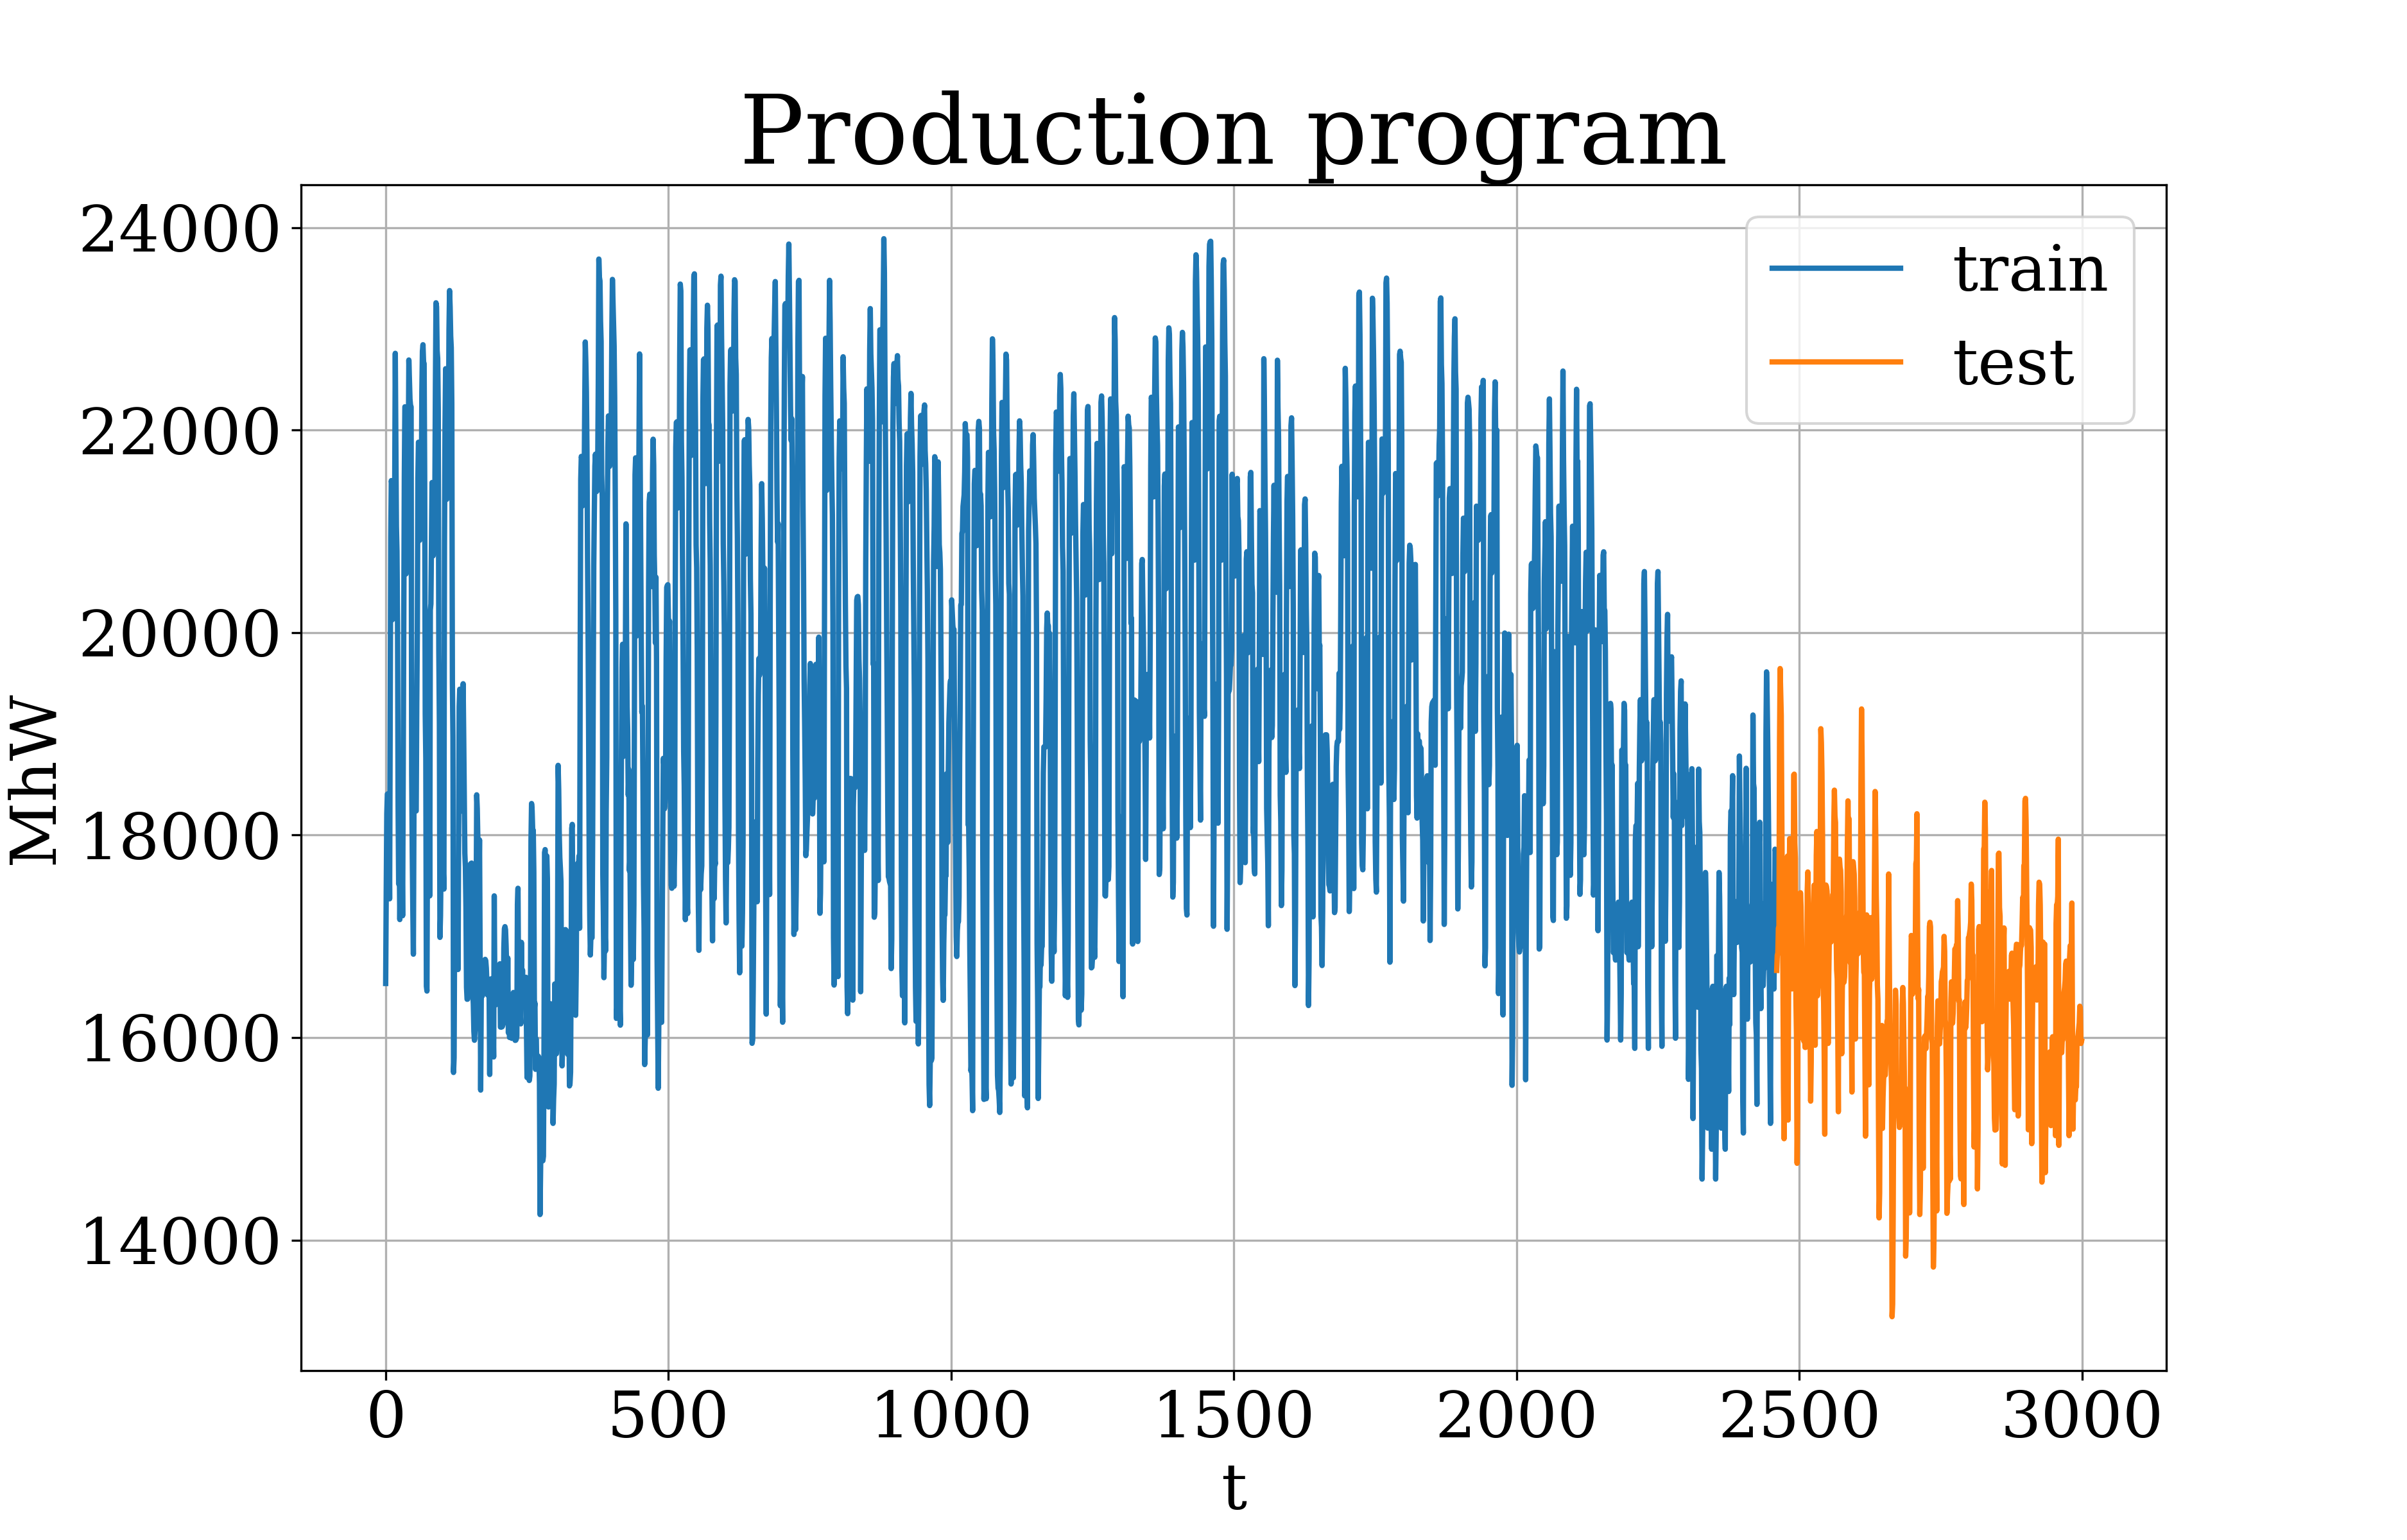
\includegraphics[width=0.48\textwidth, keepaspectratio]{Electricity_Production}
		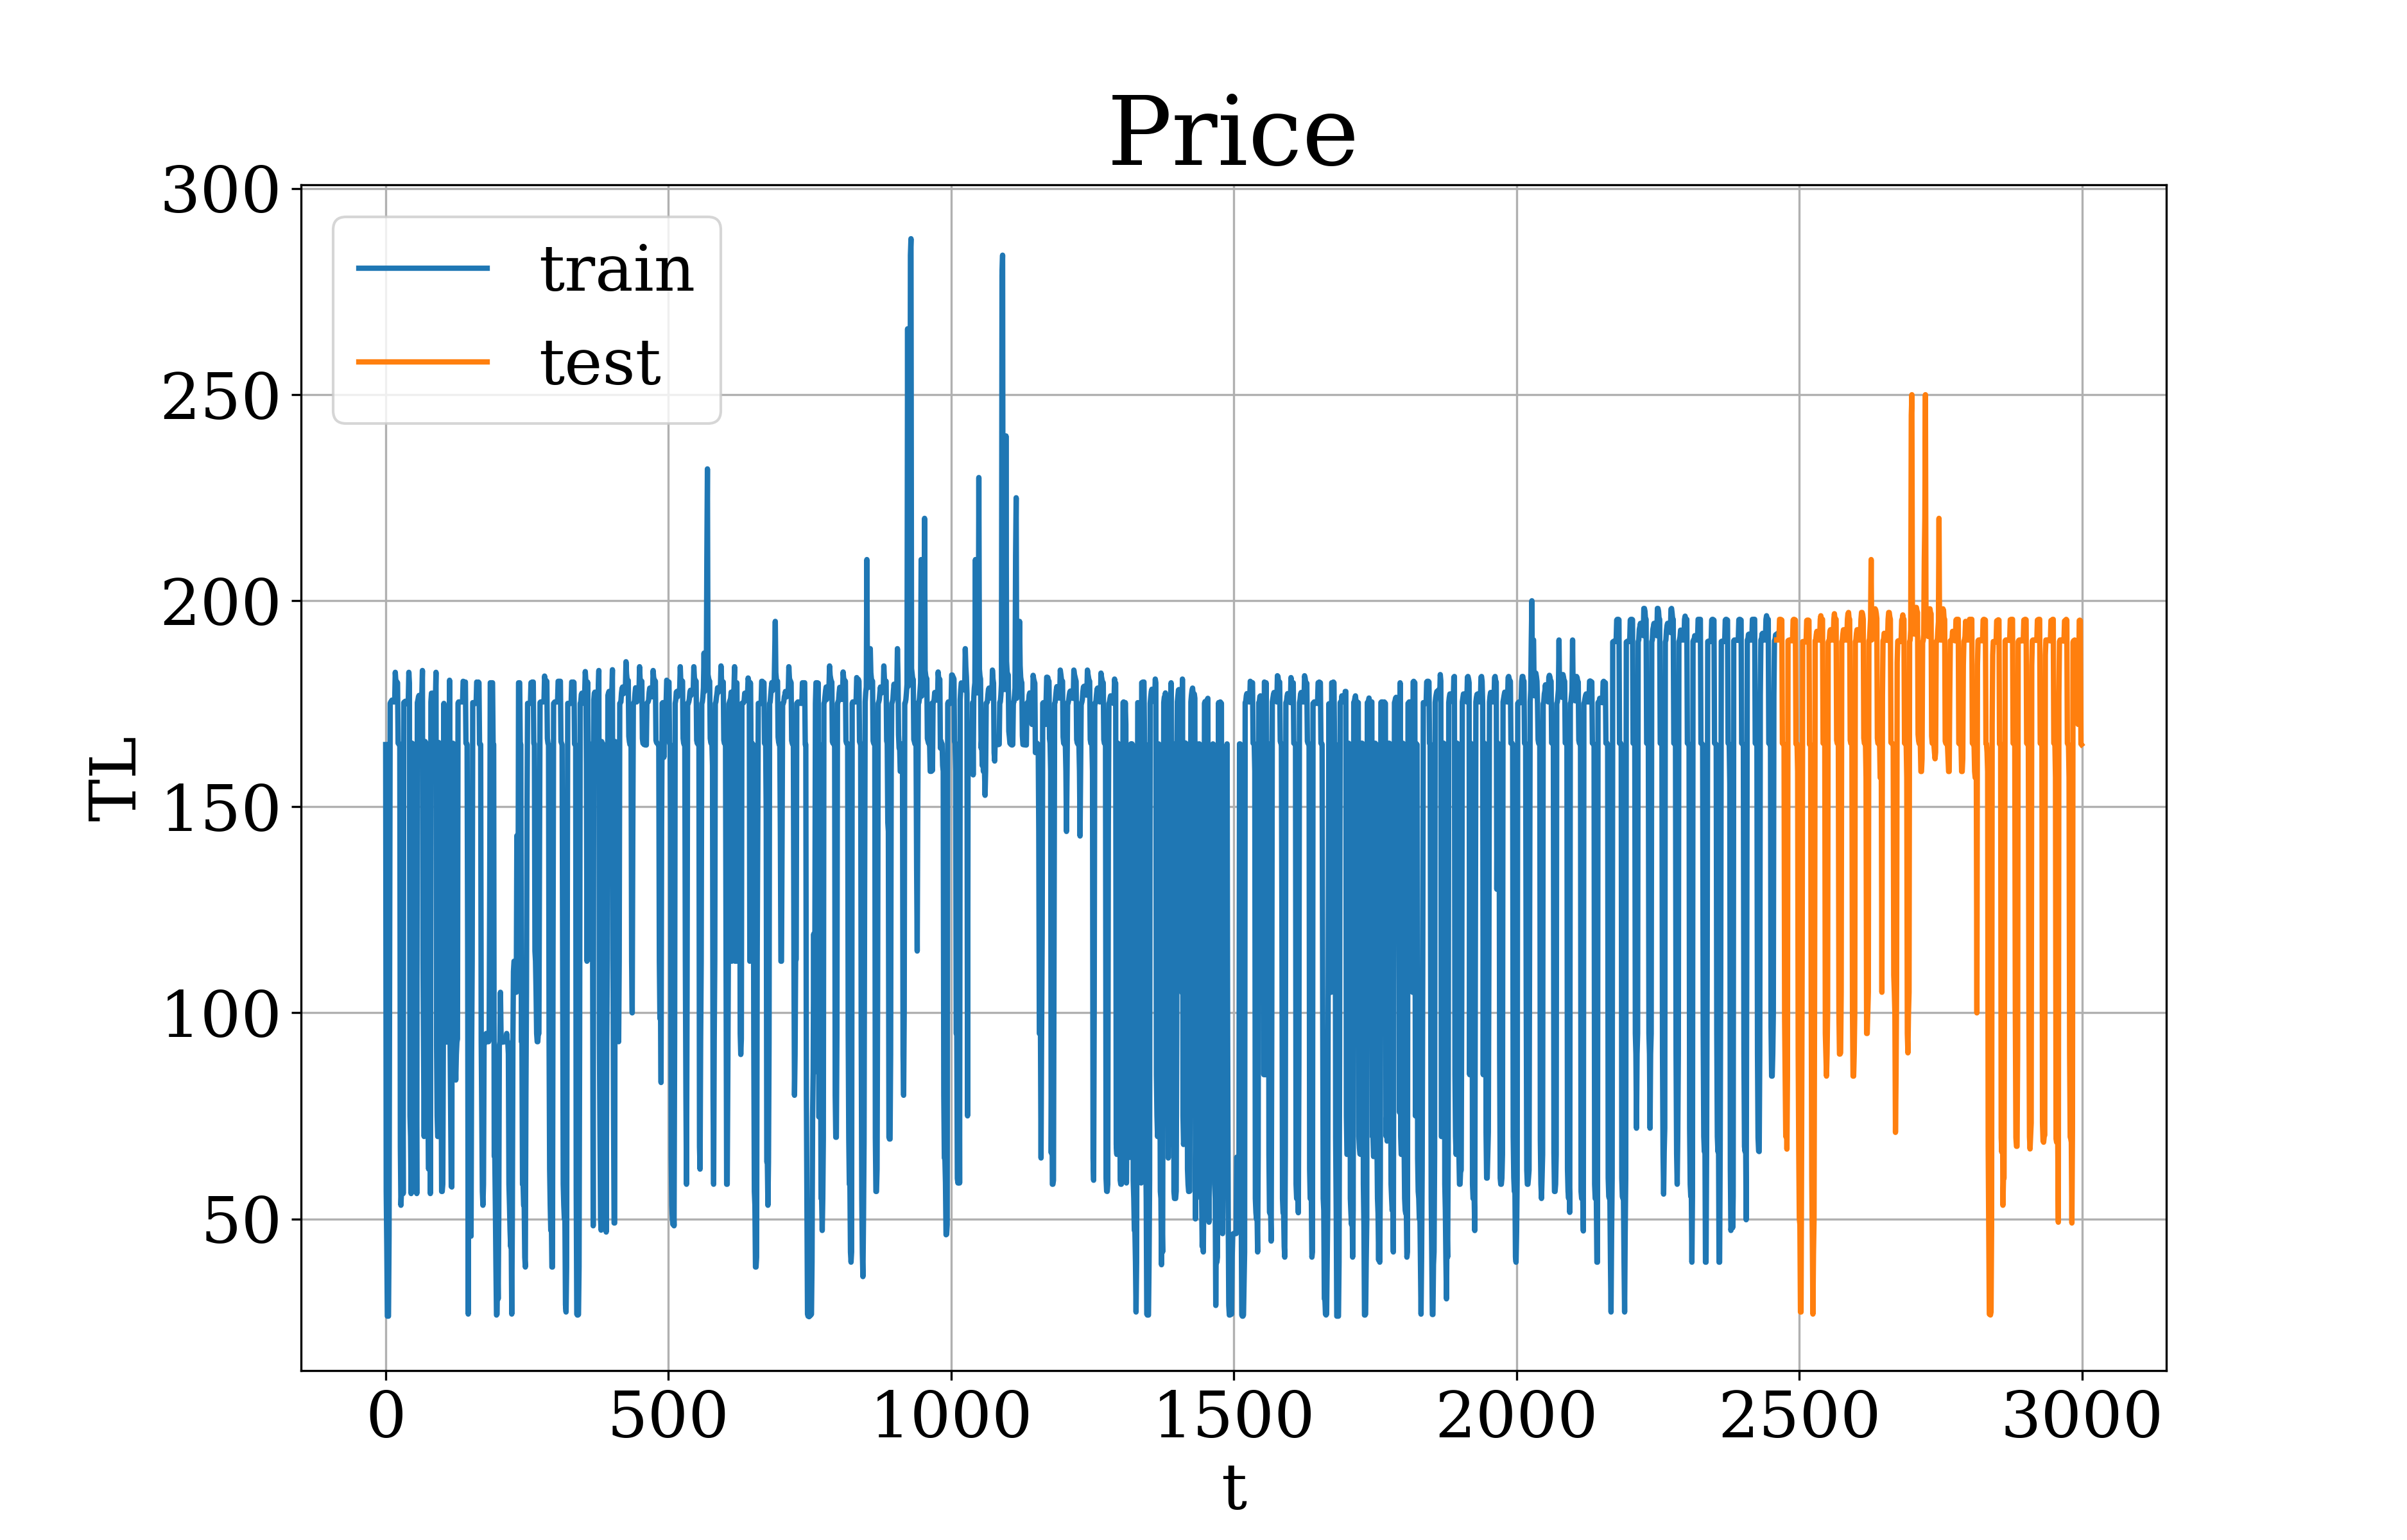
\includegraphics[width=0.48\textwidth, keepaspectratio]{Electricity_Price}
		\caption{Time series for electricity consumption and its price}\label{fig:electr_data}
	\end{figure}
	
	\begin{figure}[h]
		\centering
		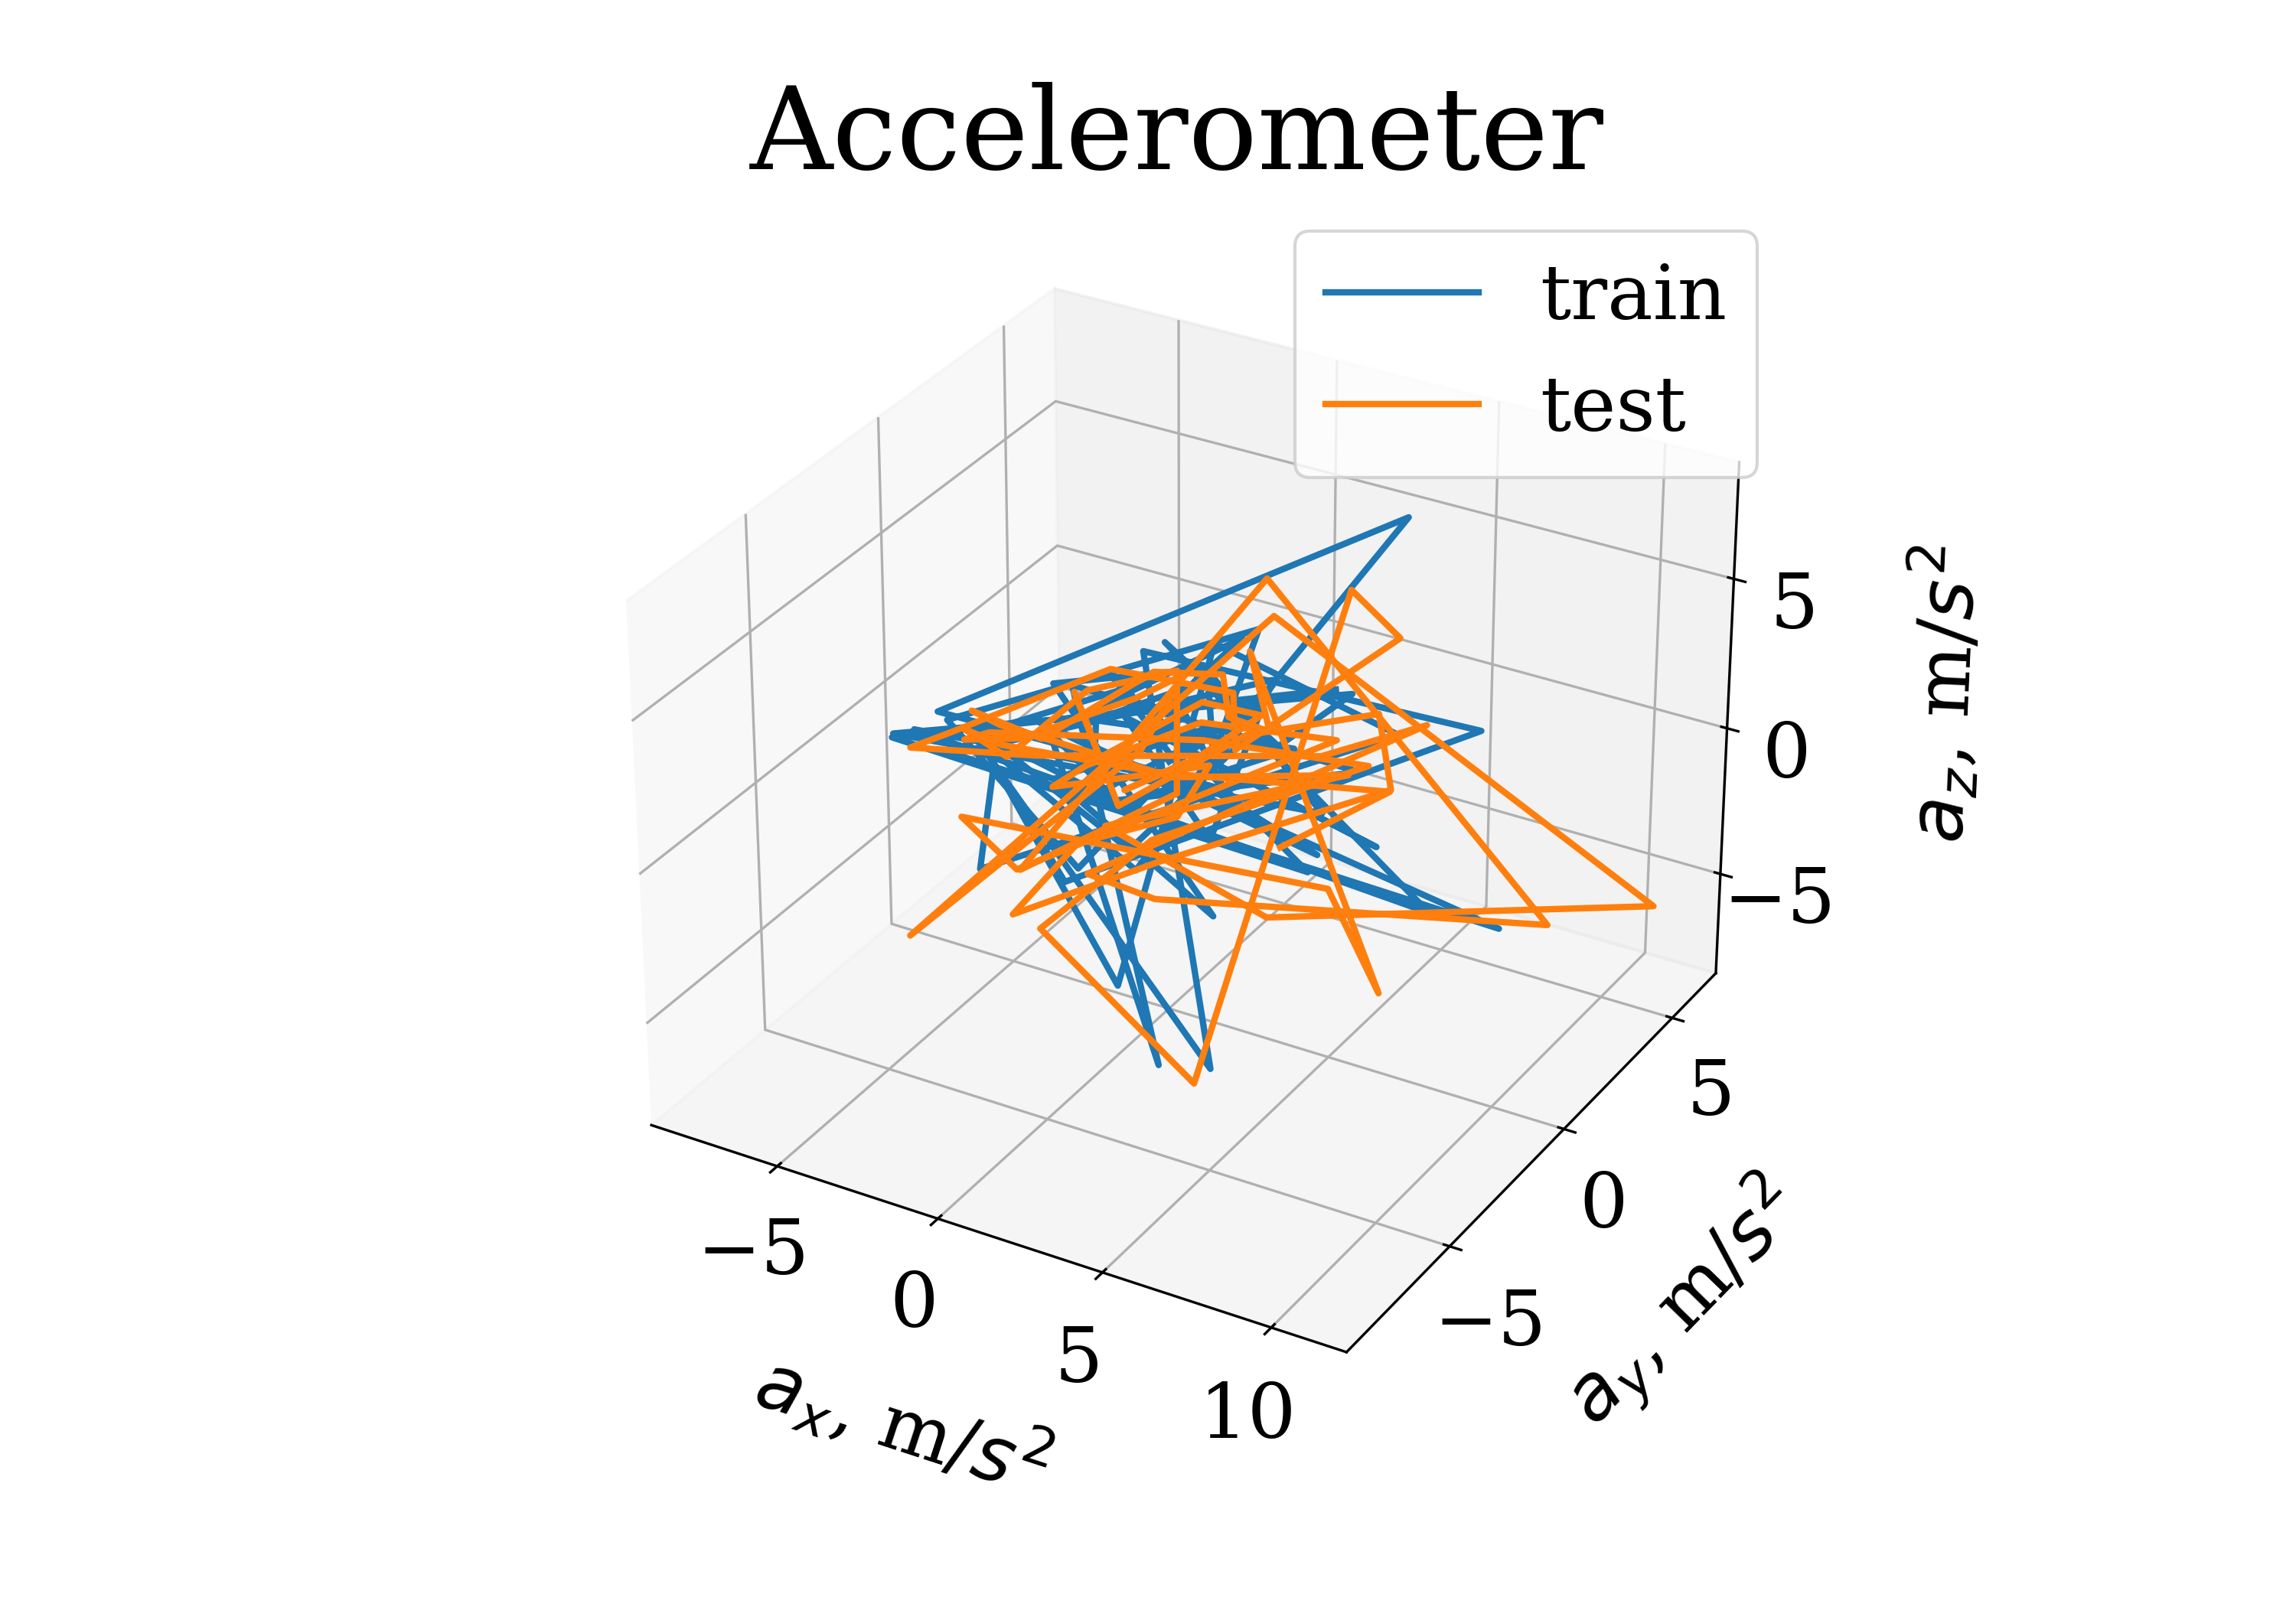
\includegraphics[width=0.48\textwidth, keepaspectratio]{acceleromter_example.png}
		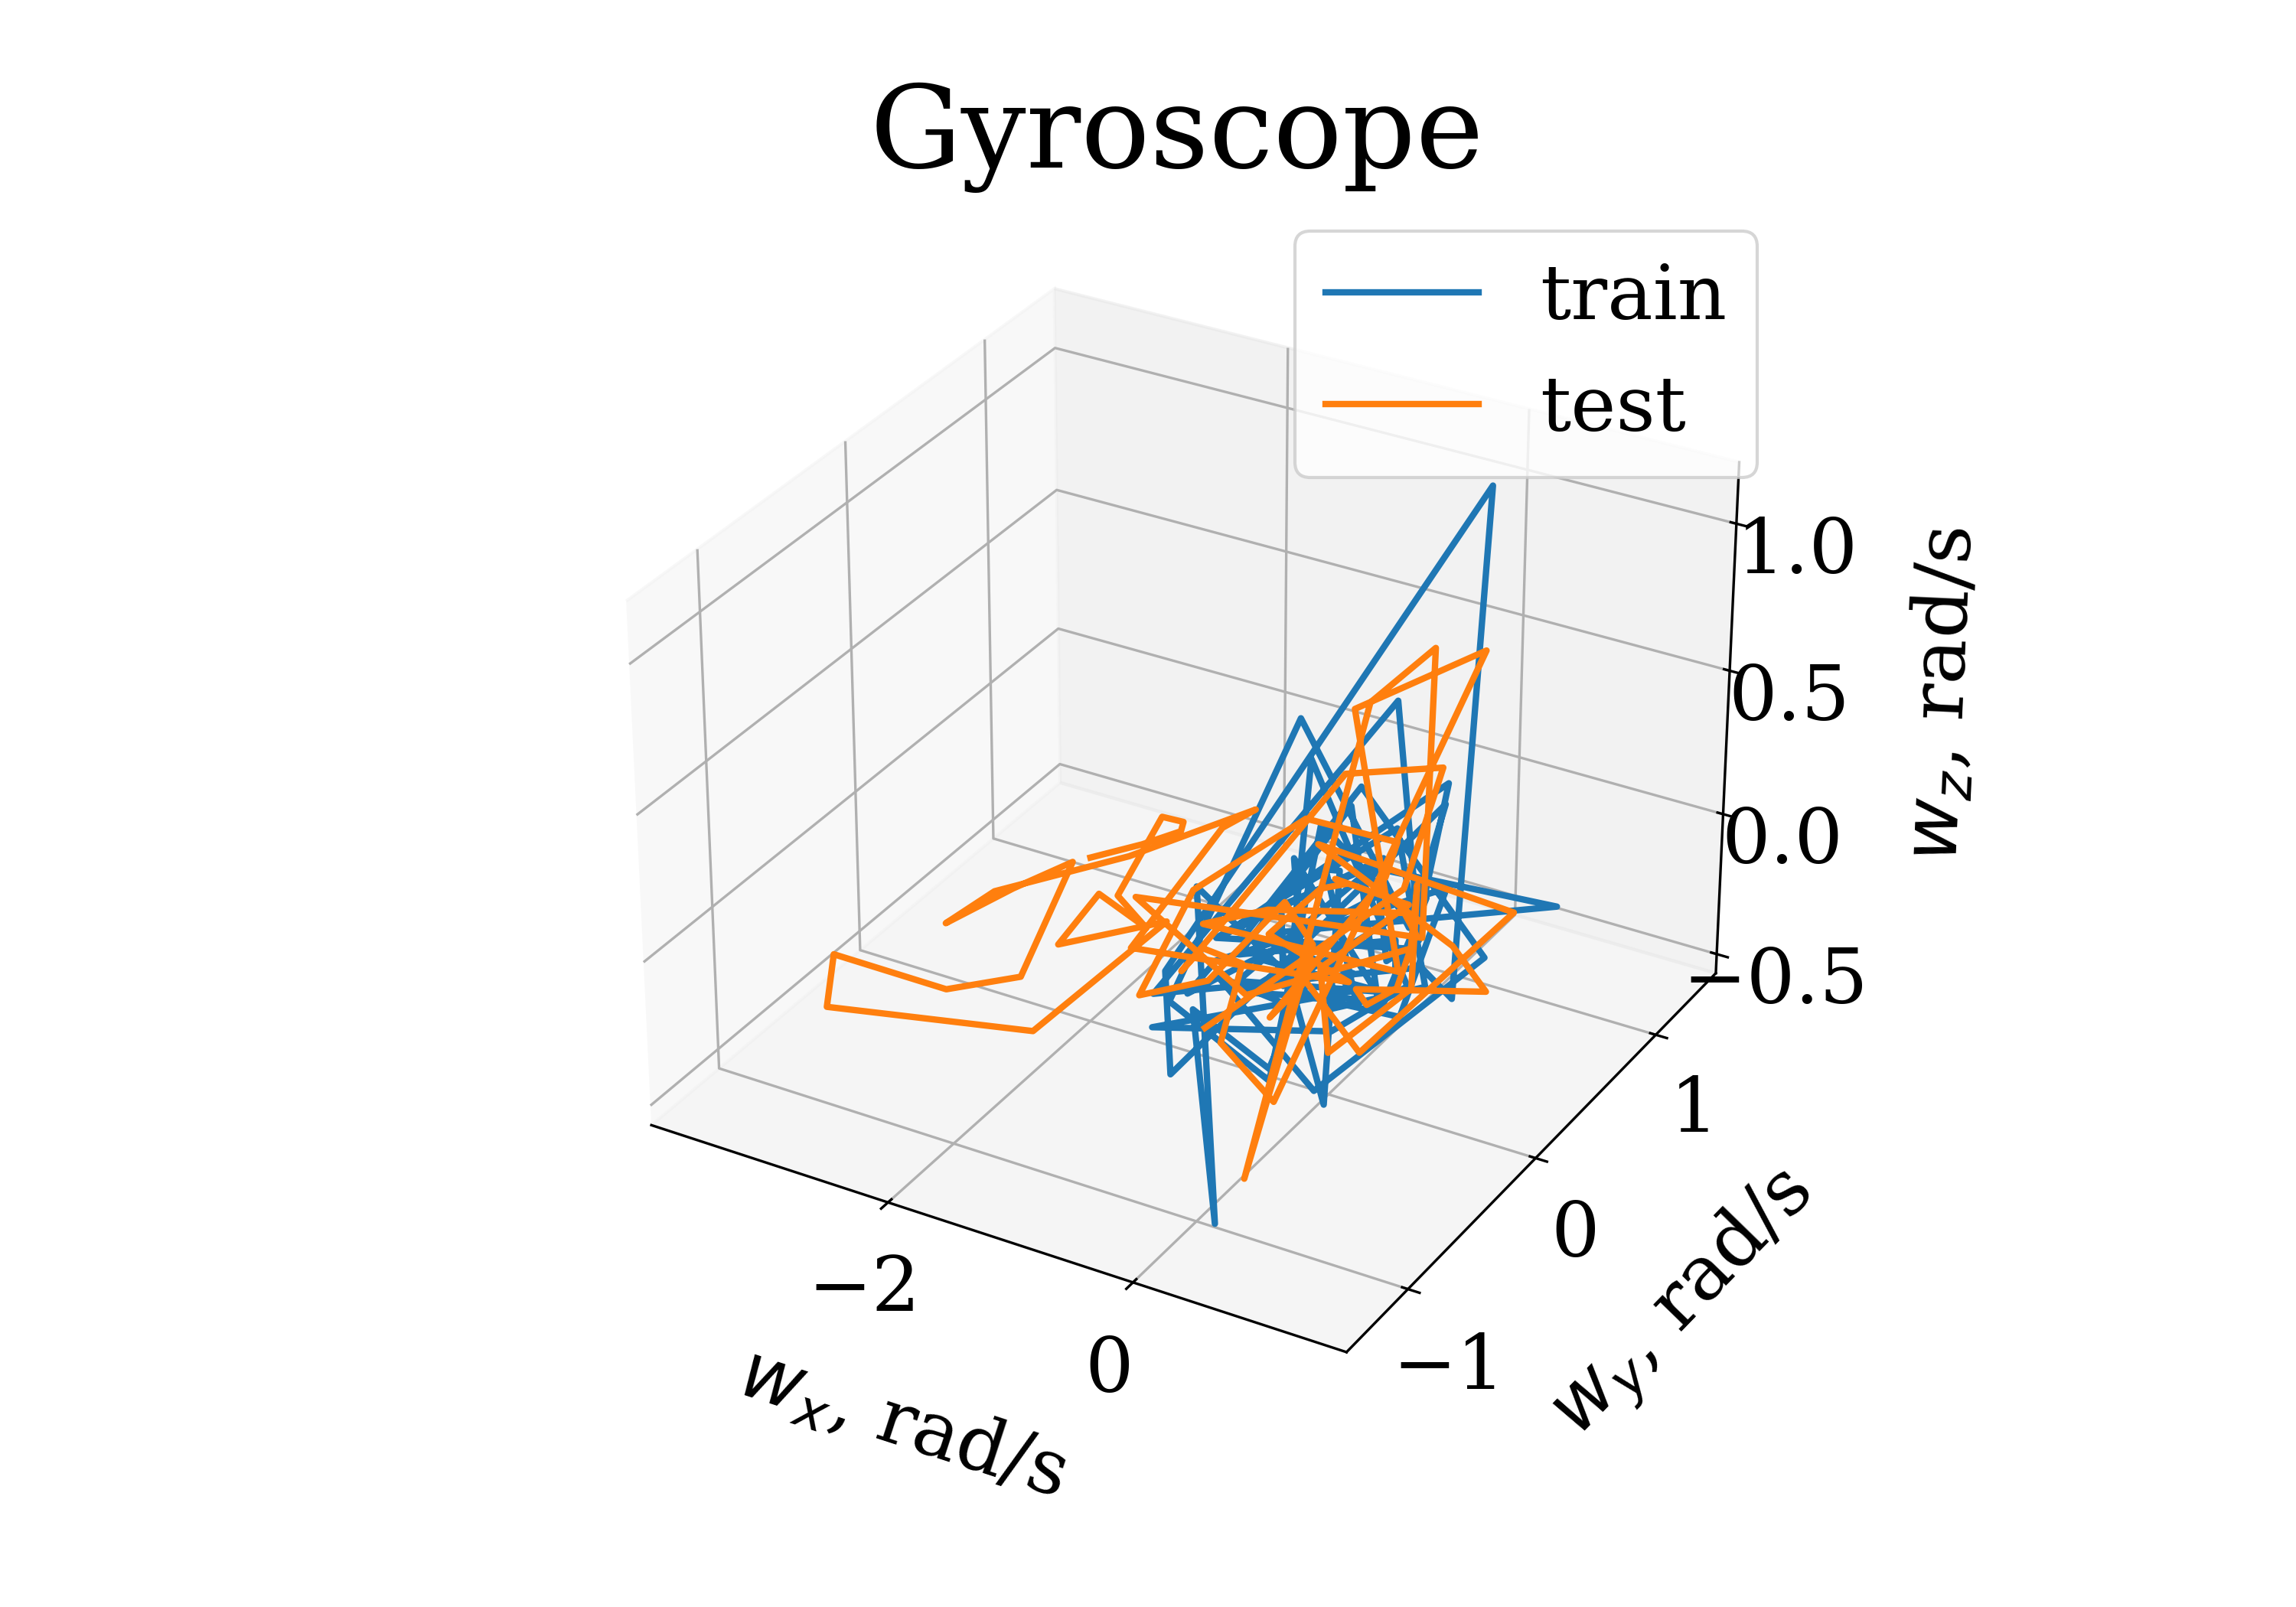
\includegraphics[width=0.48\textwidth, keepaspectratio]{gyro_example.png}
		\caption{Time series for linear and angular accelerations}\label{fig:motion_data}
	\end{figure}
	
	Now we describe some computational features of the tSSA application. First, tensor rank computation is NP-hard~\cite{HASTAD1990644}. Its specific number is explicitly indicated whenever needed. Second, an algorithm for CPD computation is the ALS~\cite{kolda_tensors}. Since it has an approximation error, the (\ref{eq:tSSA_decomp}) is not precise on practice. Therefore, computed forecast and decomposition are not precise too. The approximation errors are specified whenever needed. Third, the ILS problem (\ref{eq:decomp_search_final}) must be solved to find the series decomposition. But the involved matrix $ \Lambda $ has a large row dimension. To shorten computation, only several hundred rows are left. However, it is still much greater then the size of the sought $ \boldsymbol{\beta} $ vector.	Finally the $ L $ value (see Sec. \ref{sec:one_series}) is $ 500 $ for the electricity data and $ 1000 $ for the inertial unit data. This parameter also has a meaning for the other models. For the RNN it is the length of the initial series input to further make the forecast. For the VAR it is a maximal lag number~\cite{3b1355aedd1041f1853e609a410576f3}. 
	
	\subsection{Data availability}
	
	Electricity consumption dataset is available at \url{https://sourceforge.net/p/mvr/code/HEAD/tree/data/TurkElectricityConsumption.csv}. Accelerometry data is available at \url{https://data.mendeley.com/datasets/45f952y38r/5}.
	
	\subsection{Results and discussion}
	
	We begin with the tSSA's forecast results. First, relationship between the forecast metrics and the trajectory tensor's rank is depicted in the Fig. \ref{fig:mse_mape_electr} and \ref{fig:mse_mape_motion}. We see that the forecast quality decreases with the greater ranks for both metrics. Furthermore, \emph{overtraining effect} is present as the MAPE metric increases after reaching a minimum. Nonetheless, the CPD's approximation error decreases monotonously, see Fig. \ref{fig:cpd_errors}.
	
	\begin{figure}[h]
		\centering
		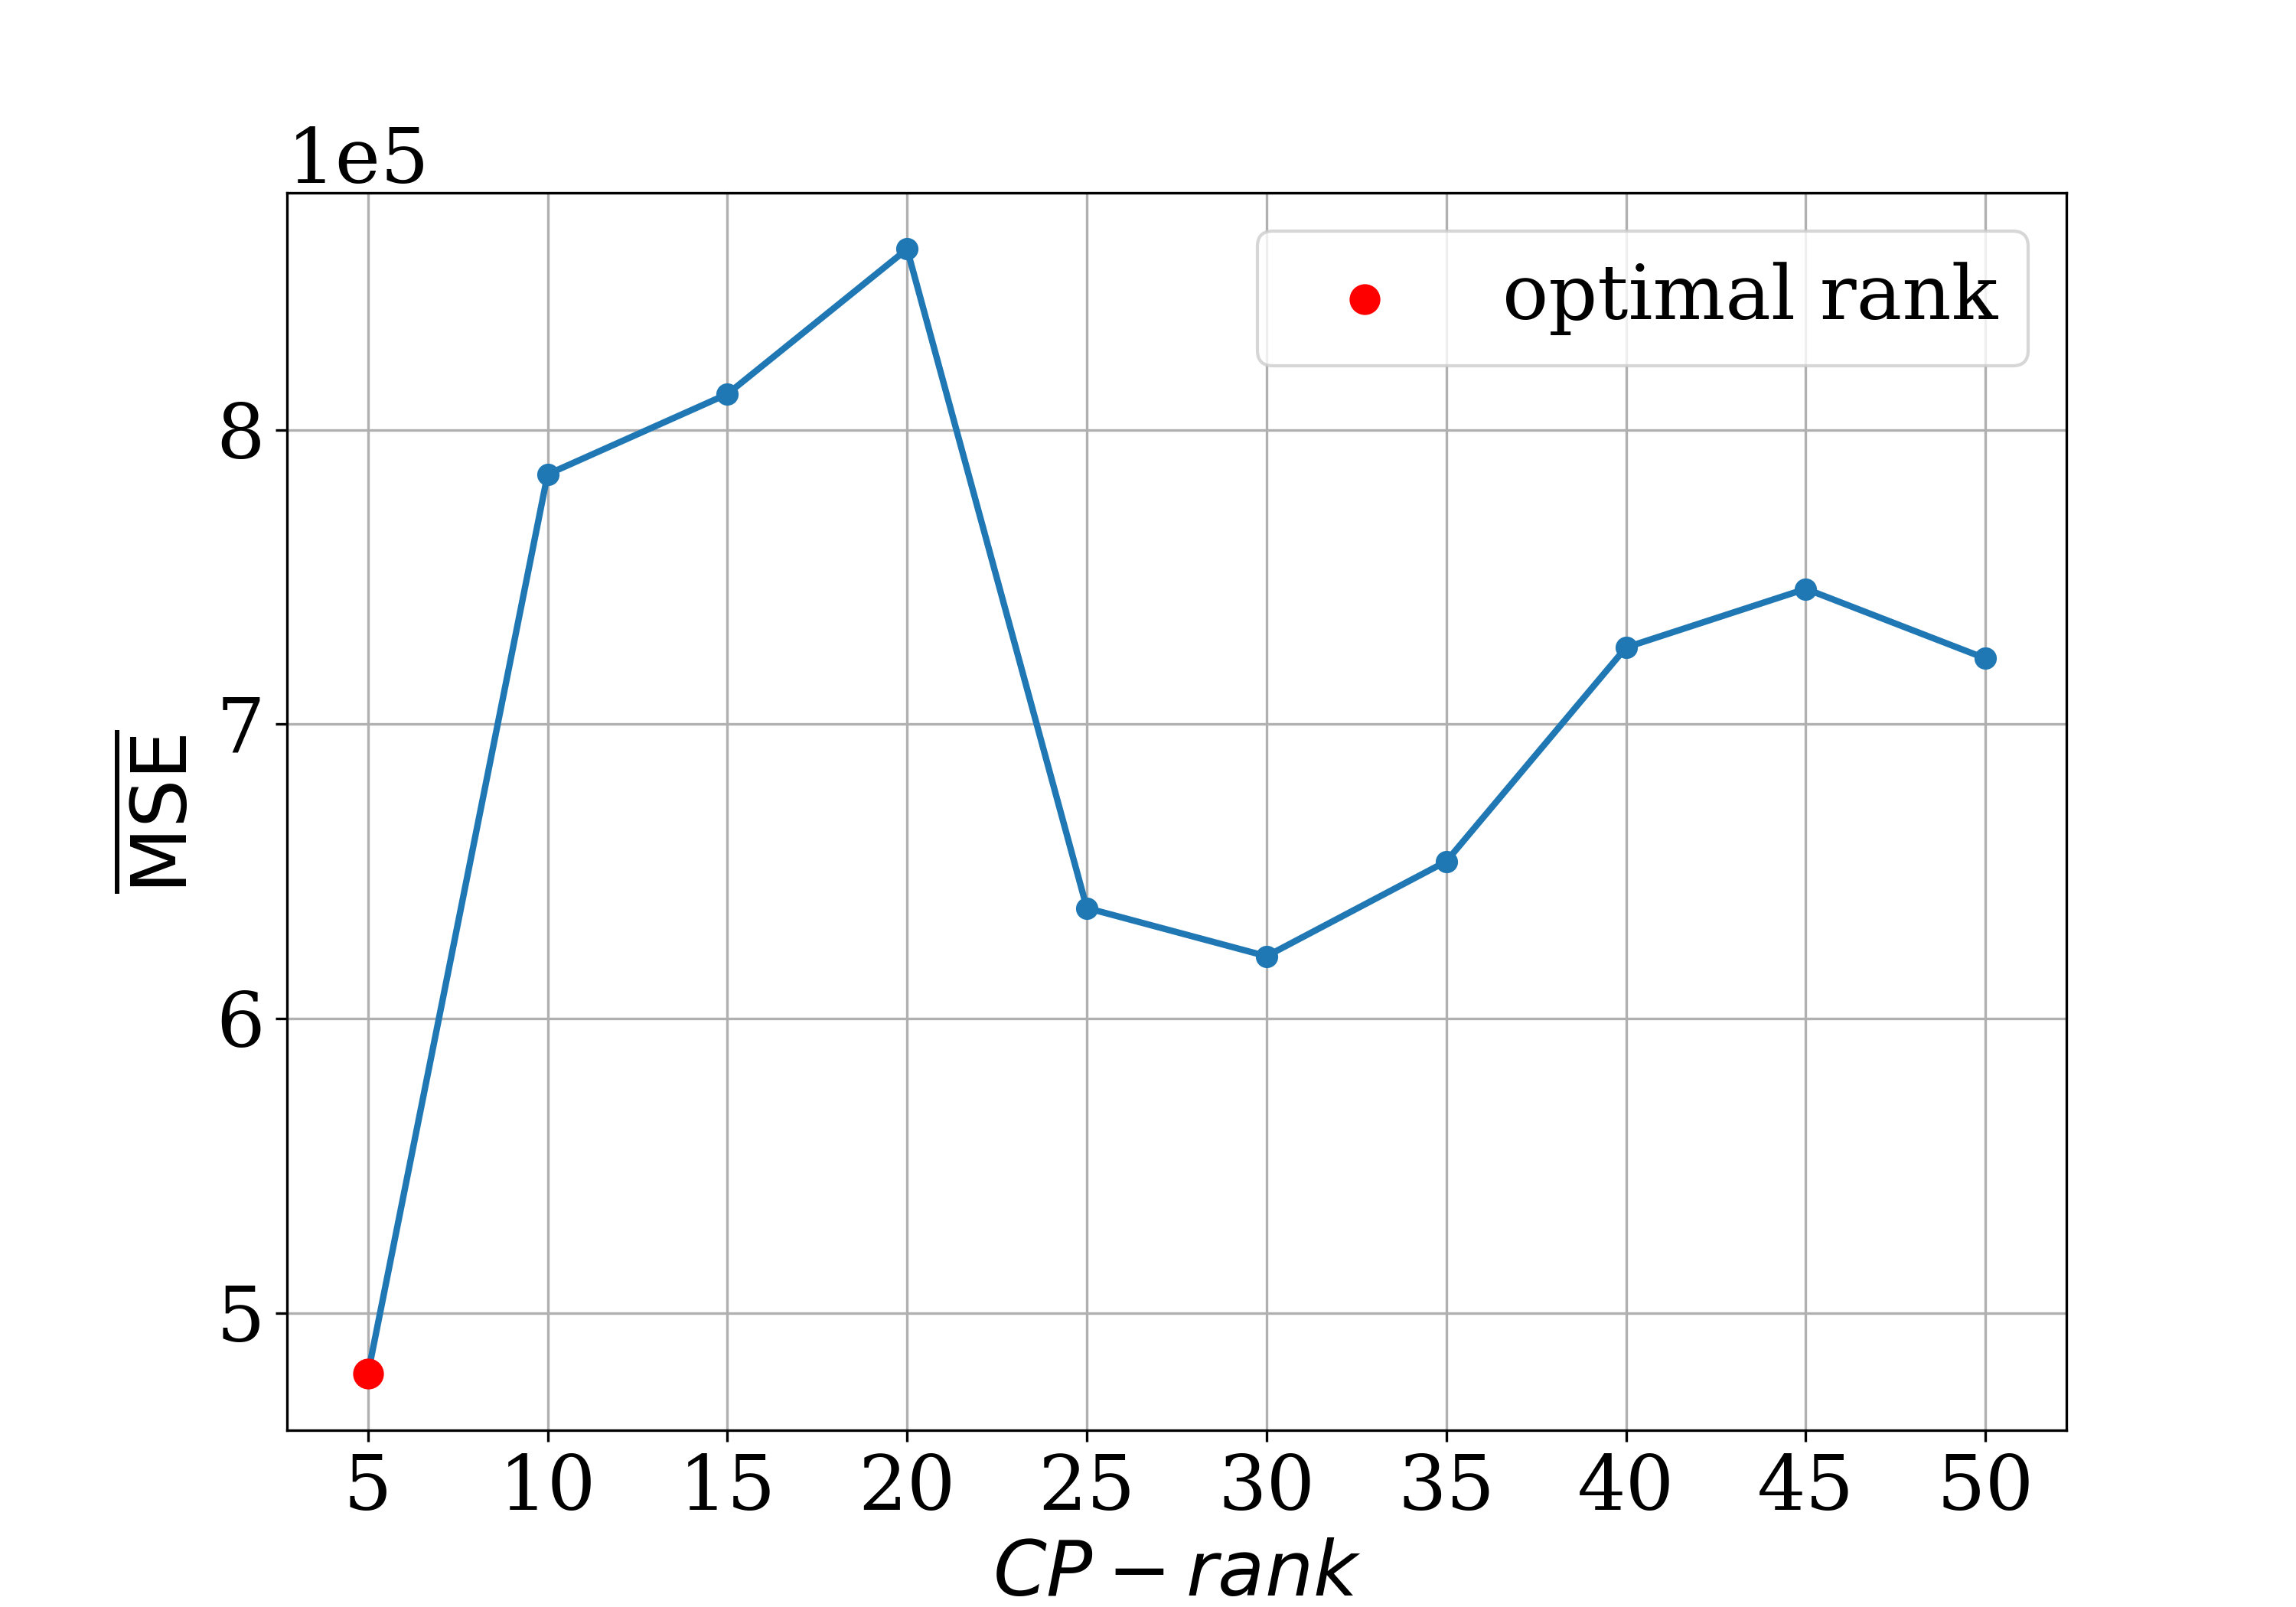
\includegraphics[width=0.48\textwidth, keepaspectratio]{pred_MSE_rank_elec.png}
		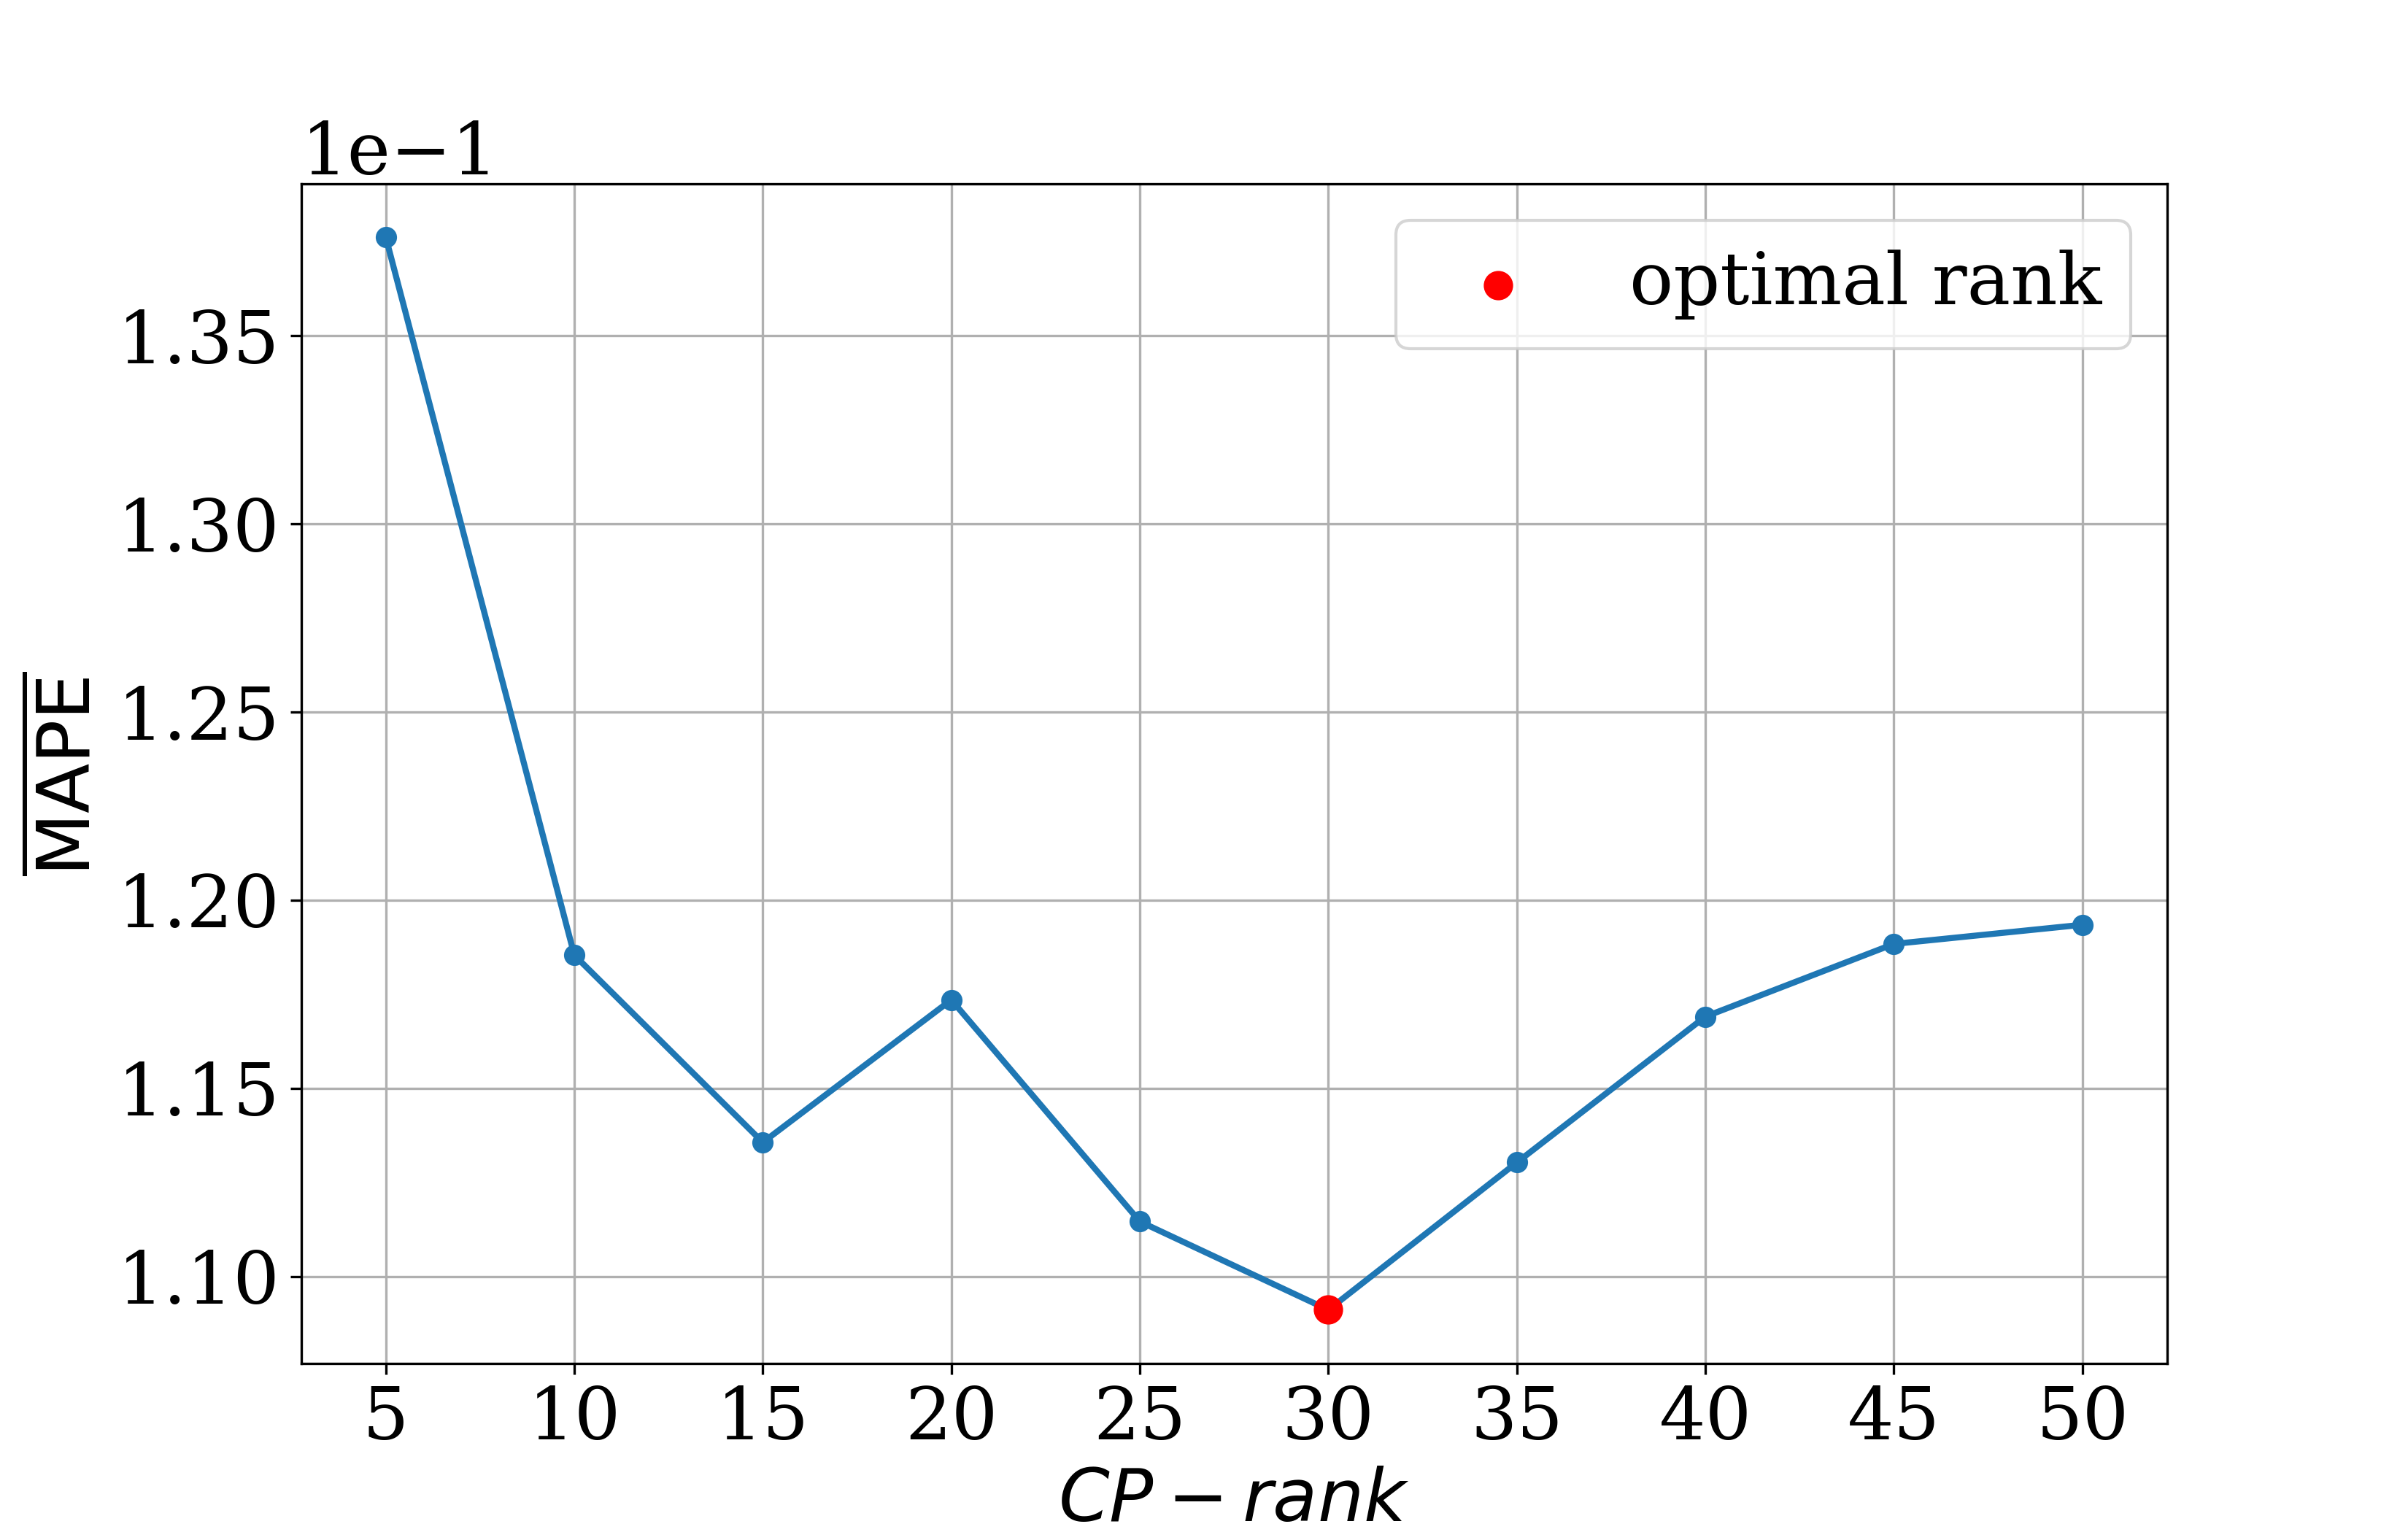
\includegraphics[width=0.48\textwidth, keepaspectratio]{pred_MAPE_rank_elec.png}
		\caption{$ \overline{\text{MSE}} $ and $ \overline{\text{MAPE}} $ metrics for the tSSA forecast depending on the CPD rank. An optimal point is marked with red. Electricity data.}\label{fig:mse_mape_electr}
	\end{figure}
	
	\begin{figure}[h]
		\centering
		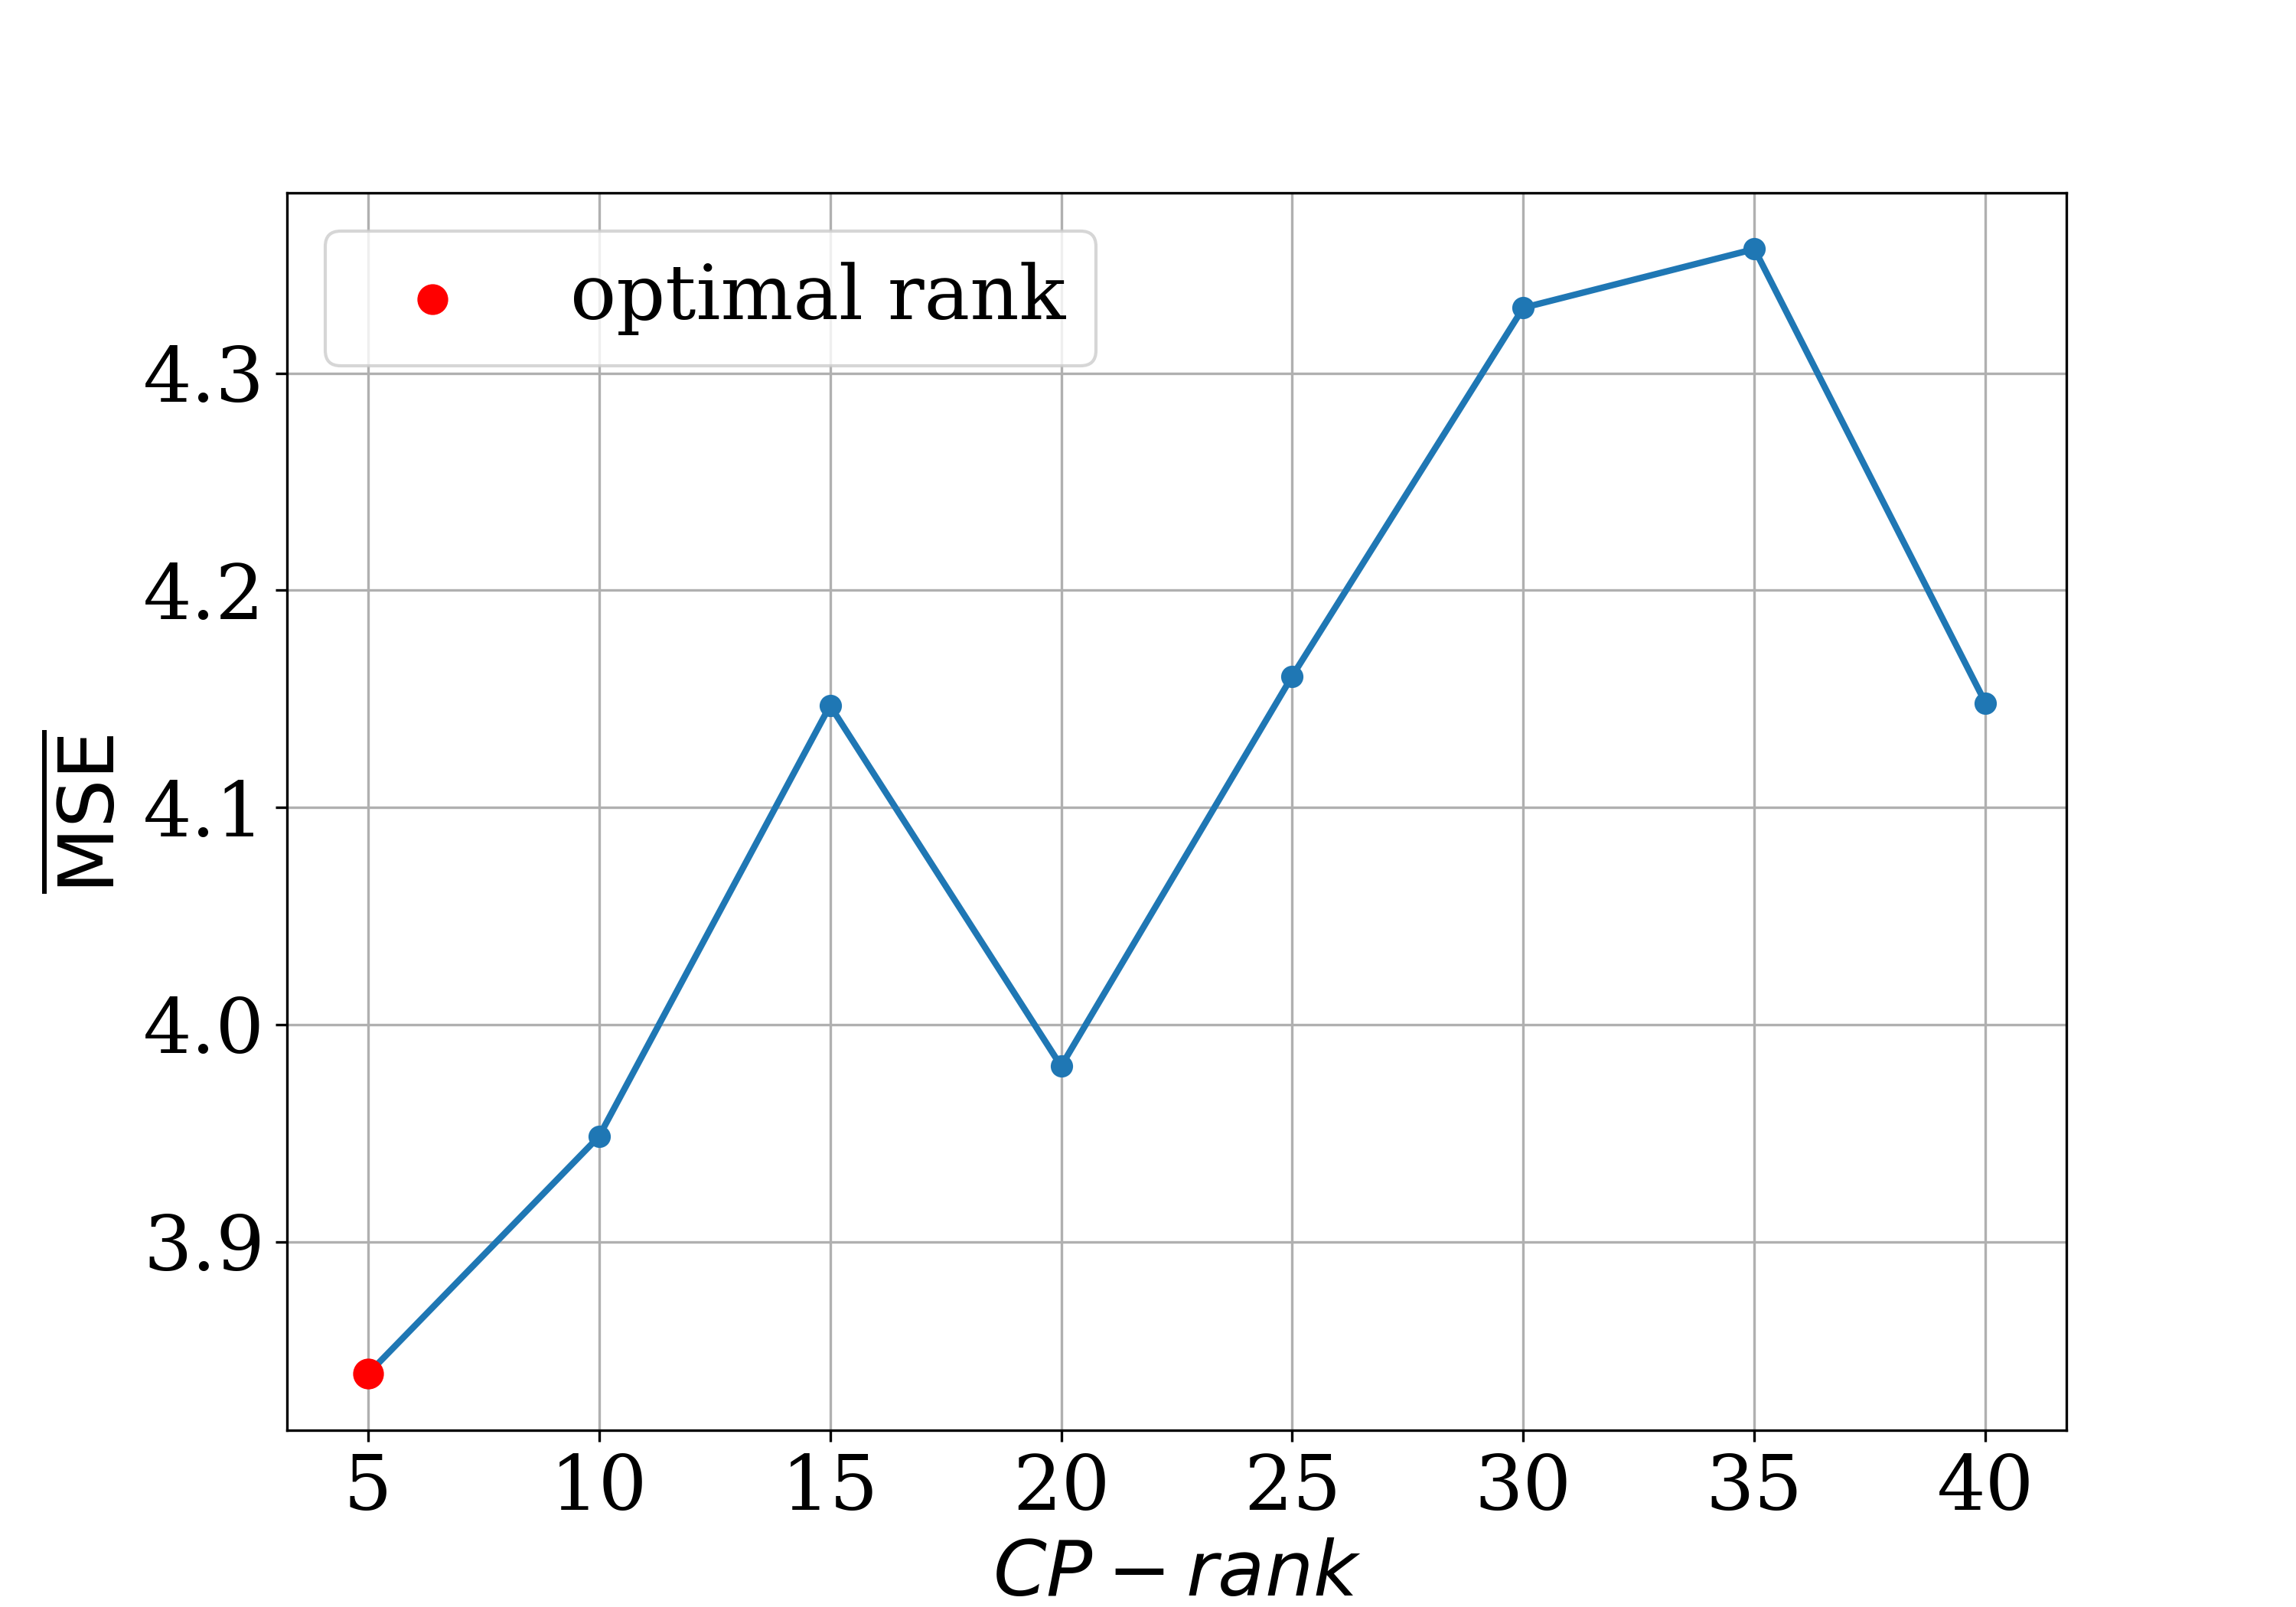
\includegraphics[width=0.48\textwidth, keepaspectratio]{pred_MSE_rank_motion.png}
		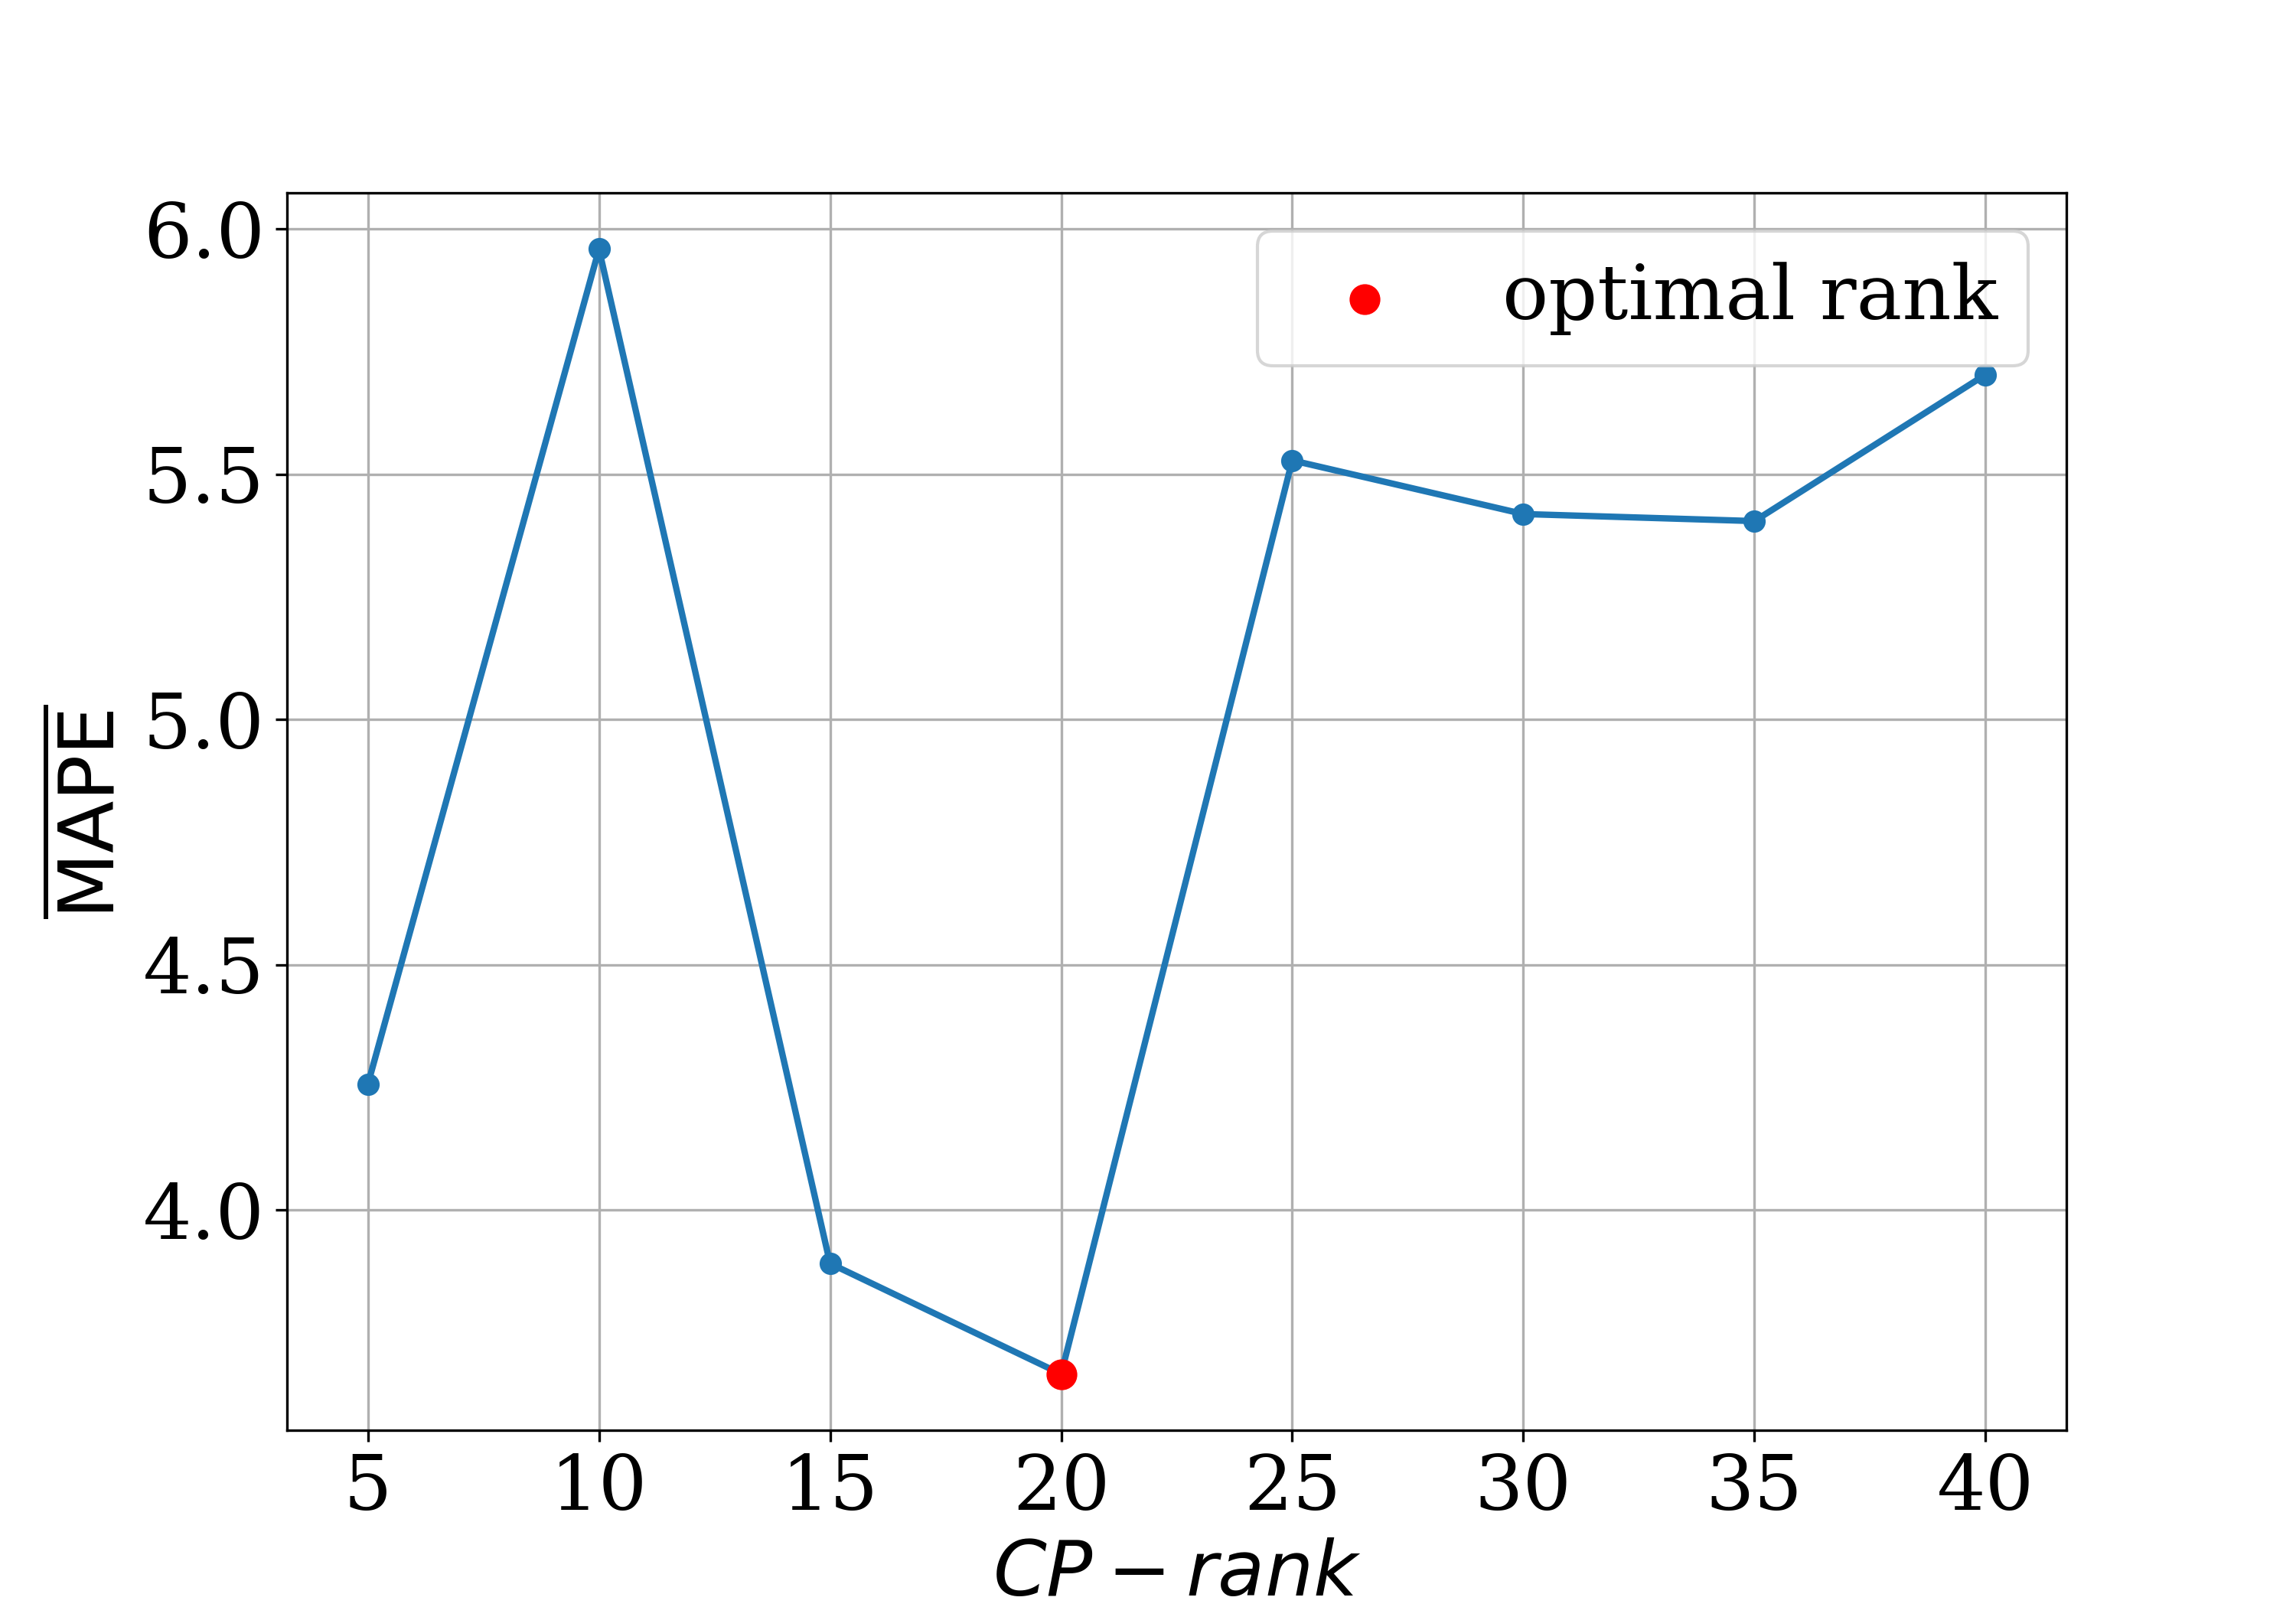
\includegraphics[width=0.48\textwidth, keepaspectratio]{pred_MAPE_rank_motion.png}
		\caption{$ \overline{\text{MSE}} $ and $ \overline{\text{MAPE}} $ metrics for the tSSA forecast depending on the CPD rank. An optimal point is marked with red. Inertial unit data.}\label{fig:mse_mape_motion}
	\end{figure}
	
	\begin{figure}[h]
		\centering
		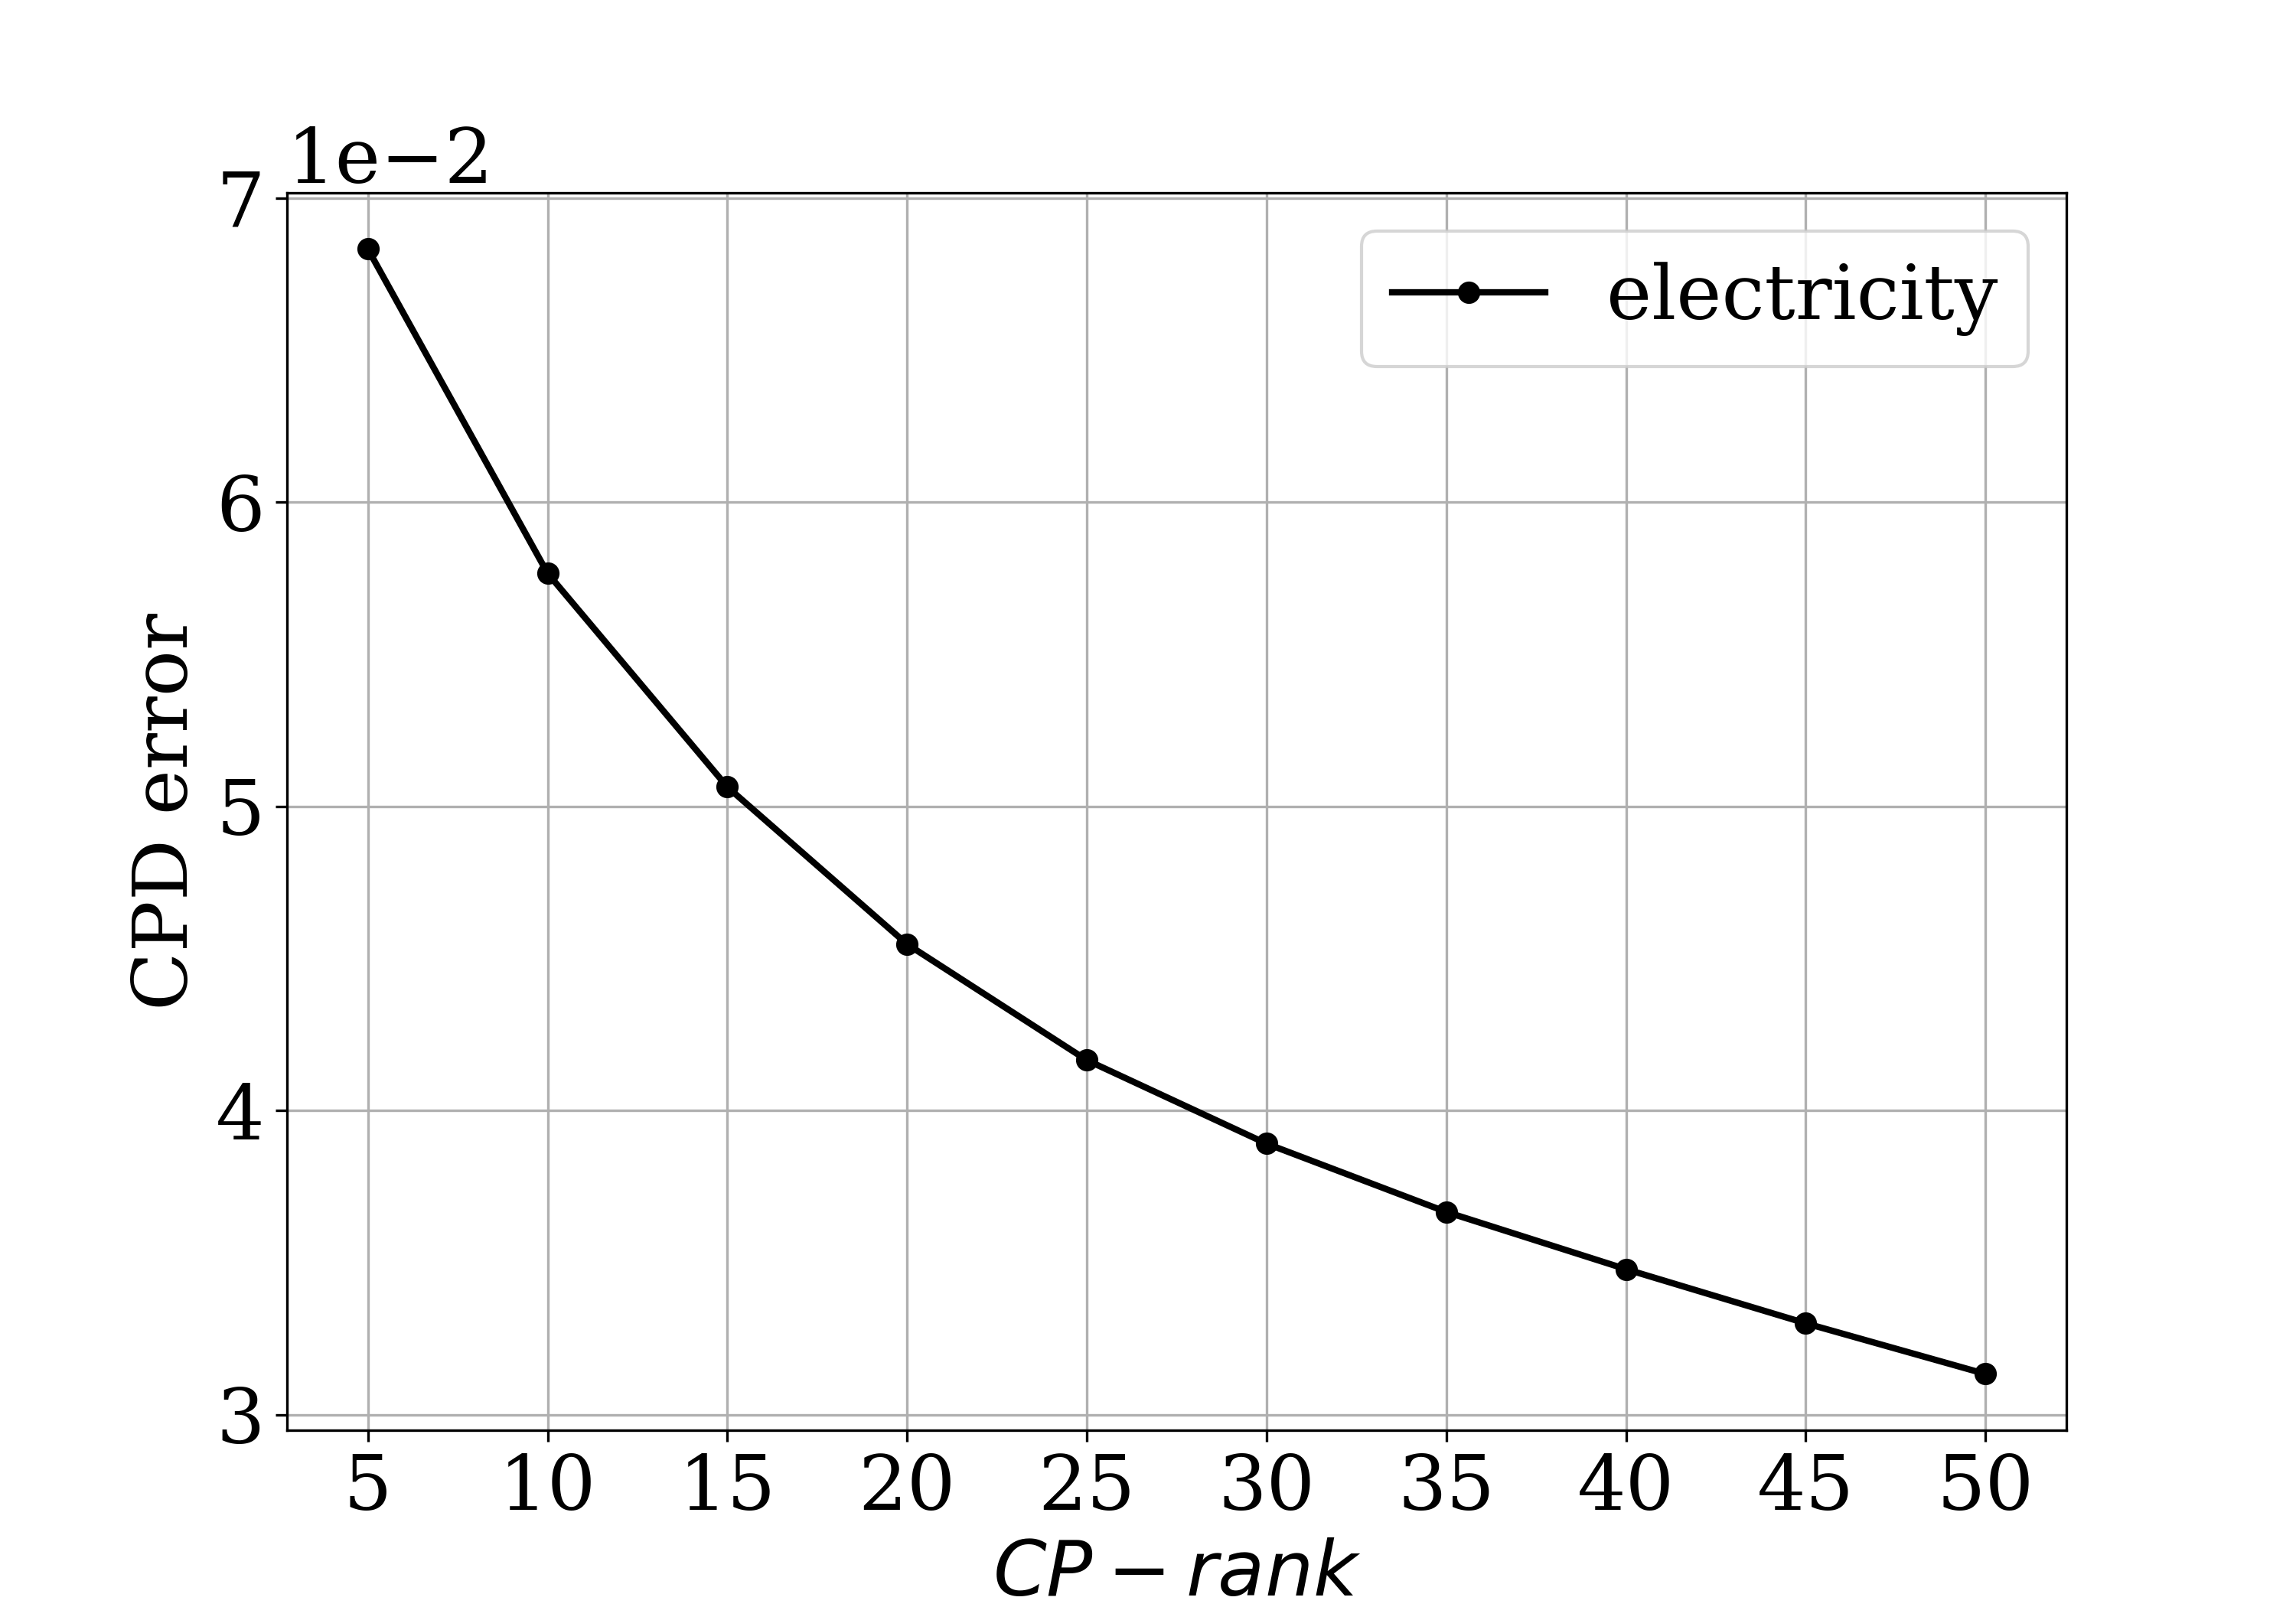
\includegraphics[width=0.48\textwidth, keepaspectratio]{CPD_error_elec.png}
		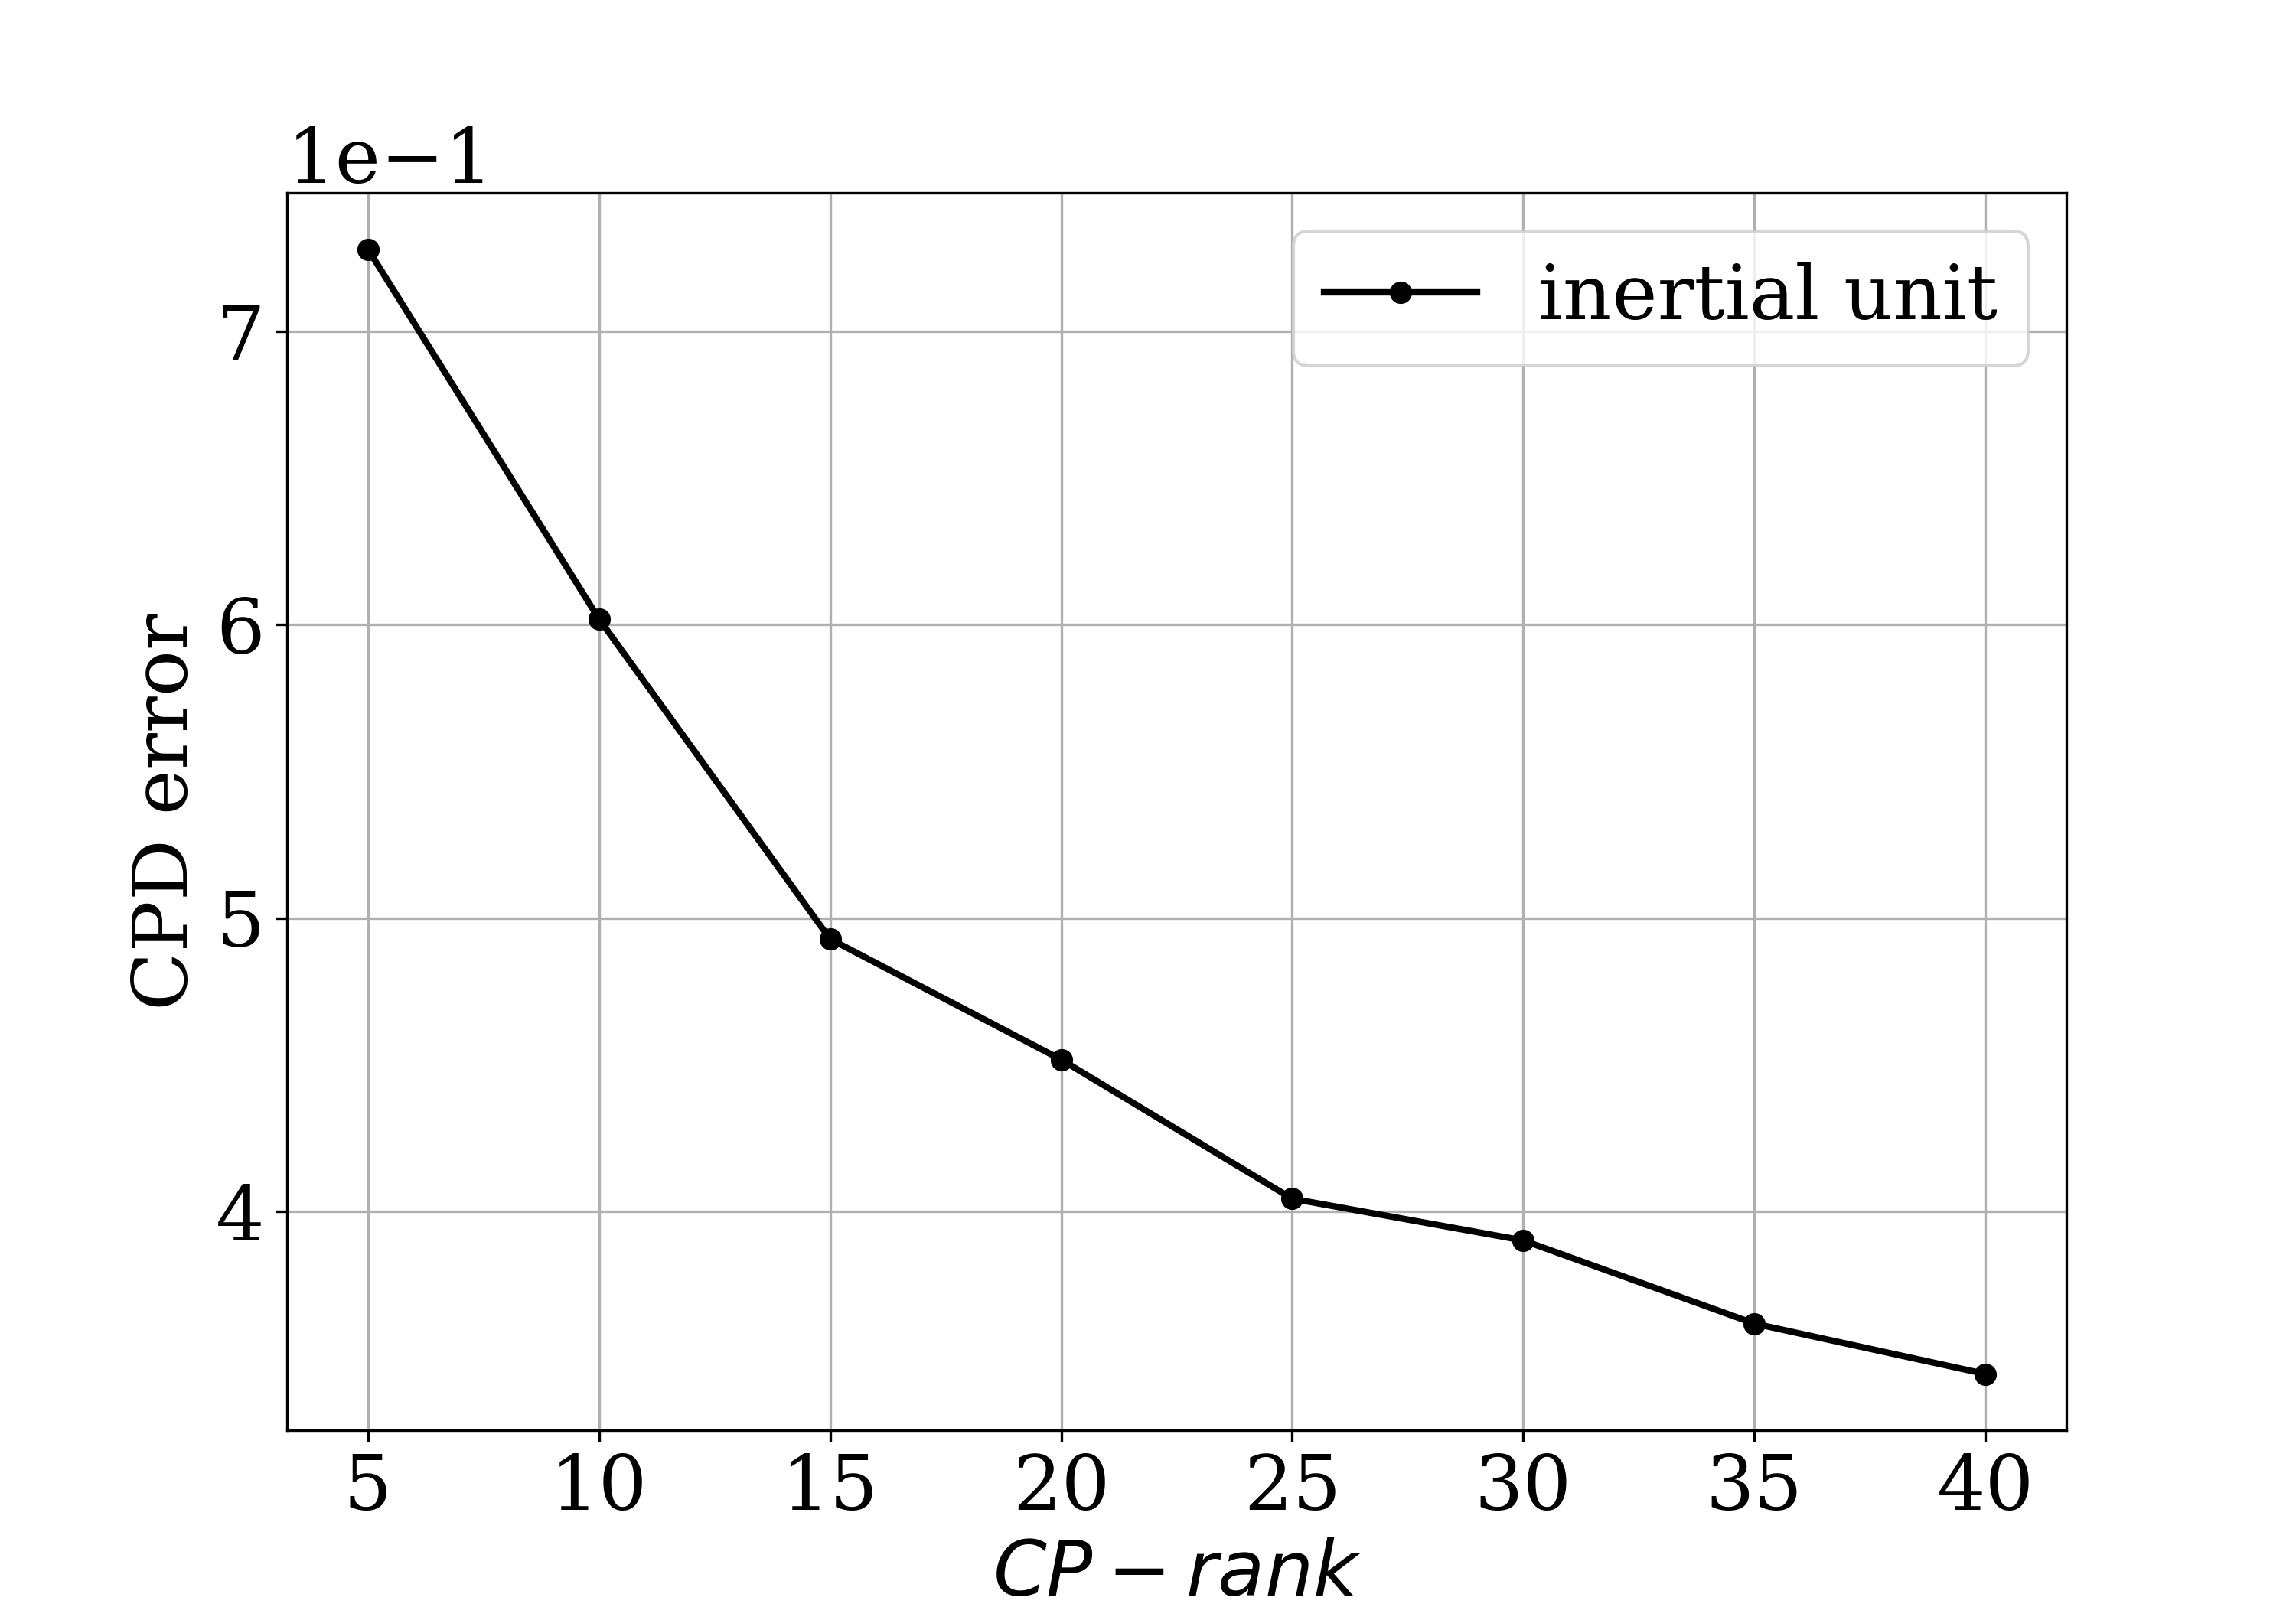
\includegraphics[width=0.48\textwidth, keepaspectratio]{CPD_error_motion.png}
		\caption{Relative CPD approximation errors depending on the CPD rank. The left is for the electricity data, the right is for the inertial unit data.}\label{fig:cpd_errors}
	\end{figure}
	
	The best tSSA forecast is shown in the Fig. \ref{fig:tssa_electr_pred} and \ref{fig:tssa_motion_pred}. For electricity, the CPD rank is rather big. Therefore, the order of the forecast model (see Sec. \ref{sec:tssa_forecast}) is high. The resulting forecast approximates test data quite accurately. On the other hand, big rank for the inertial unit data lead to the unstable and unbound forecast. With the smaller rank, model is more accurate. However, the forecast model's order is decreased. Consequently, the build forecast approximates only mean values.
	
	\begin{figure}[h]
		\centering
		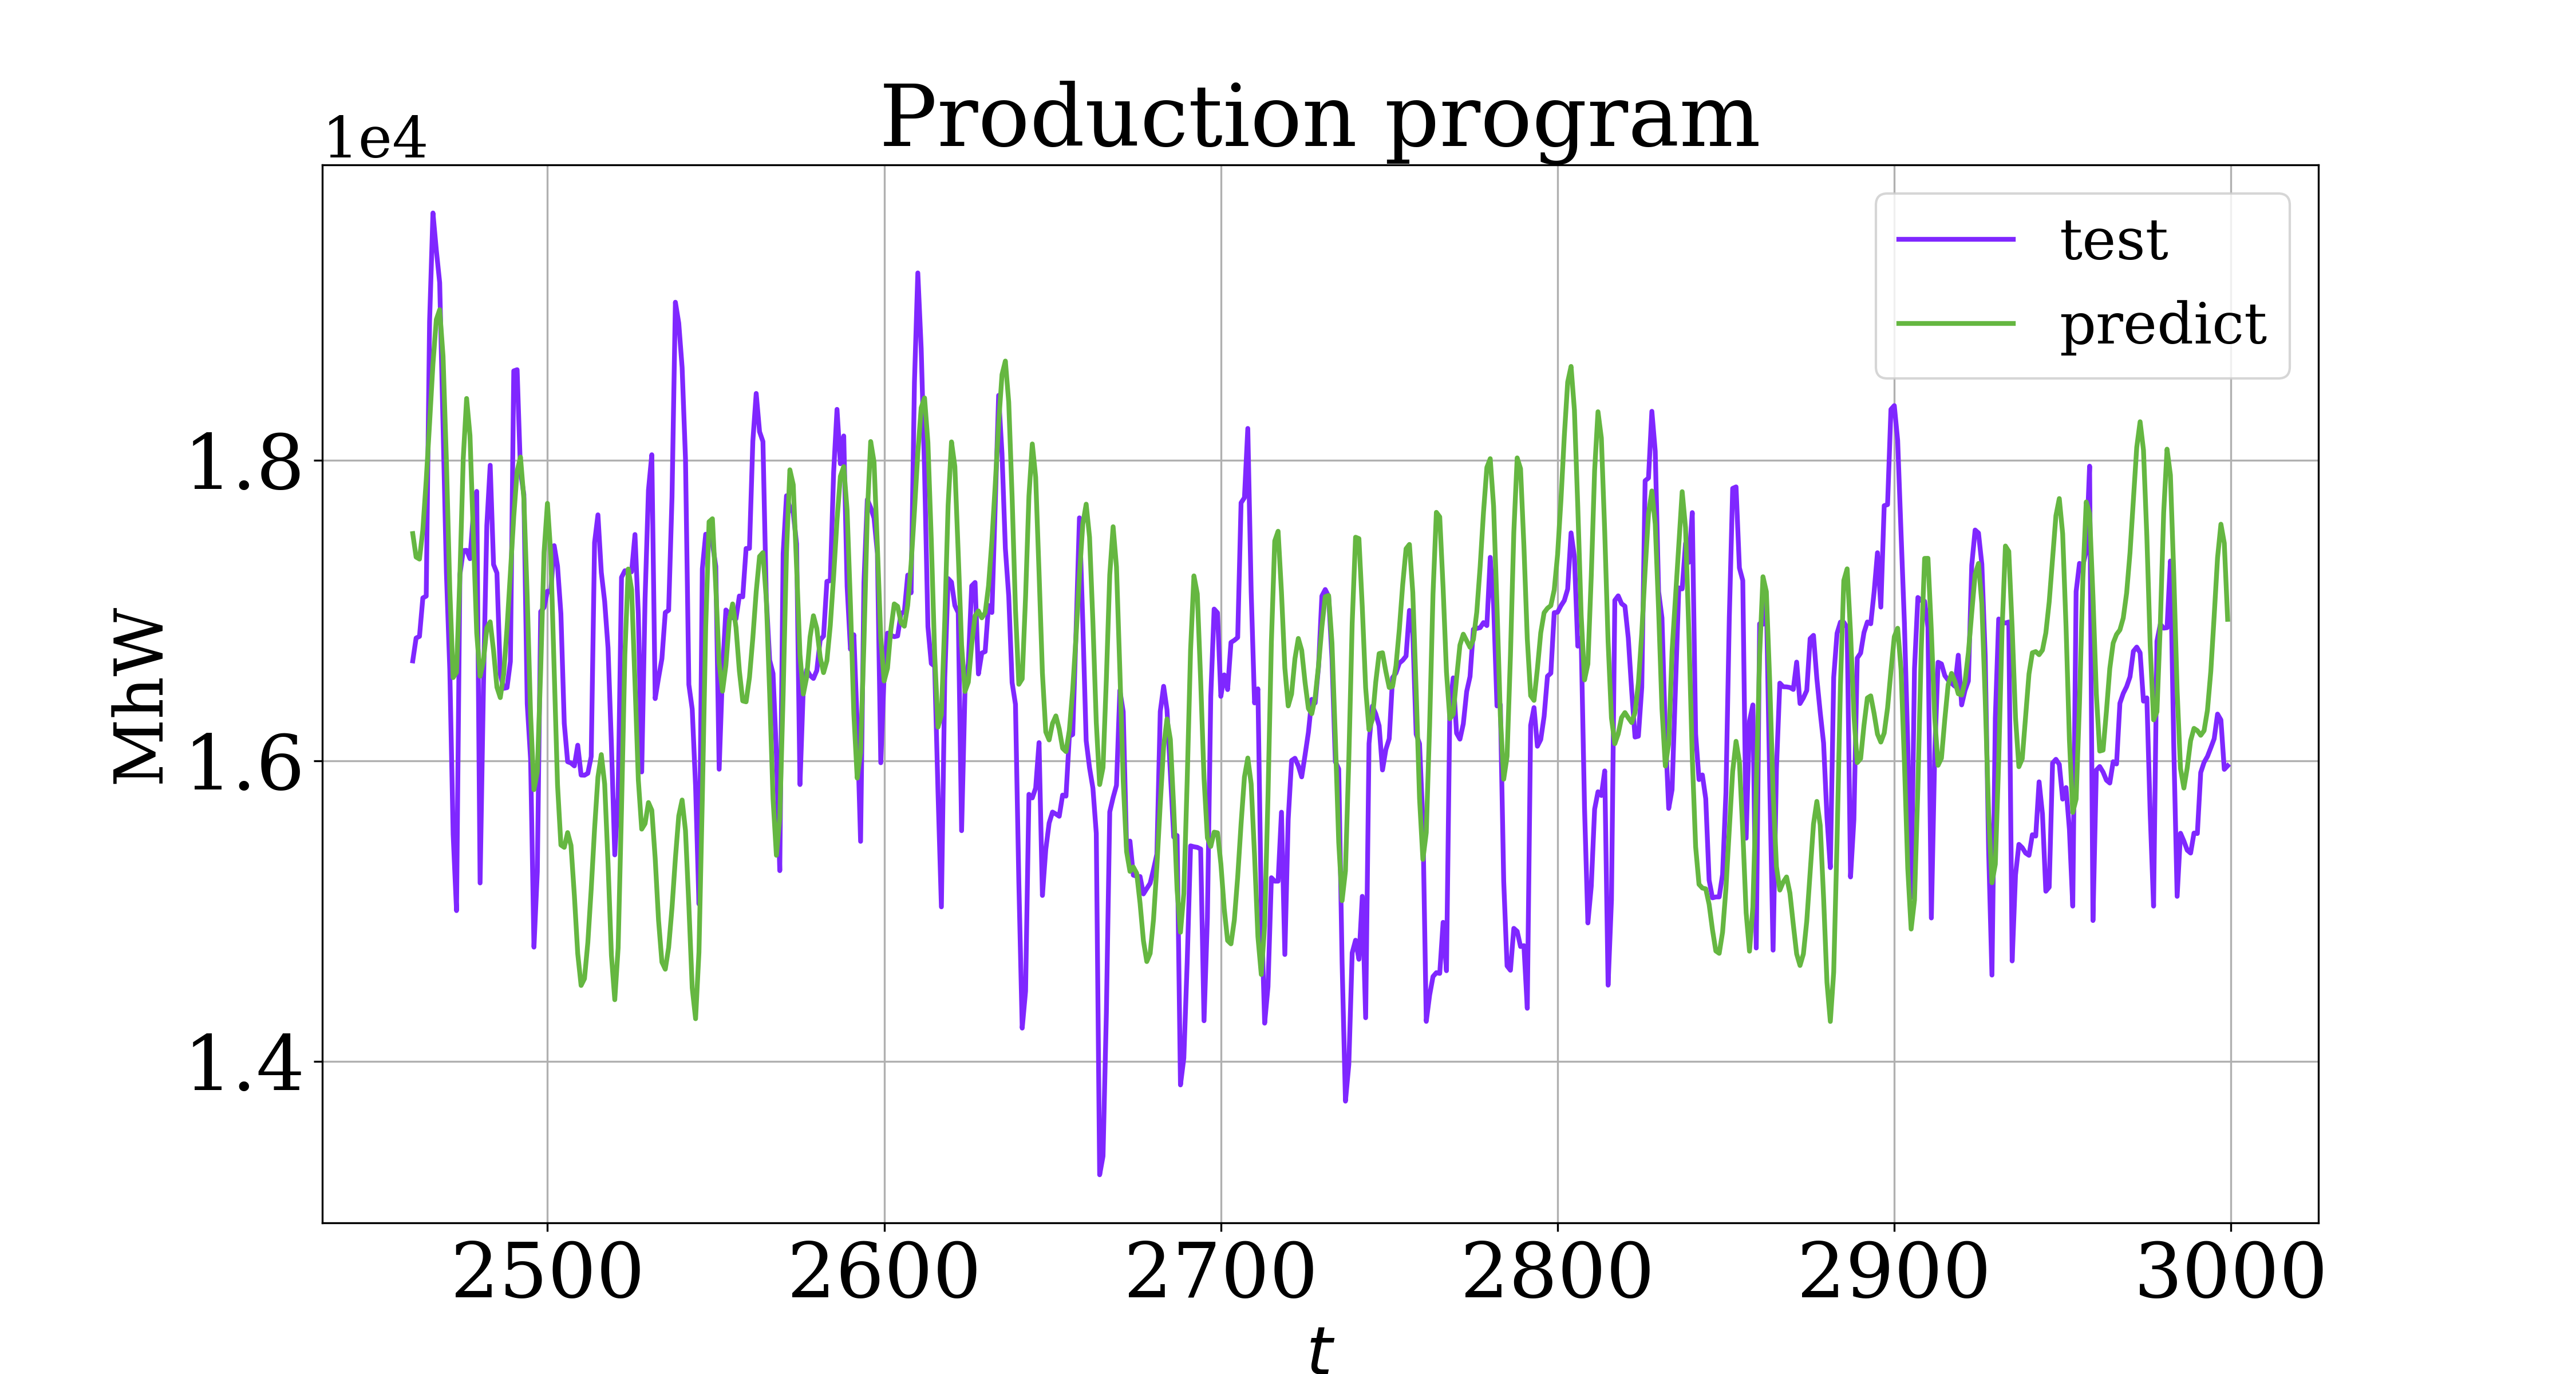
\includegraphics[width=0.48\textwidth, keepaspectratio]{Production_program_pred.png}
		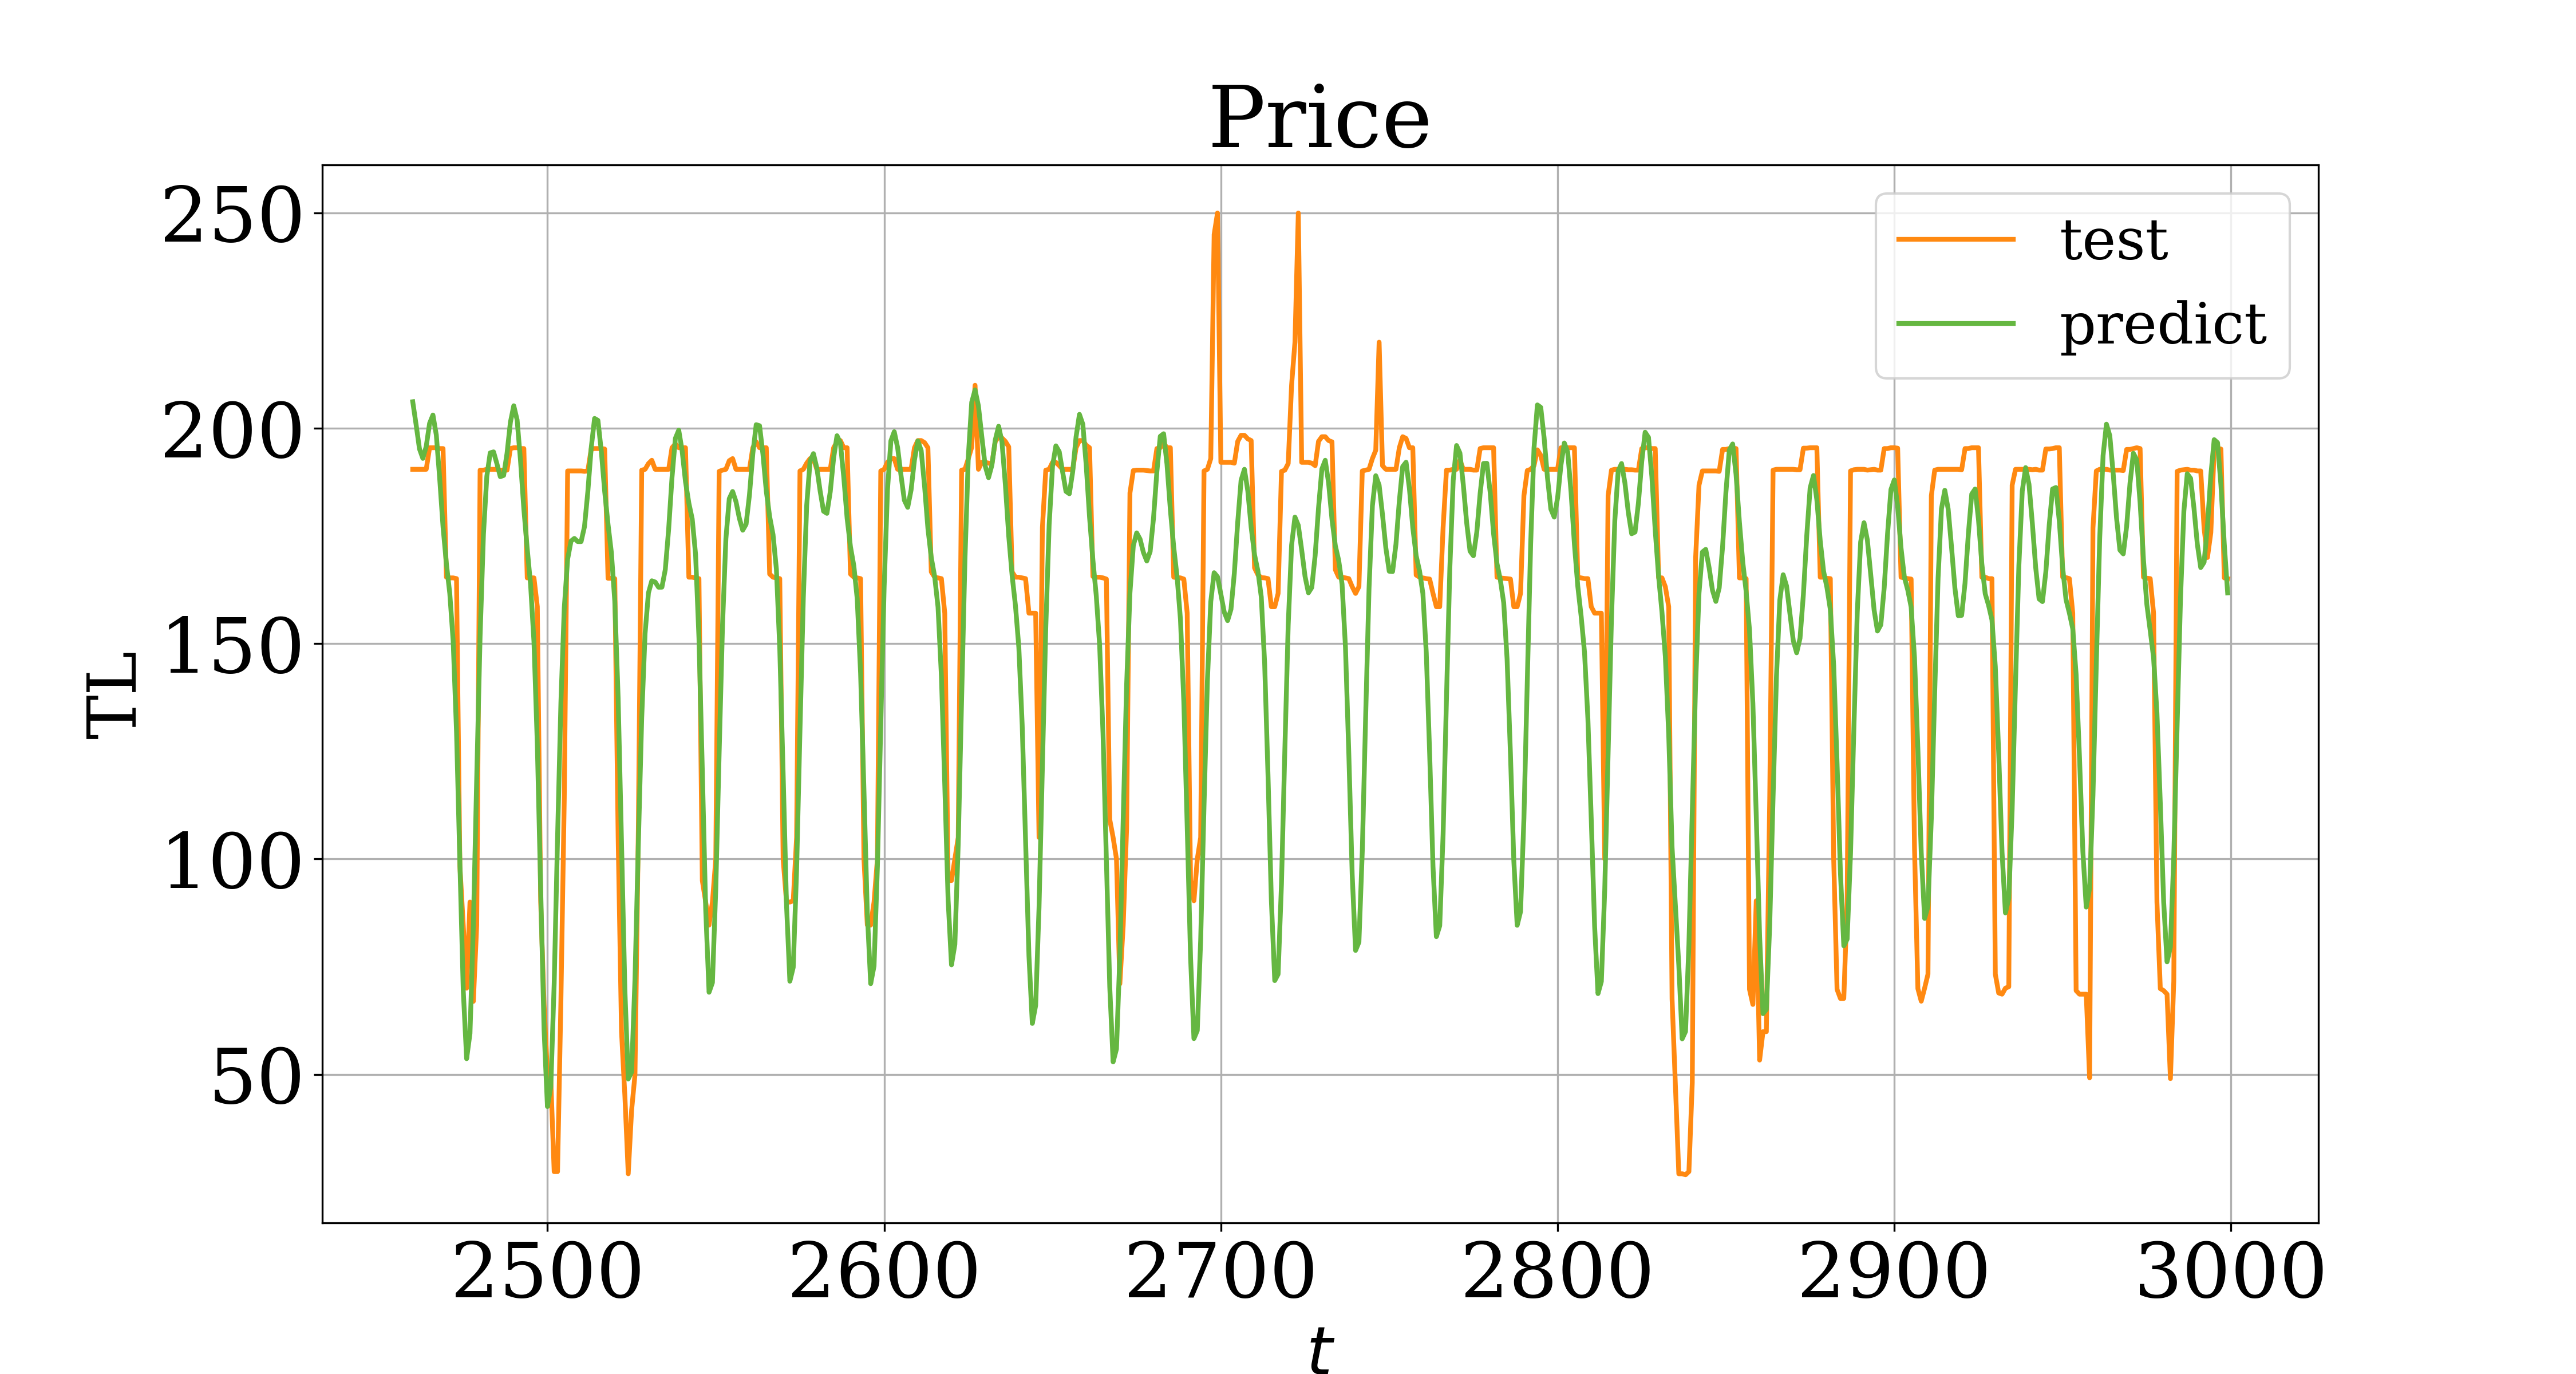
\includegraphics[width=0.48\textwidth, keepaspectratio]{Price_pred.png}
		\caption{tSSA forecast for the electricity data. The CPD rank $ = 30 $}\label{fig:tssa_electr_pred}
	\end{figure}
	
	\begin{figure}[h]
		\centering
		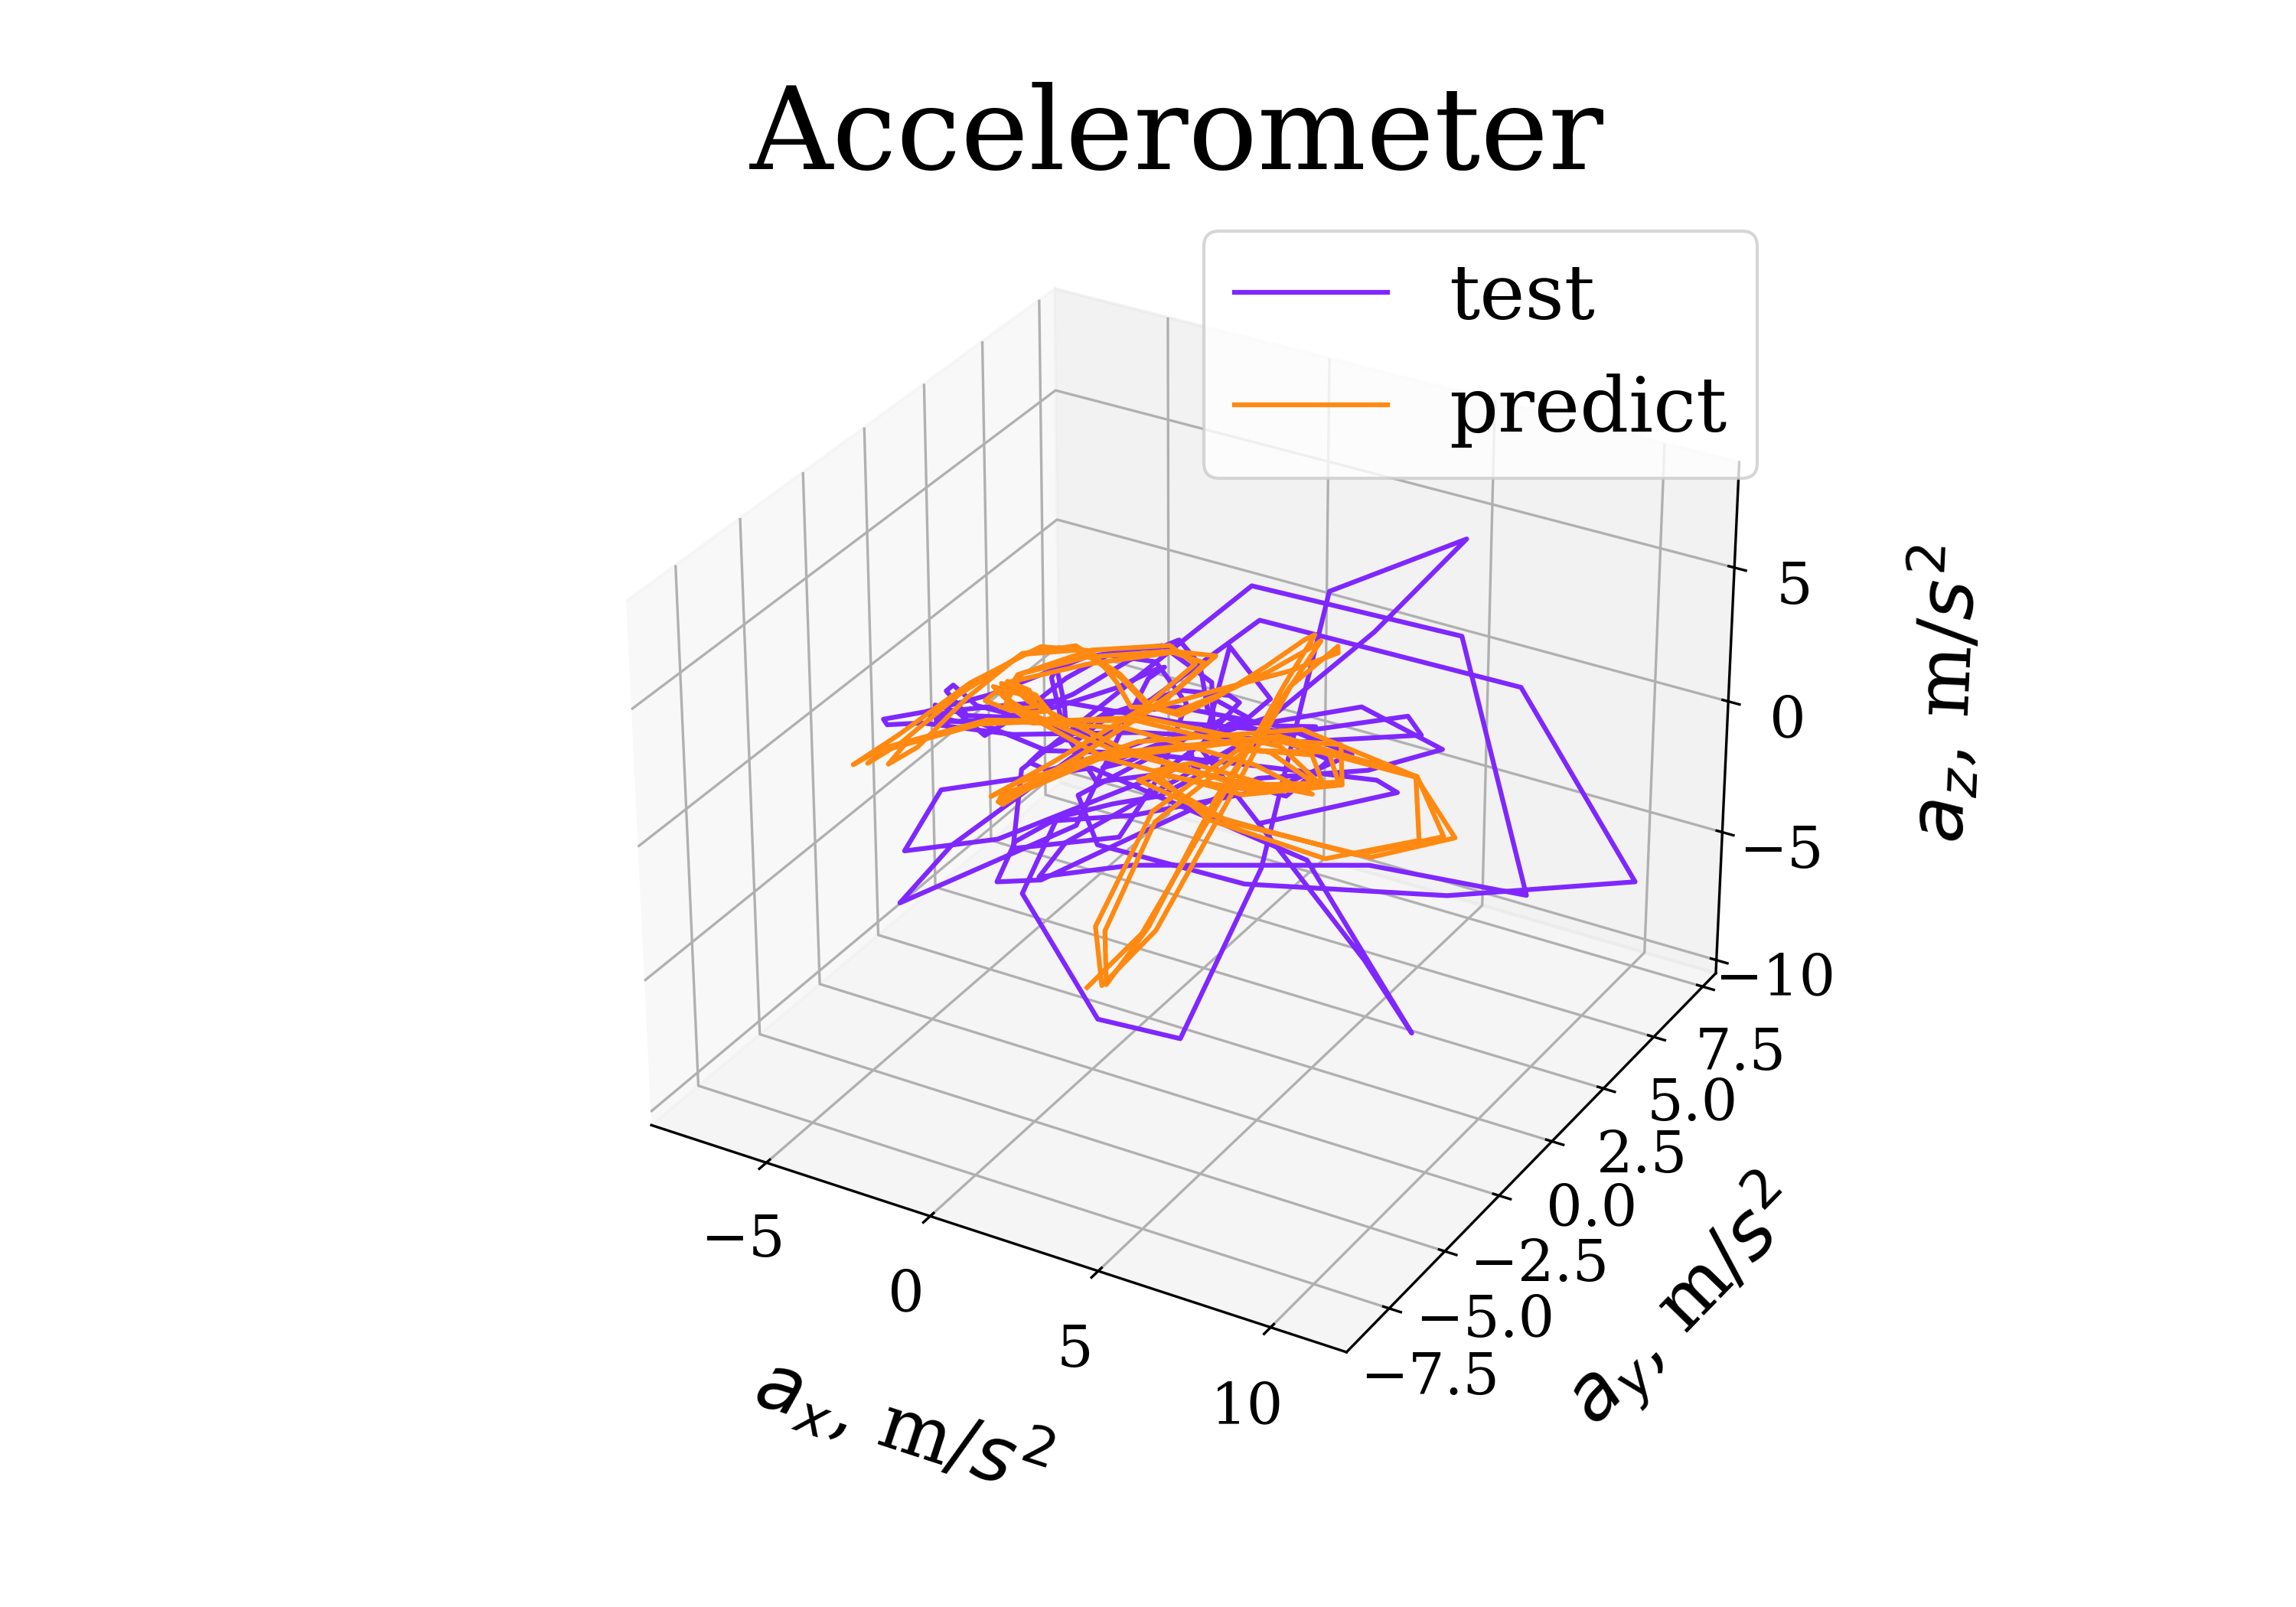
\includegraphics[width=0.48\textwidth, keepaspectratio]{acceler_pred.png}
		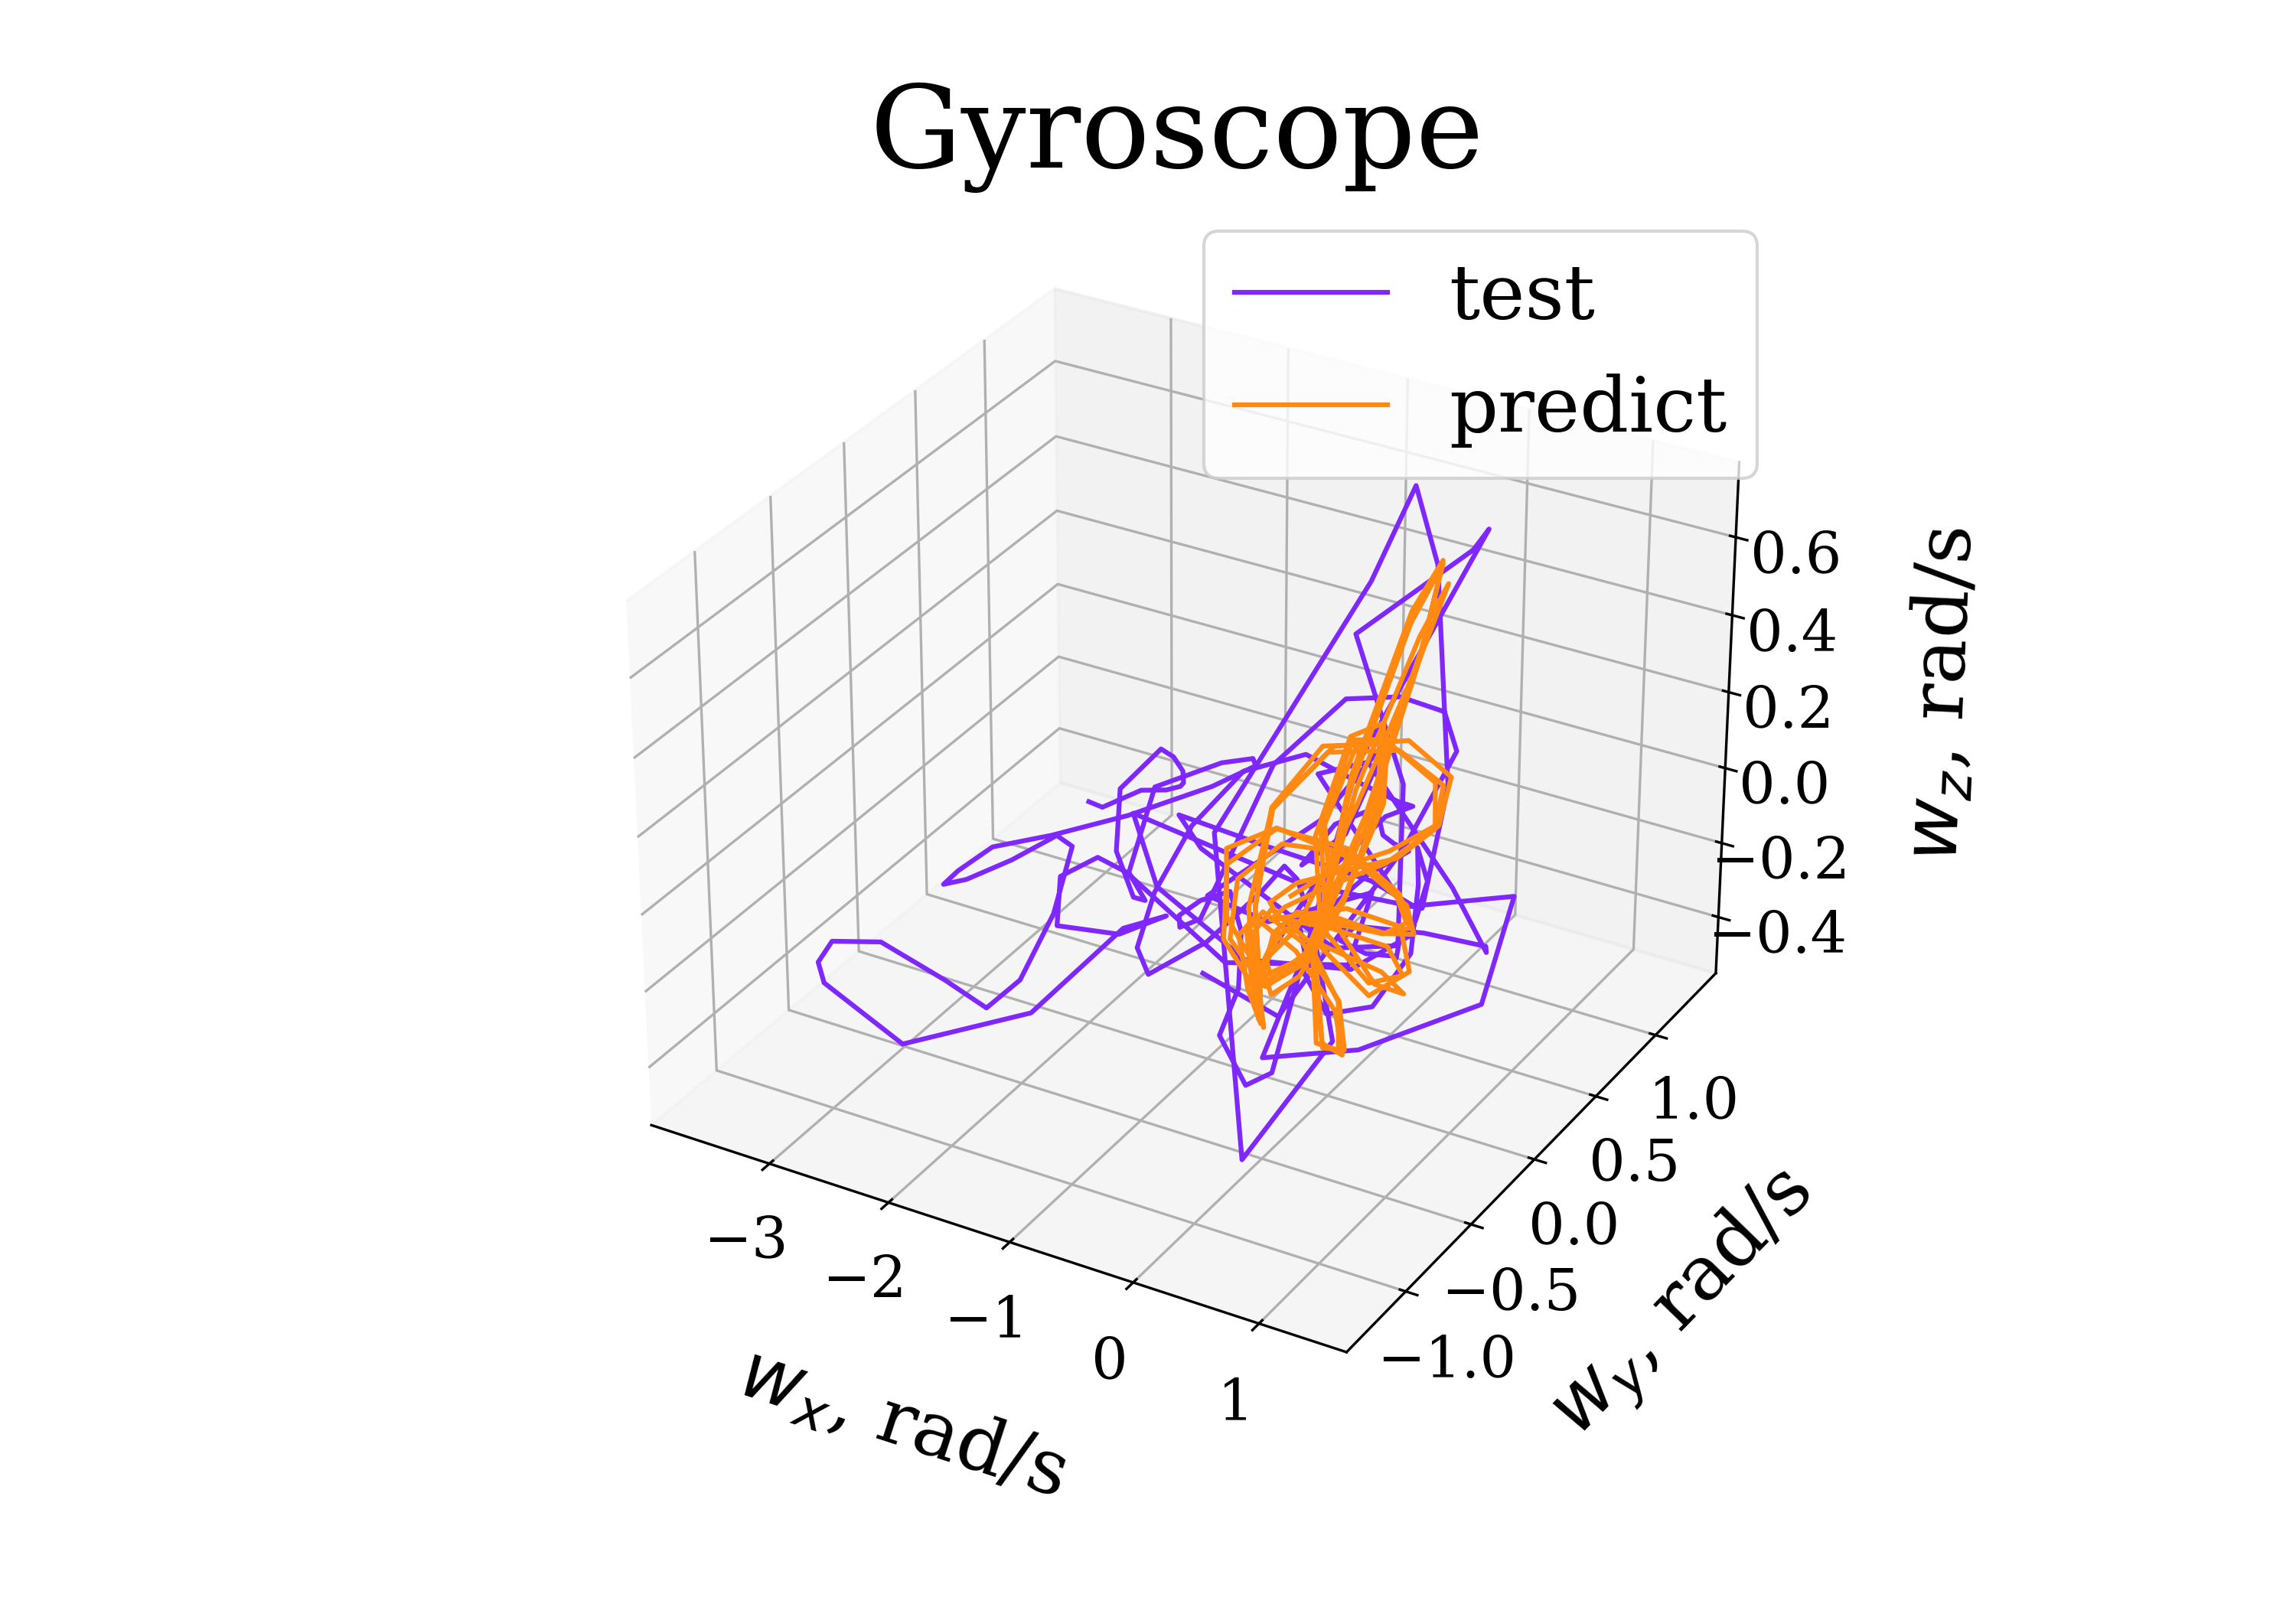
\includegraphics[width=0.48\textwidth, keepaspectratio]{gyro_pred.png}
		\caption{tSSA forecast for the inertial unit data. The CPD rank $ = 20 $}\label{fig:tssa_motion_pred}
	\end{figure}
	
	The forecast metrics for all models are in the Tab. \ref{tab:pred_res_electr} and \ref{tab:pred_res_motion}. Our method showed the best results in most cases. Close values were obtained with the mSSA. The VAR model appeared unstable for the chosen forecast test data. The RNN was able to learn only the constant function from the electricity data. But with the greater $ L $ for the inertial unit data, the RNN performed better.
	
	\def\arraystretch{1.2}
	\begin{table}[h]
		\centering
		\caption{Prediction quality of the models on the electricity data}\label{tab:pred_res_electr}
		\begin{tabular}{|c|c|c|c|c|}
			\hline
			& \textit{tSSA}  & \textit{mSSA} & \textit{VAR} & \textit{RNN} \\ \hline
			$ \overline{\text{MSE}}_{\text{Producution}} $, $10^6$ & 1.24           & 1.51          & 7.81         & 2.70         \\ \hline
			$ \overline{\text{MSE}}_{\text{Price}} $, $10^3$      & 0.88           & 1.03          & 4.85         & 30.0         \\ \hline
			$ \overline{\text{MSE}} $, $10^6$             & \textbf{0.62}  & 0.75          & 3.91         & 135.00       \\ \hline
			$ \overline{\text{MAPE}}_{\text{Producution}} $        & 0.054          & 0.060         & 0.137        & 0.999        \\ \hline
			$ \overline{\text{MAPE}}_{\text{Price}} $             & 0.164          & 0.170         & 0.360        & 1.004        \\ \hline
			$ \overline{\text{MAPE}} $                    & \textbf{0.109} & 0.115         & 0.249        & 1.002        \\ \hline
		\end{tabular}
	\end{table}
	
	\def\arraystretch{1.2}
	\begin{table}[h]
		\centering
		\caption{Prediction quality of the models on the inertial unit data}\label{tab:pred_res_motion}
		\begin{tabular}{|c|c|c|c|c|}
			\hline
			& \textit{tSSA}                & \textit{mSSA} & \textit{VAR} & \textit{RNN} \\ \hline
			$ \overline{\text{MSE}}_{\text{Accel}} $  & 7.351          & 6.980 & 8.108  & 6.604          \\ \hline
			$ \overline{\text{MSE}}_{\text{Gyro}} $   & 0.610          & 0.636 & 0.631  & 0.639          \\ \hline
			$ \overline{\text{MSE}} $         & 3.981          & 3.808 & 4.370  & \textbf{3.622} \\ \hline
			$ \overline{\text{MAPE}}_{\text{Accel}} $ & 3.558          & 3.516 & 3.370  & 1.747          \\ \hline
			$ \overline{\text{MAPE}}_{\text{Gyro}} $  & 3.773          & 3.943 & 10.427 & 5.641          \\ \hline
			$ \overline{\text{MAPE}} $        & \textbf{3.666} & 3.730 & 6.899  & 3.694          \\ \hline
		\end{tabular}
	\end{table}
	
	Now we move to the decomposition results. The Fig. \ref{fig:decomp_rhe_rank} illustrates relationship between the quality metrics and the CPD rank. In both cases the $ \overline{\text{RHE}} $ rapidly reaches a minimum and then does not change or even increase. Recalling the same result for the forecast, we can conclude that the tSSA has the greatest generalization capacity for the small tensor ranks. At the same time, the rank is a value of the shared phase space dimension (see Sec. \ref{sec:tssa_method}). Therefore, the tSSA finds a low dimensional data representation as was indicated in the Sec. \ref{sec:problem_statement}.
	
	\begin{figure}[h]
		\centering
		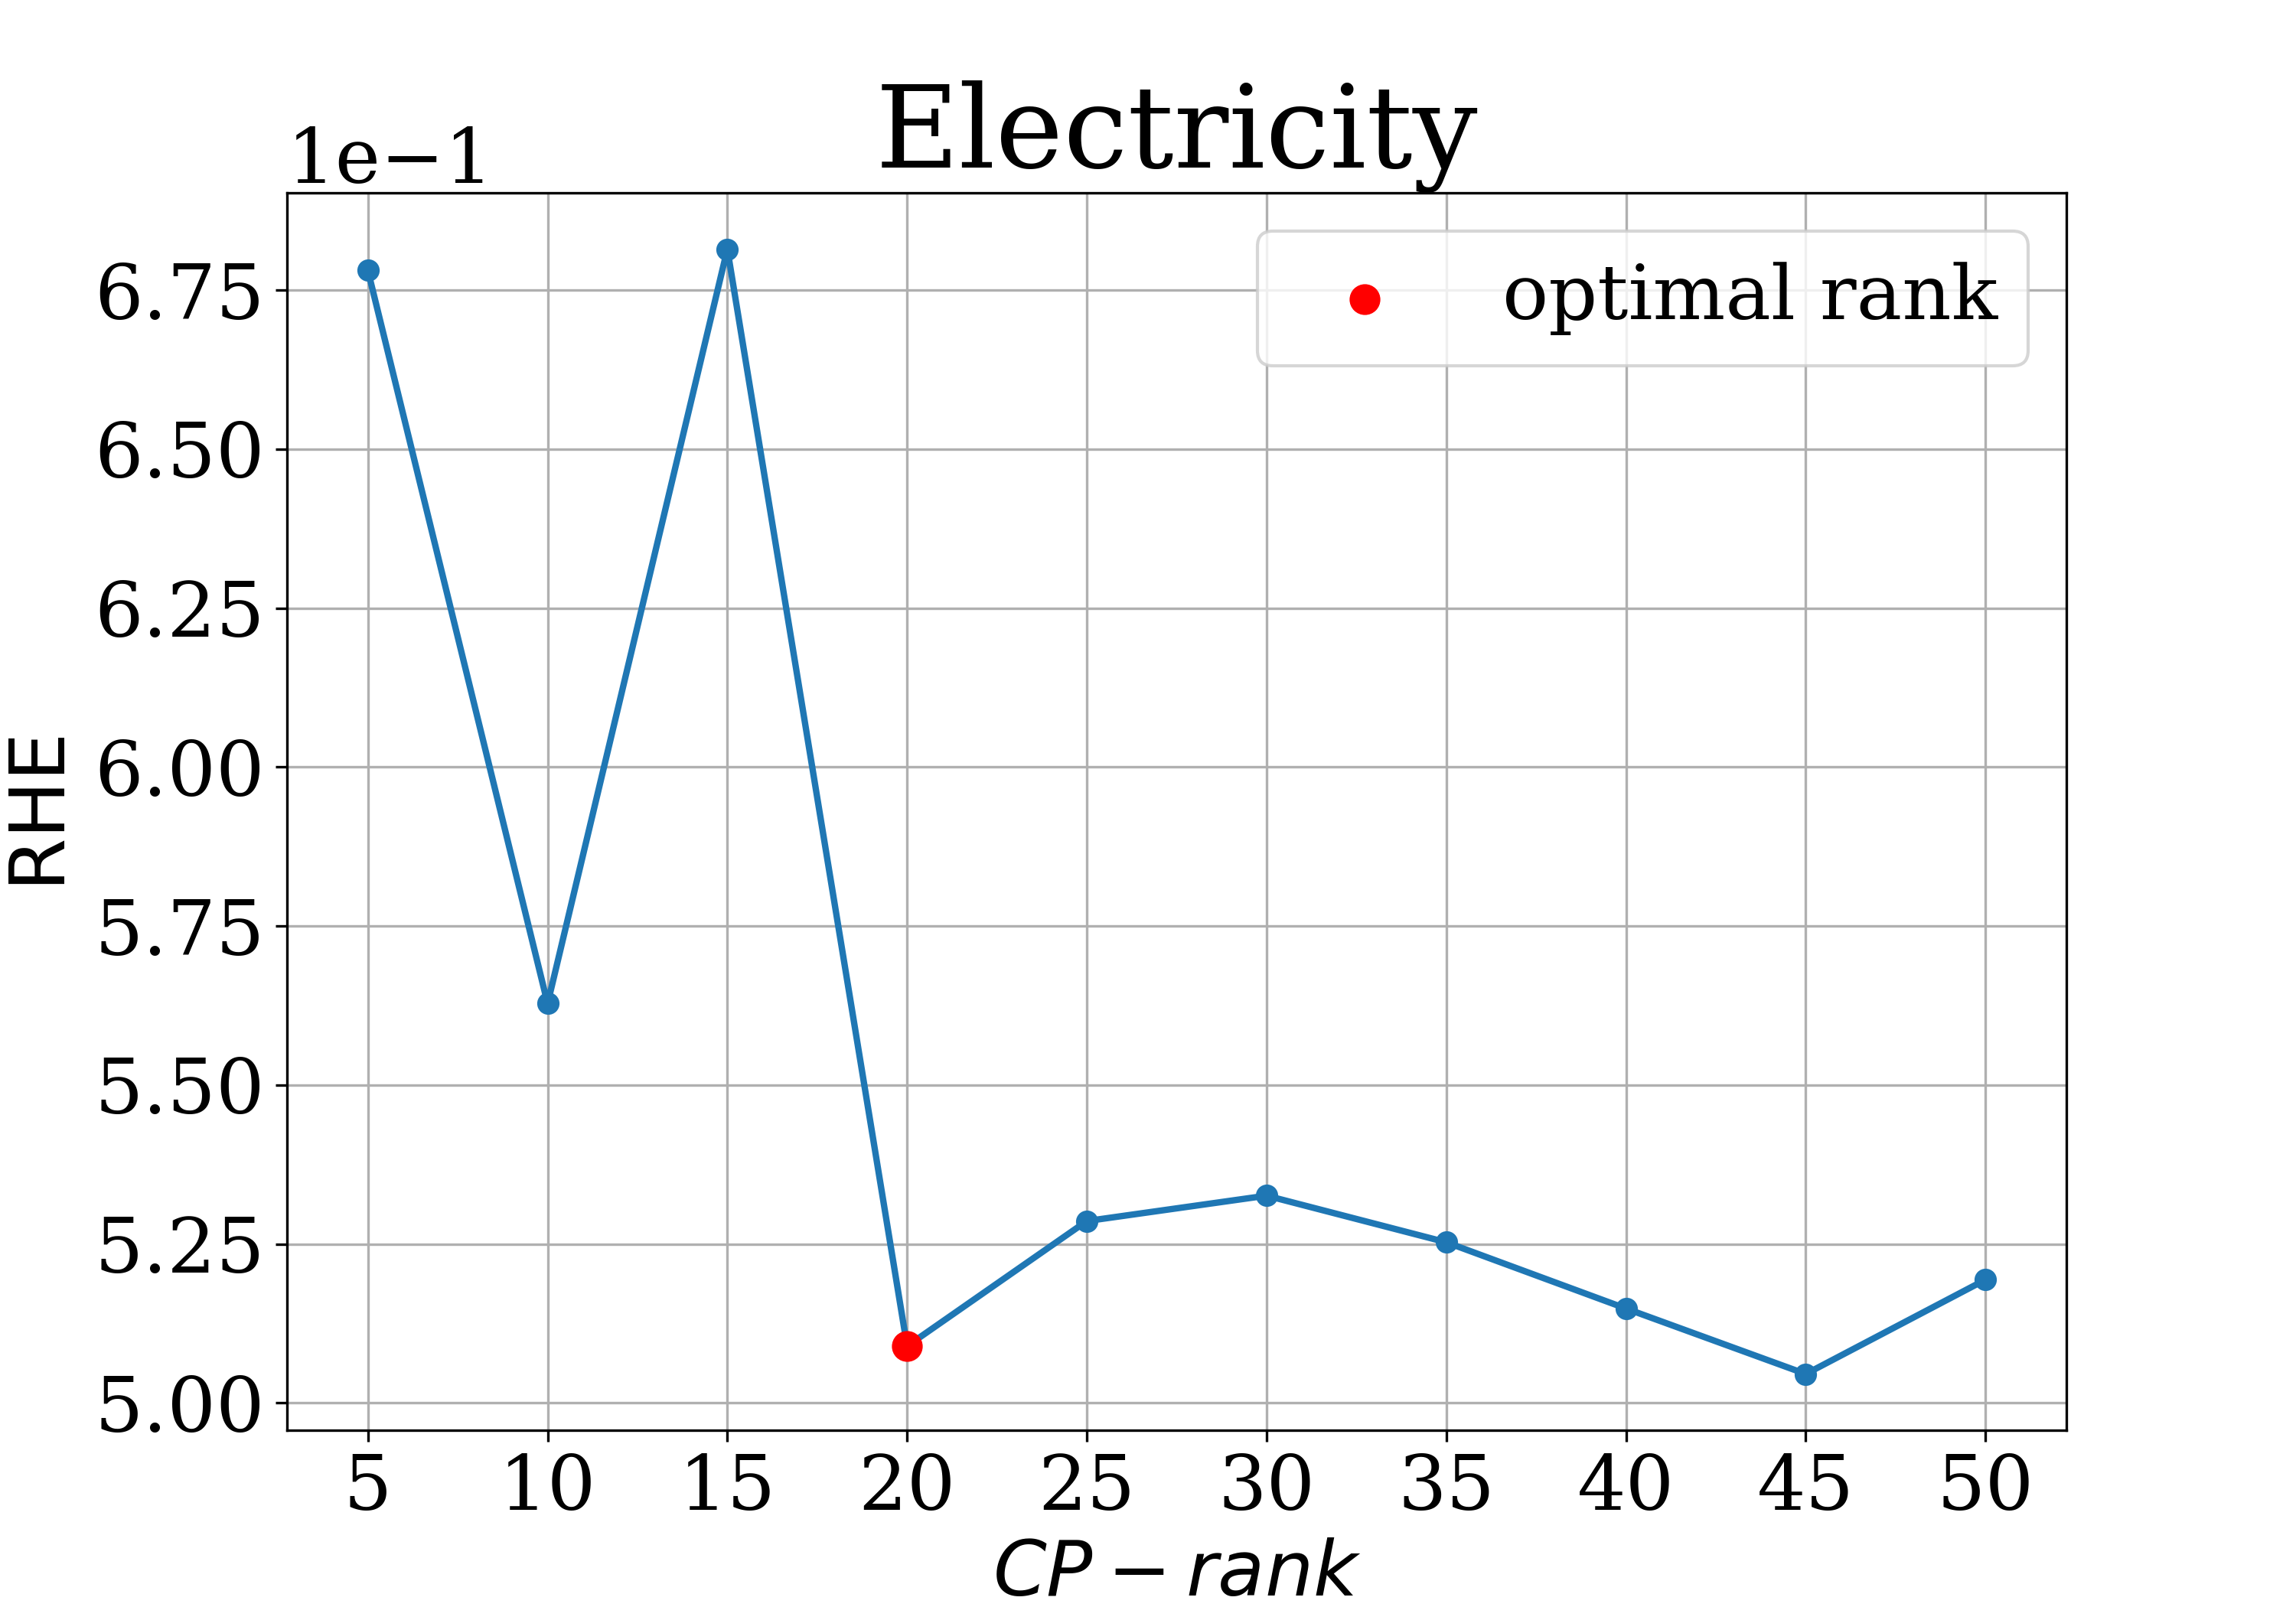
\includegraphics[width=0.48\textwidth, keepaspectratio]{RHE_mean_elec.png}
		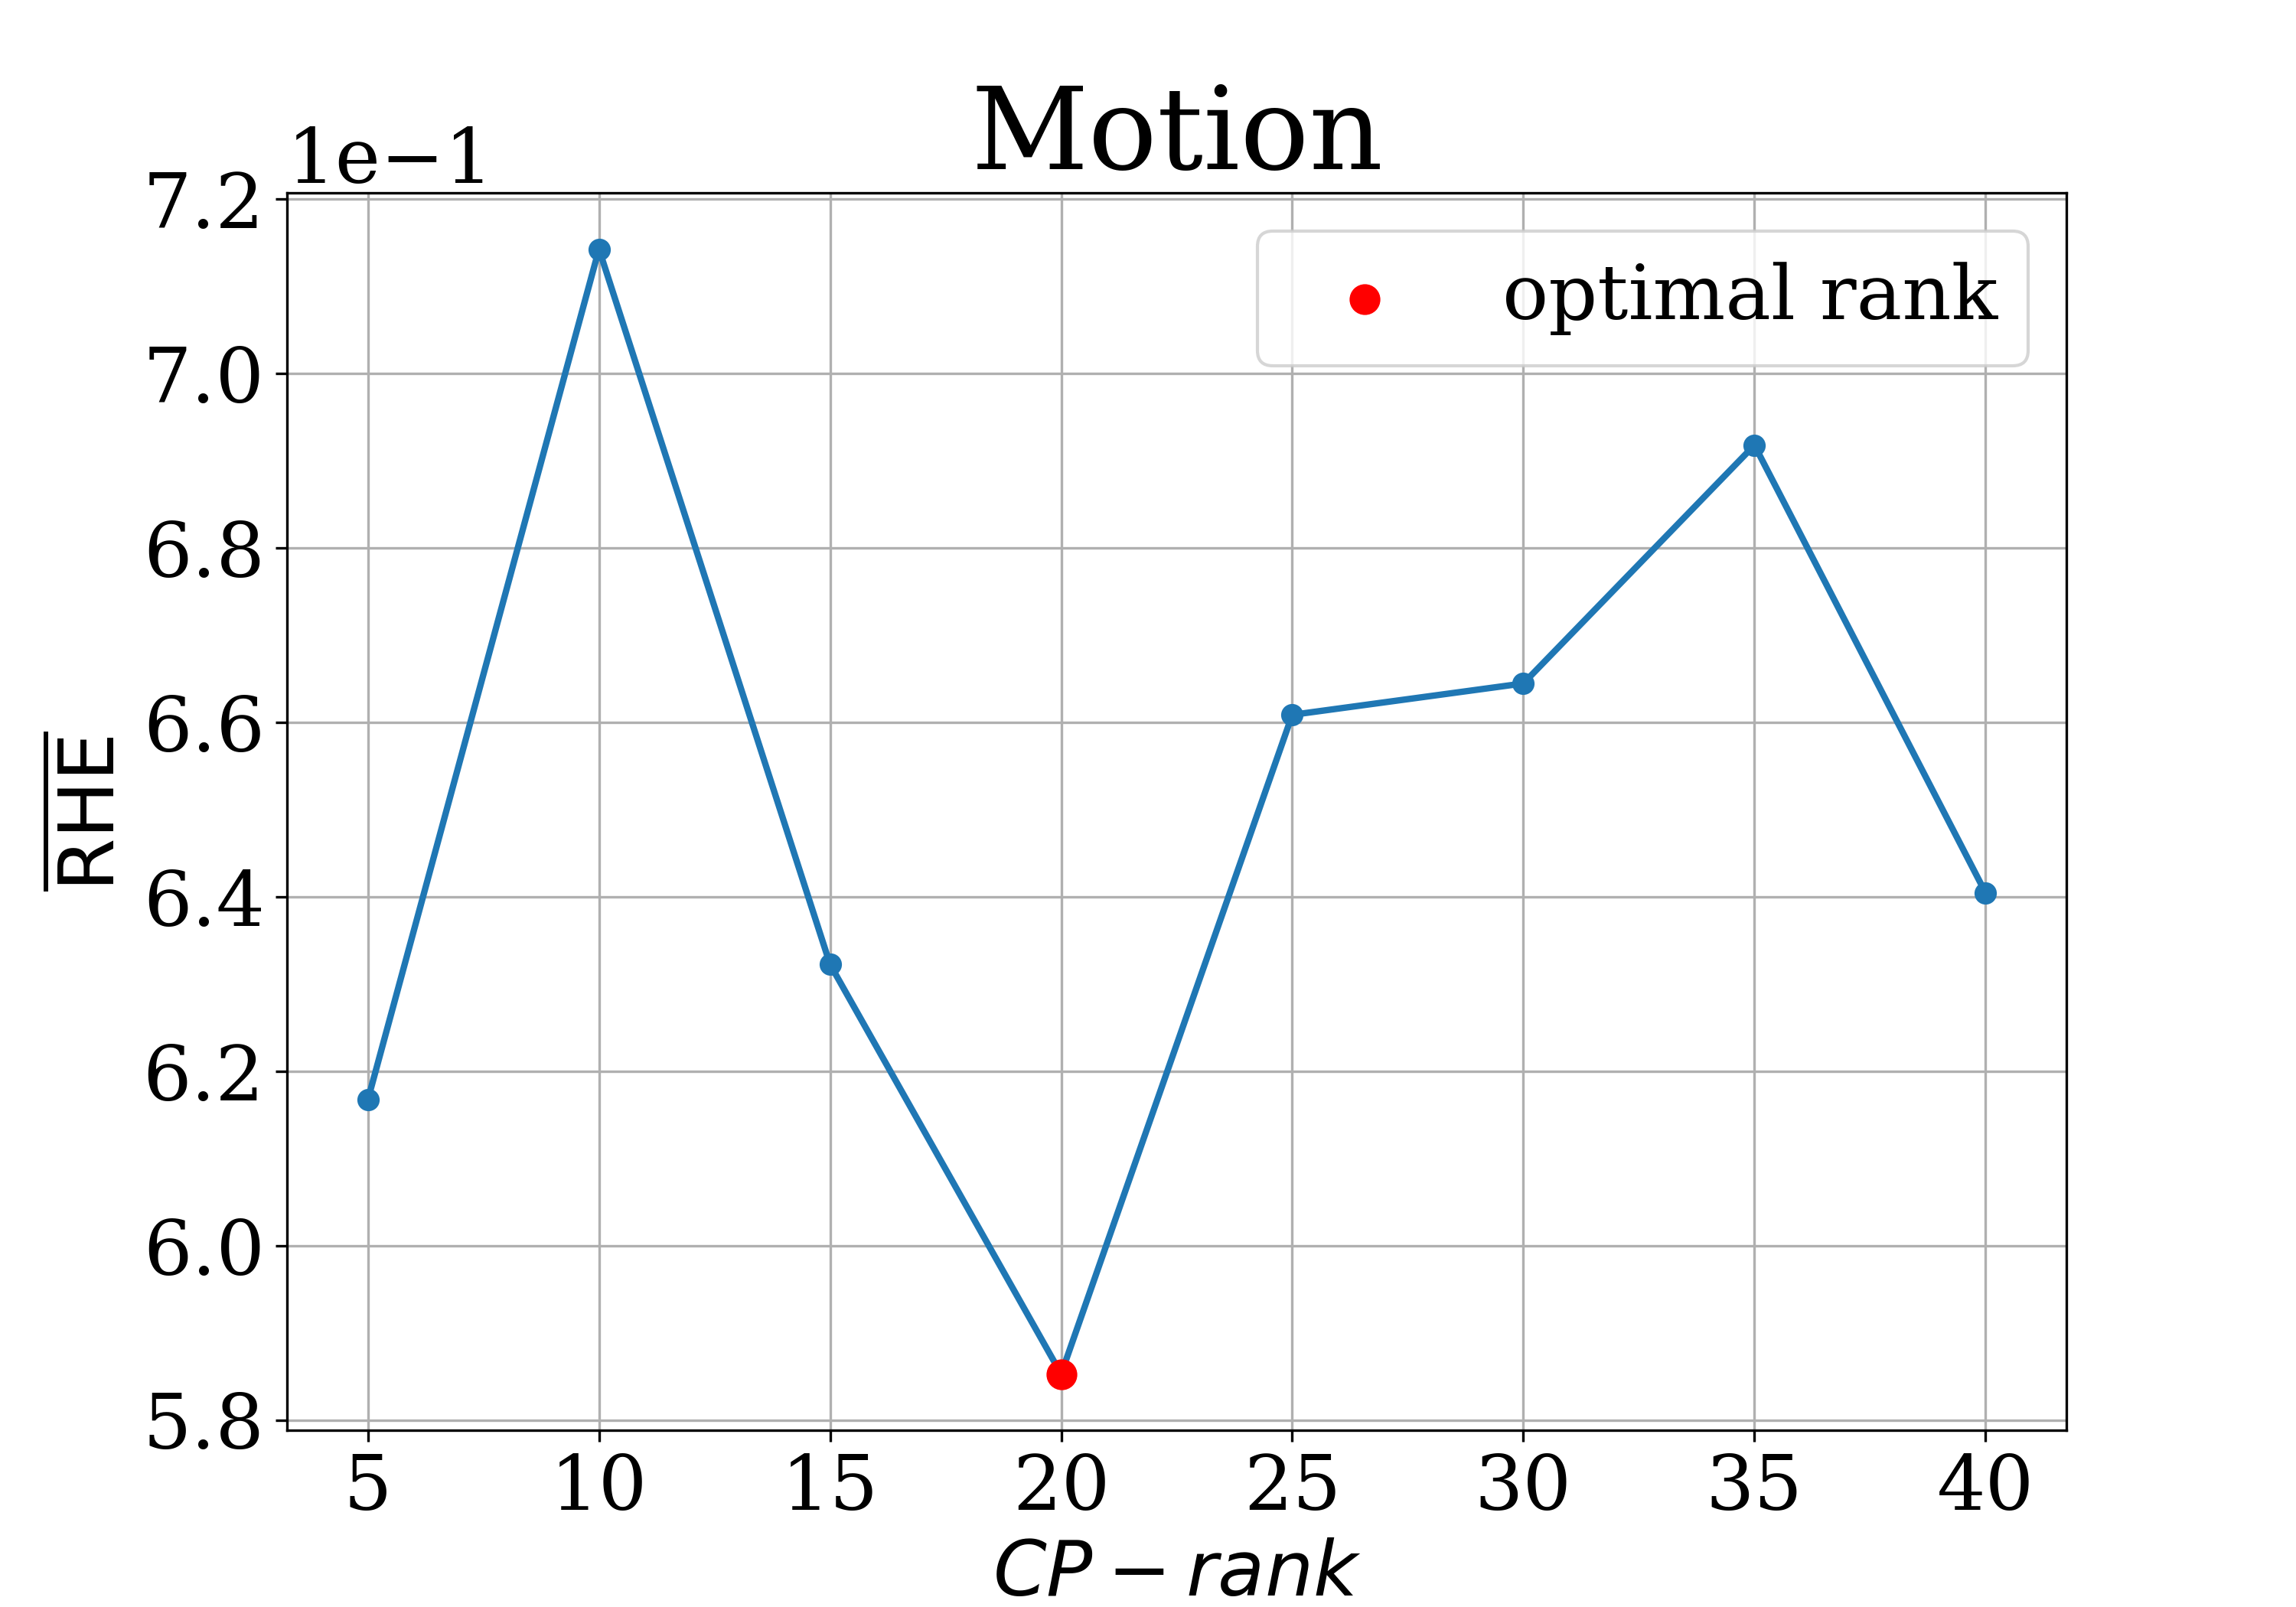
\includegraphics[width=0.48\textwidth, keepaspectratio]{RHE_mean_motion.png}
		\caption{Relationship between the $ \overline{\text{RHE}} $ metrics and the CPD rank. The left is for the electricity data, the right is for the inertial unit data. An optimal point is marked with red}\label{fig:decomp_rhe_rank}
	\end{figure}
	
	The decomposition on two components for the electricity consumption and its price is illustrated in the Fig. \ref{fig:electr_decomp_tssa}. The components are almost identical to the bias and scale factors. This is attributed to an effect of having the \emph{shared} phase space between the time series. Two-component decomposition for the accelerometer is shown in the Fig. \ref{fig:accel_decomp_tssa} and for the gyroscope in the Fig. \ref{fig:gyro_decomp_tssa}. The same effect is seen for the second components here.
	
	\begin{figure}[h]
		\centering
		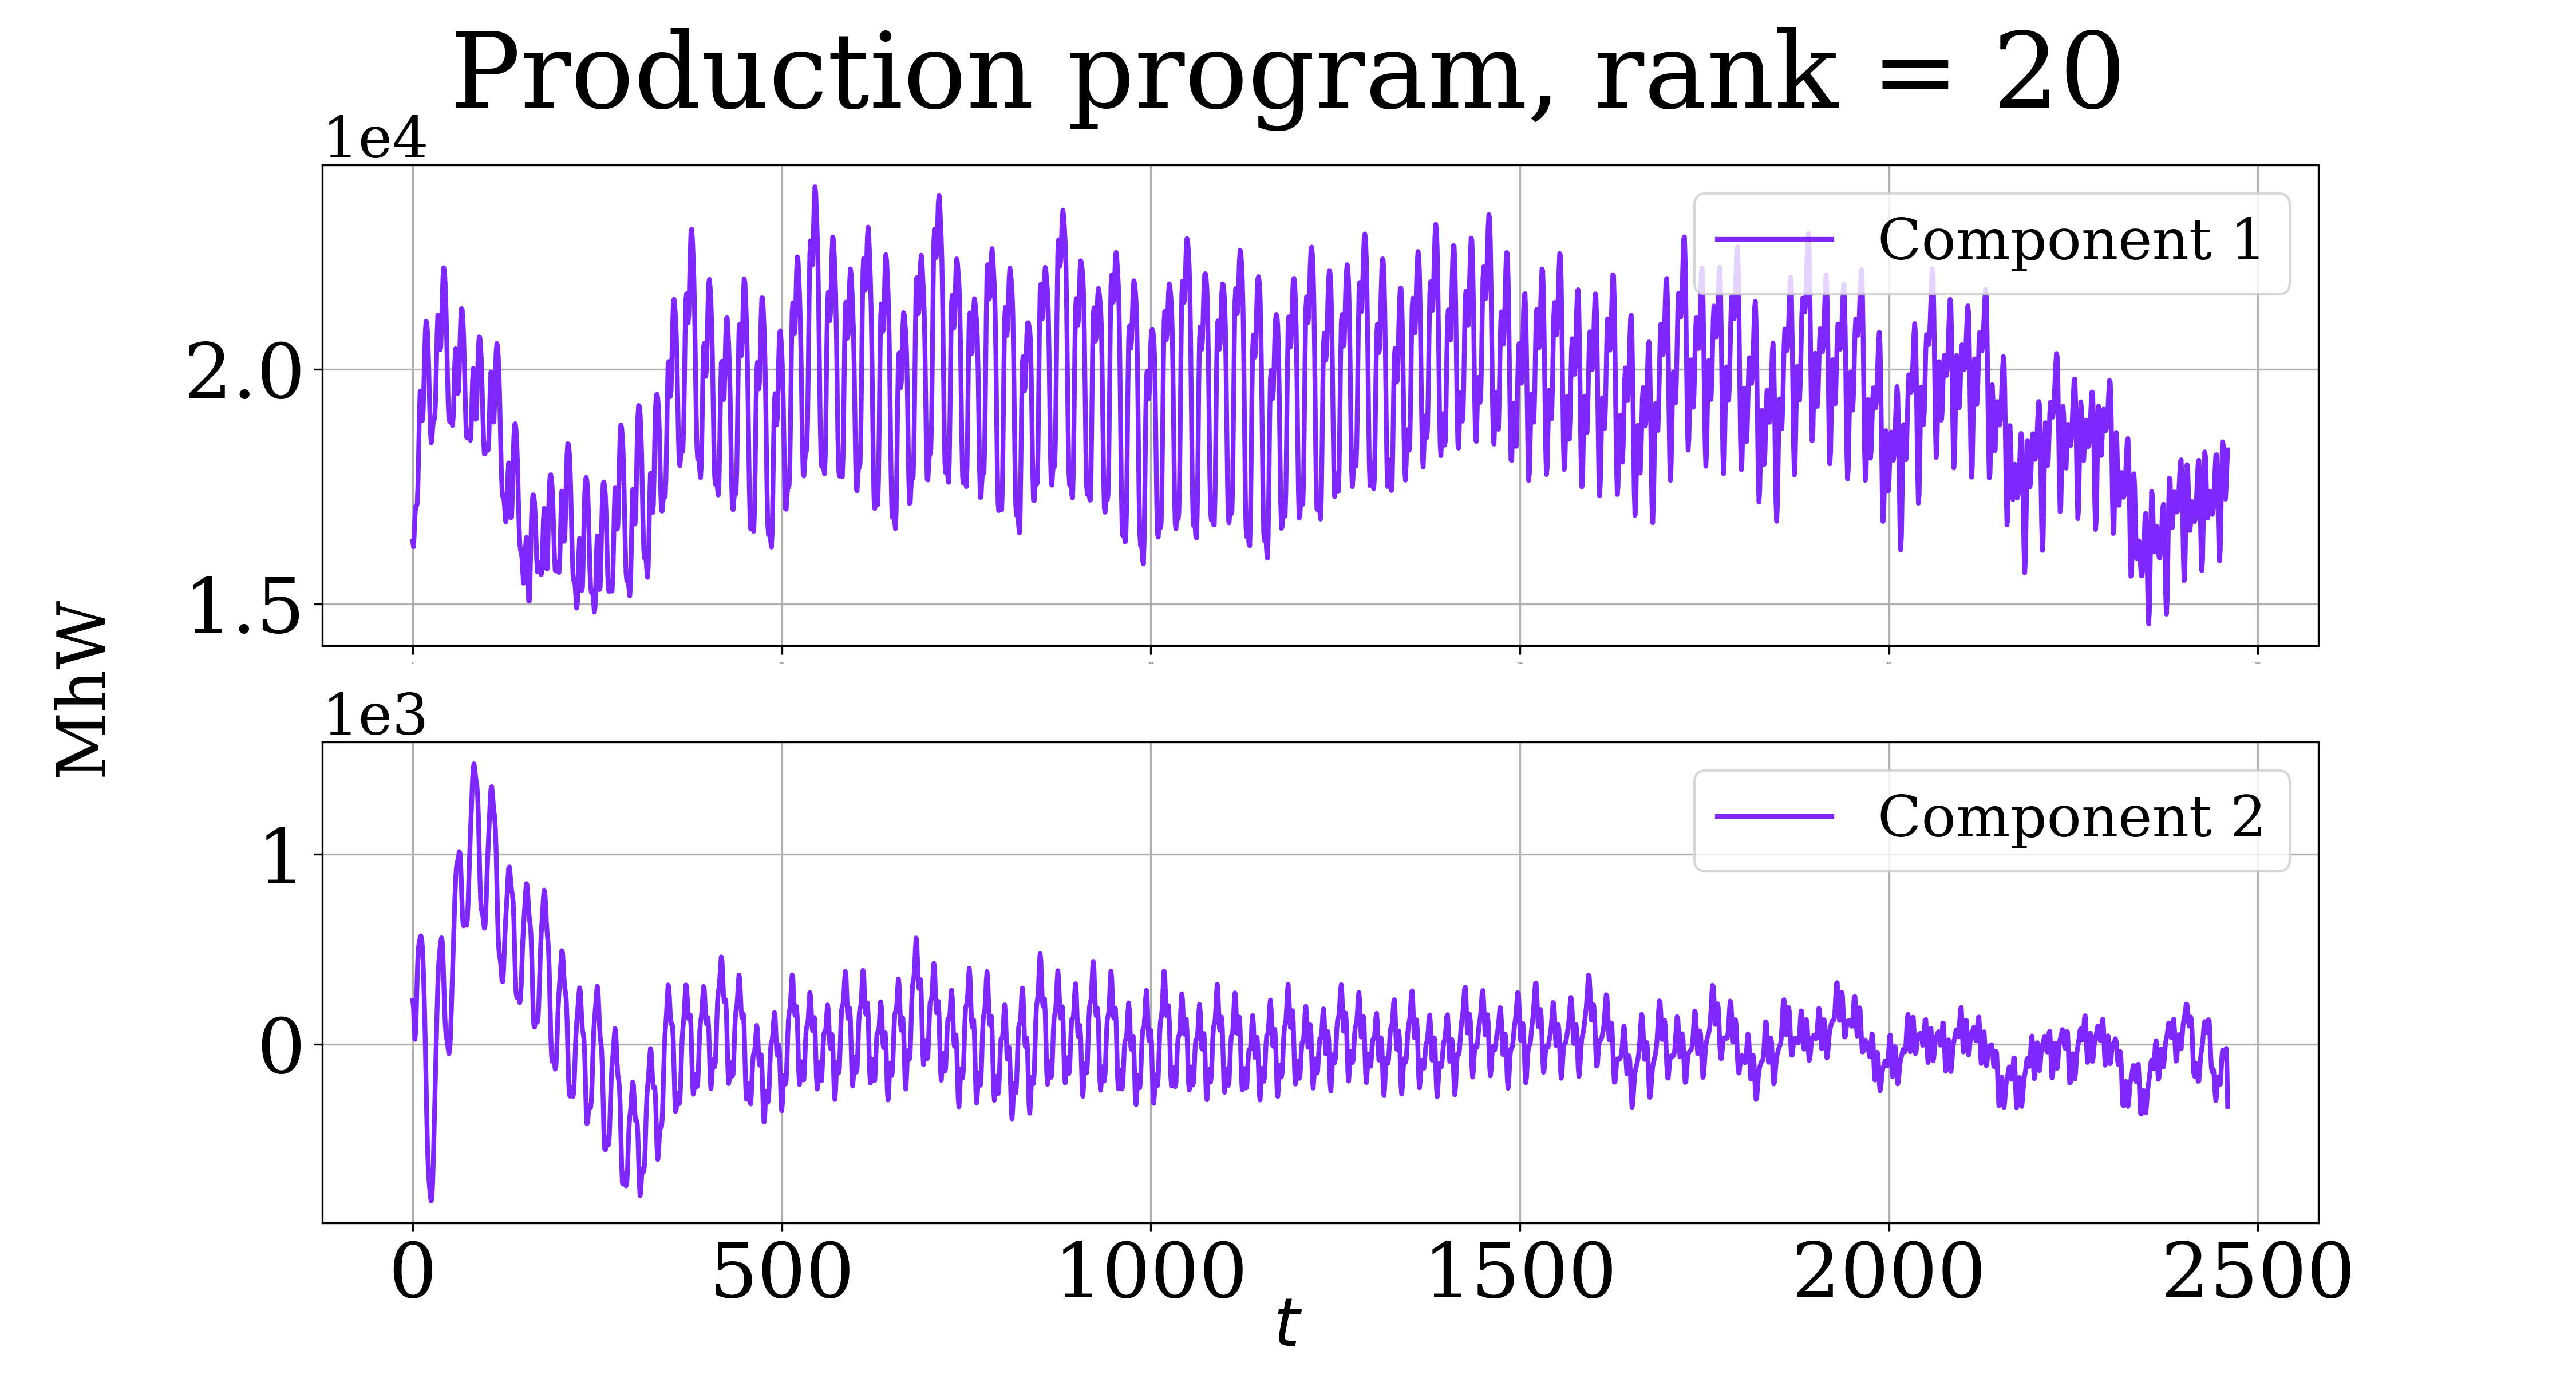
\includegraphics[width=0.48\textwidth, keepaspectratio]{Production program_decomp.png}
		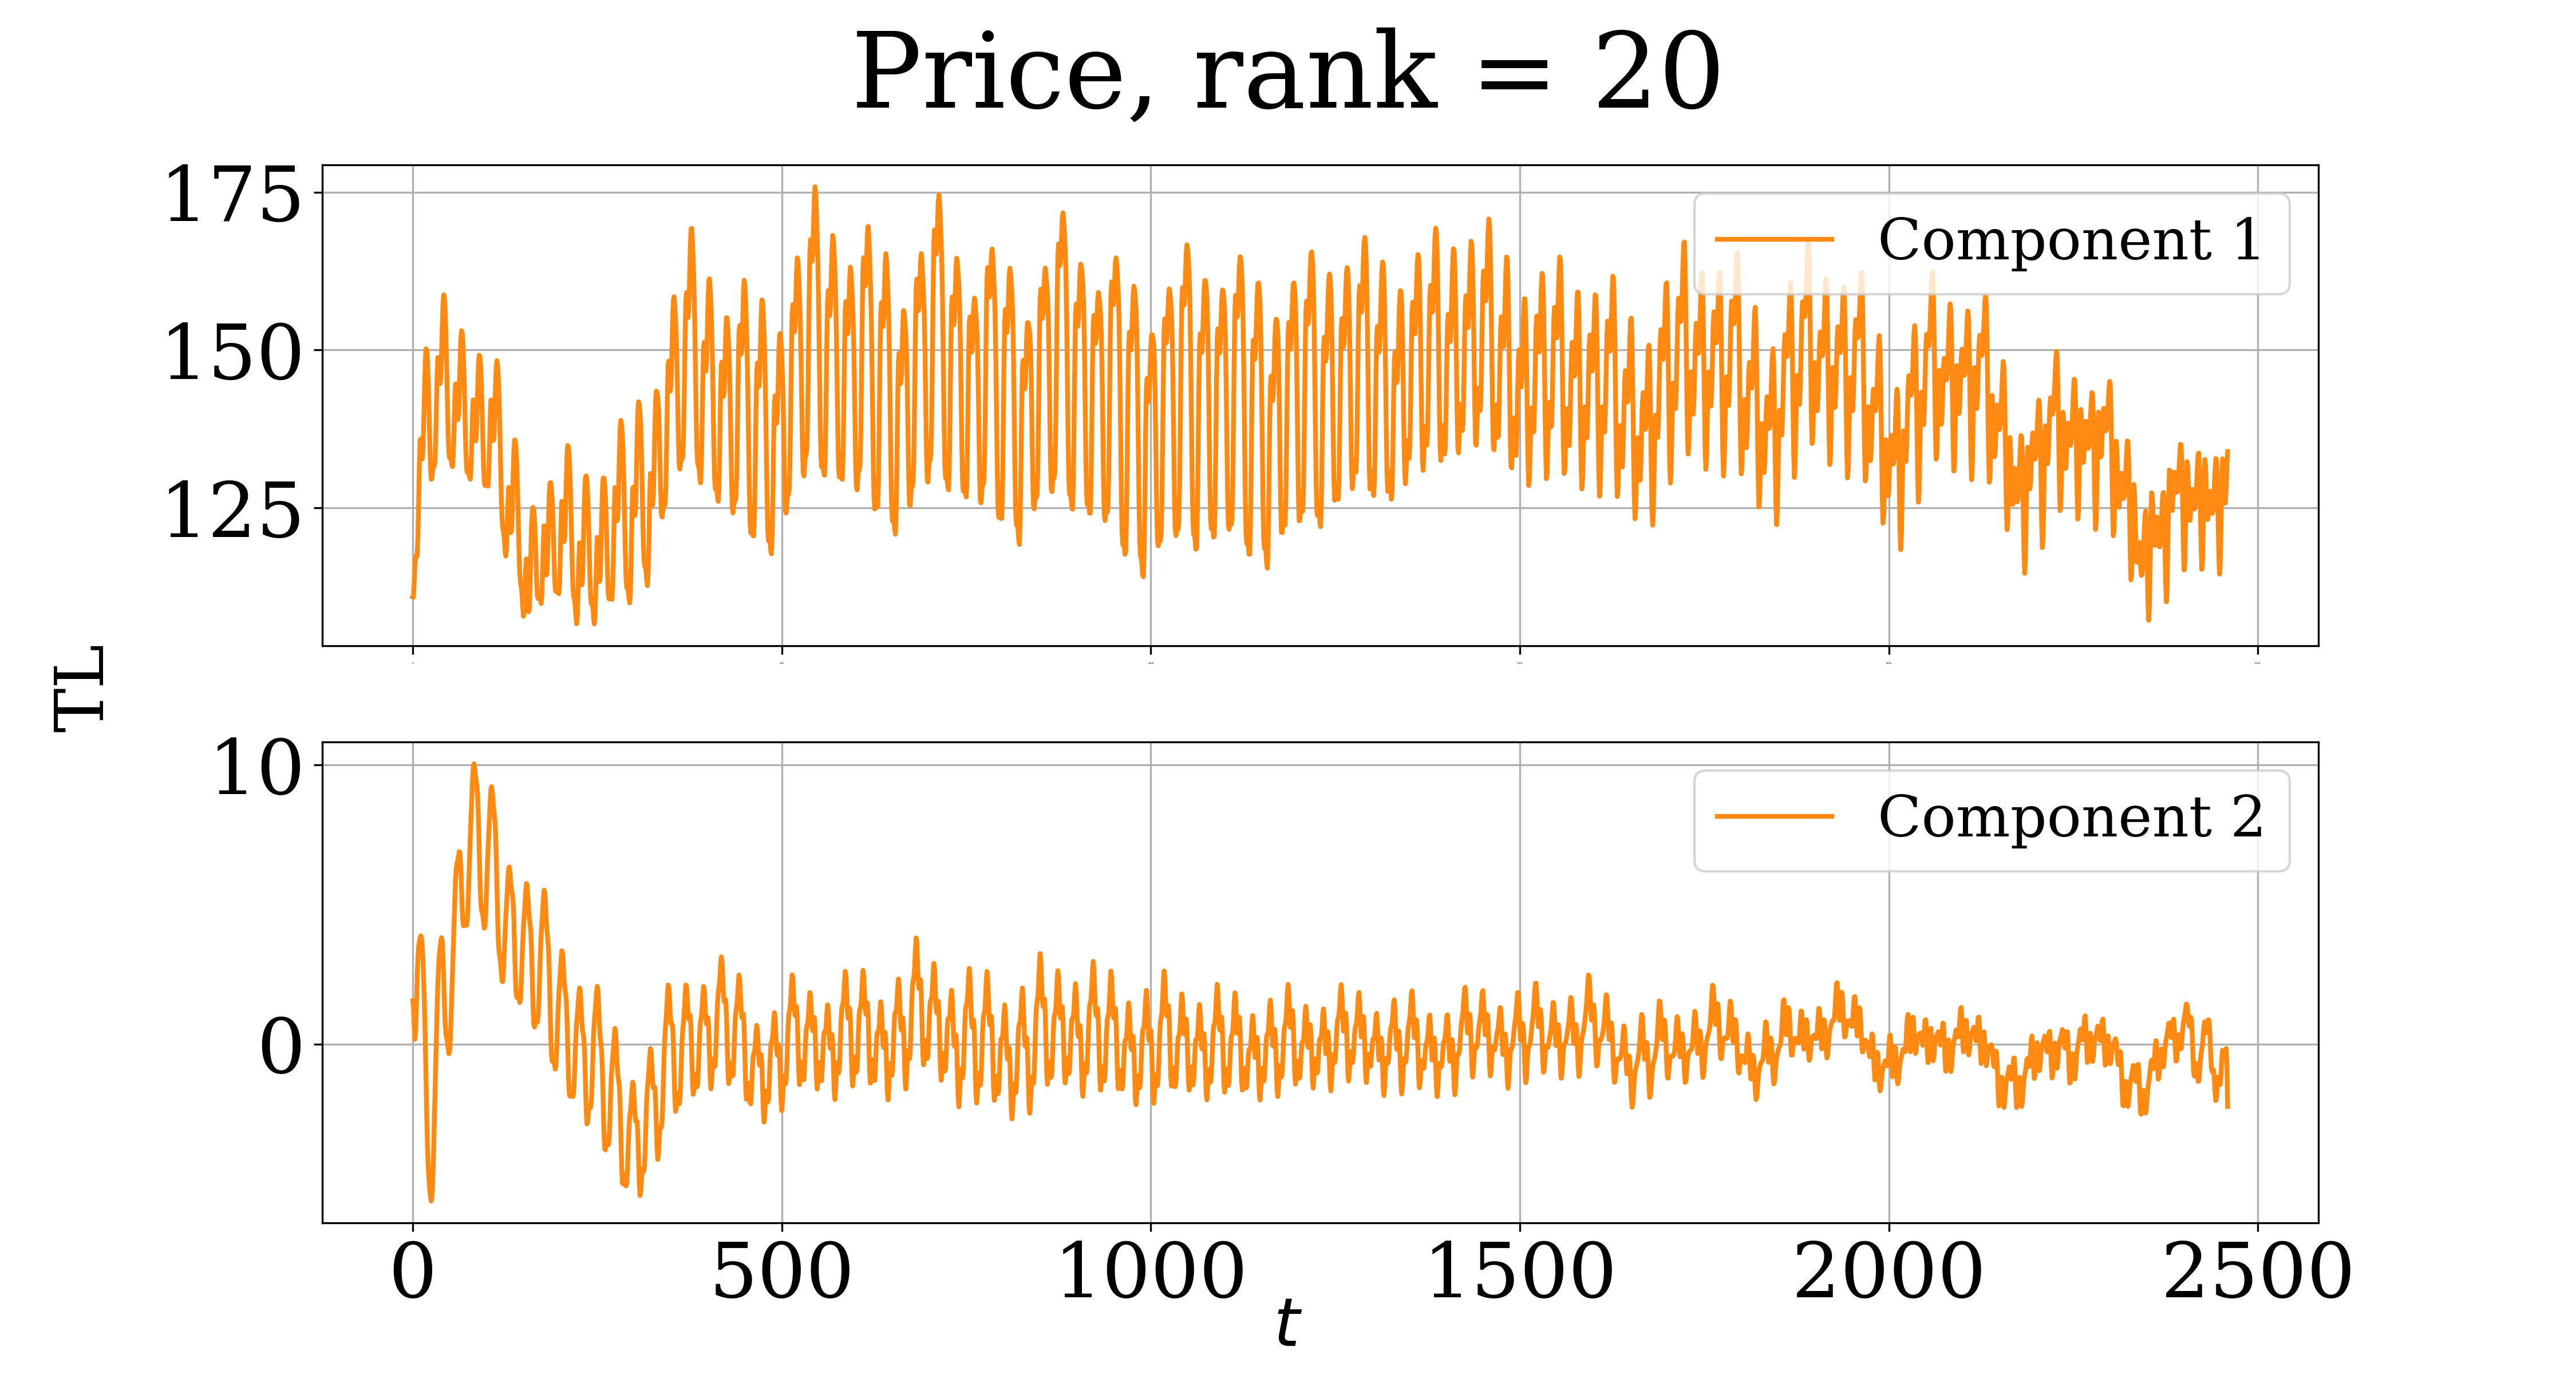
\includegraphics[width=0.48\textwidth, keepaspectratio]{Price_decomp.png}
		\caption{tSSA decomposition for the electricity data. CPD rank $ = 20 $}\label{fig:electr_decomp_tssa}
	\end{figure}
	
	\begin{figure}[h]
		\centering
		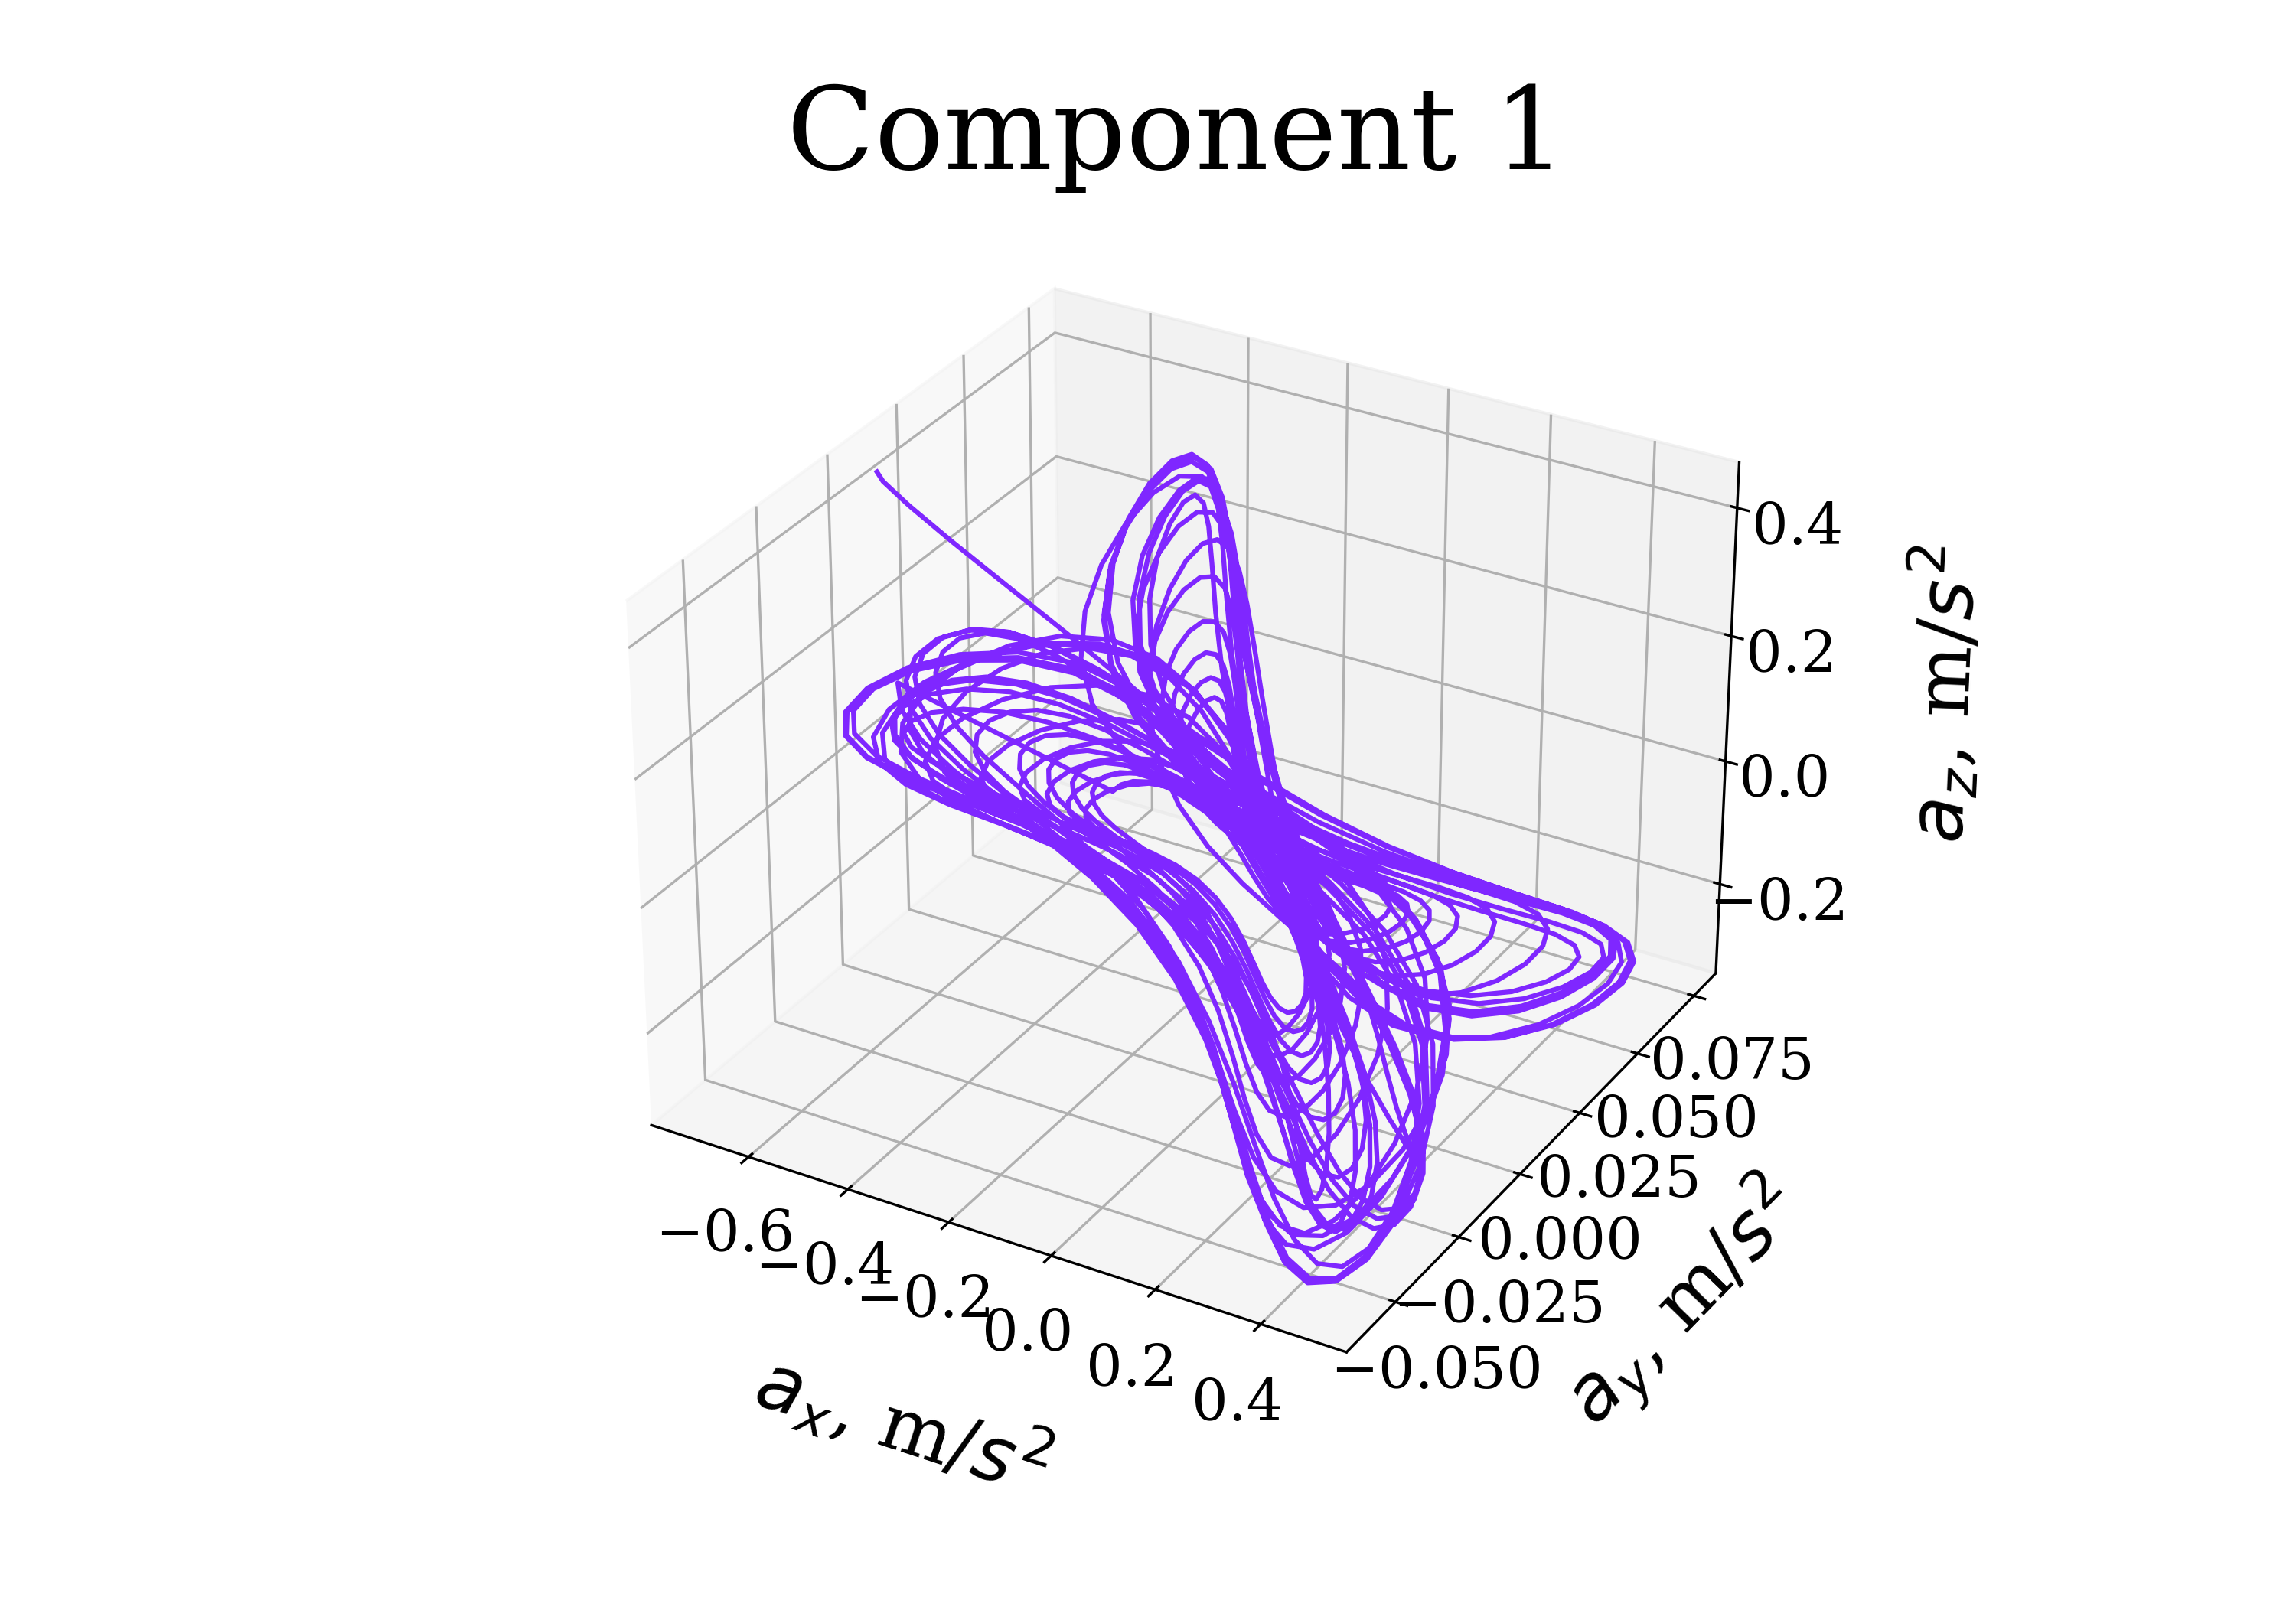
\includegraphics[width=0.48\textwidth, 	keepaspectratio]{acceler_1.png}
		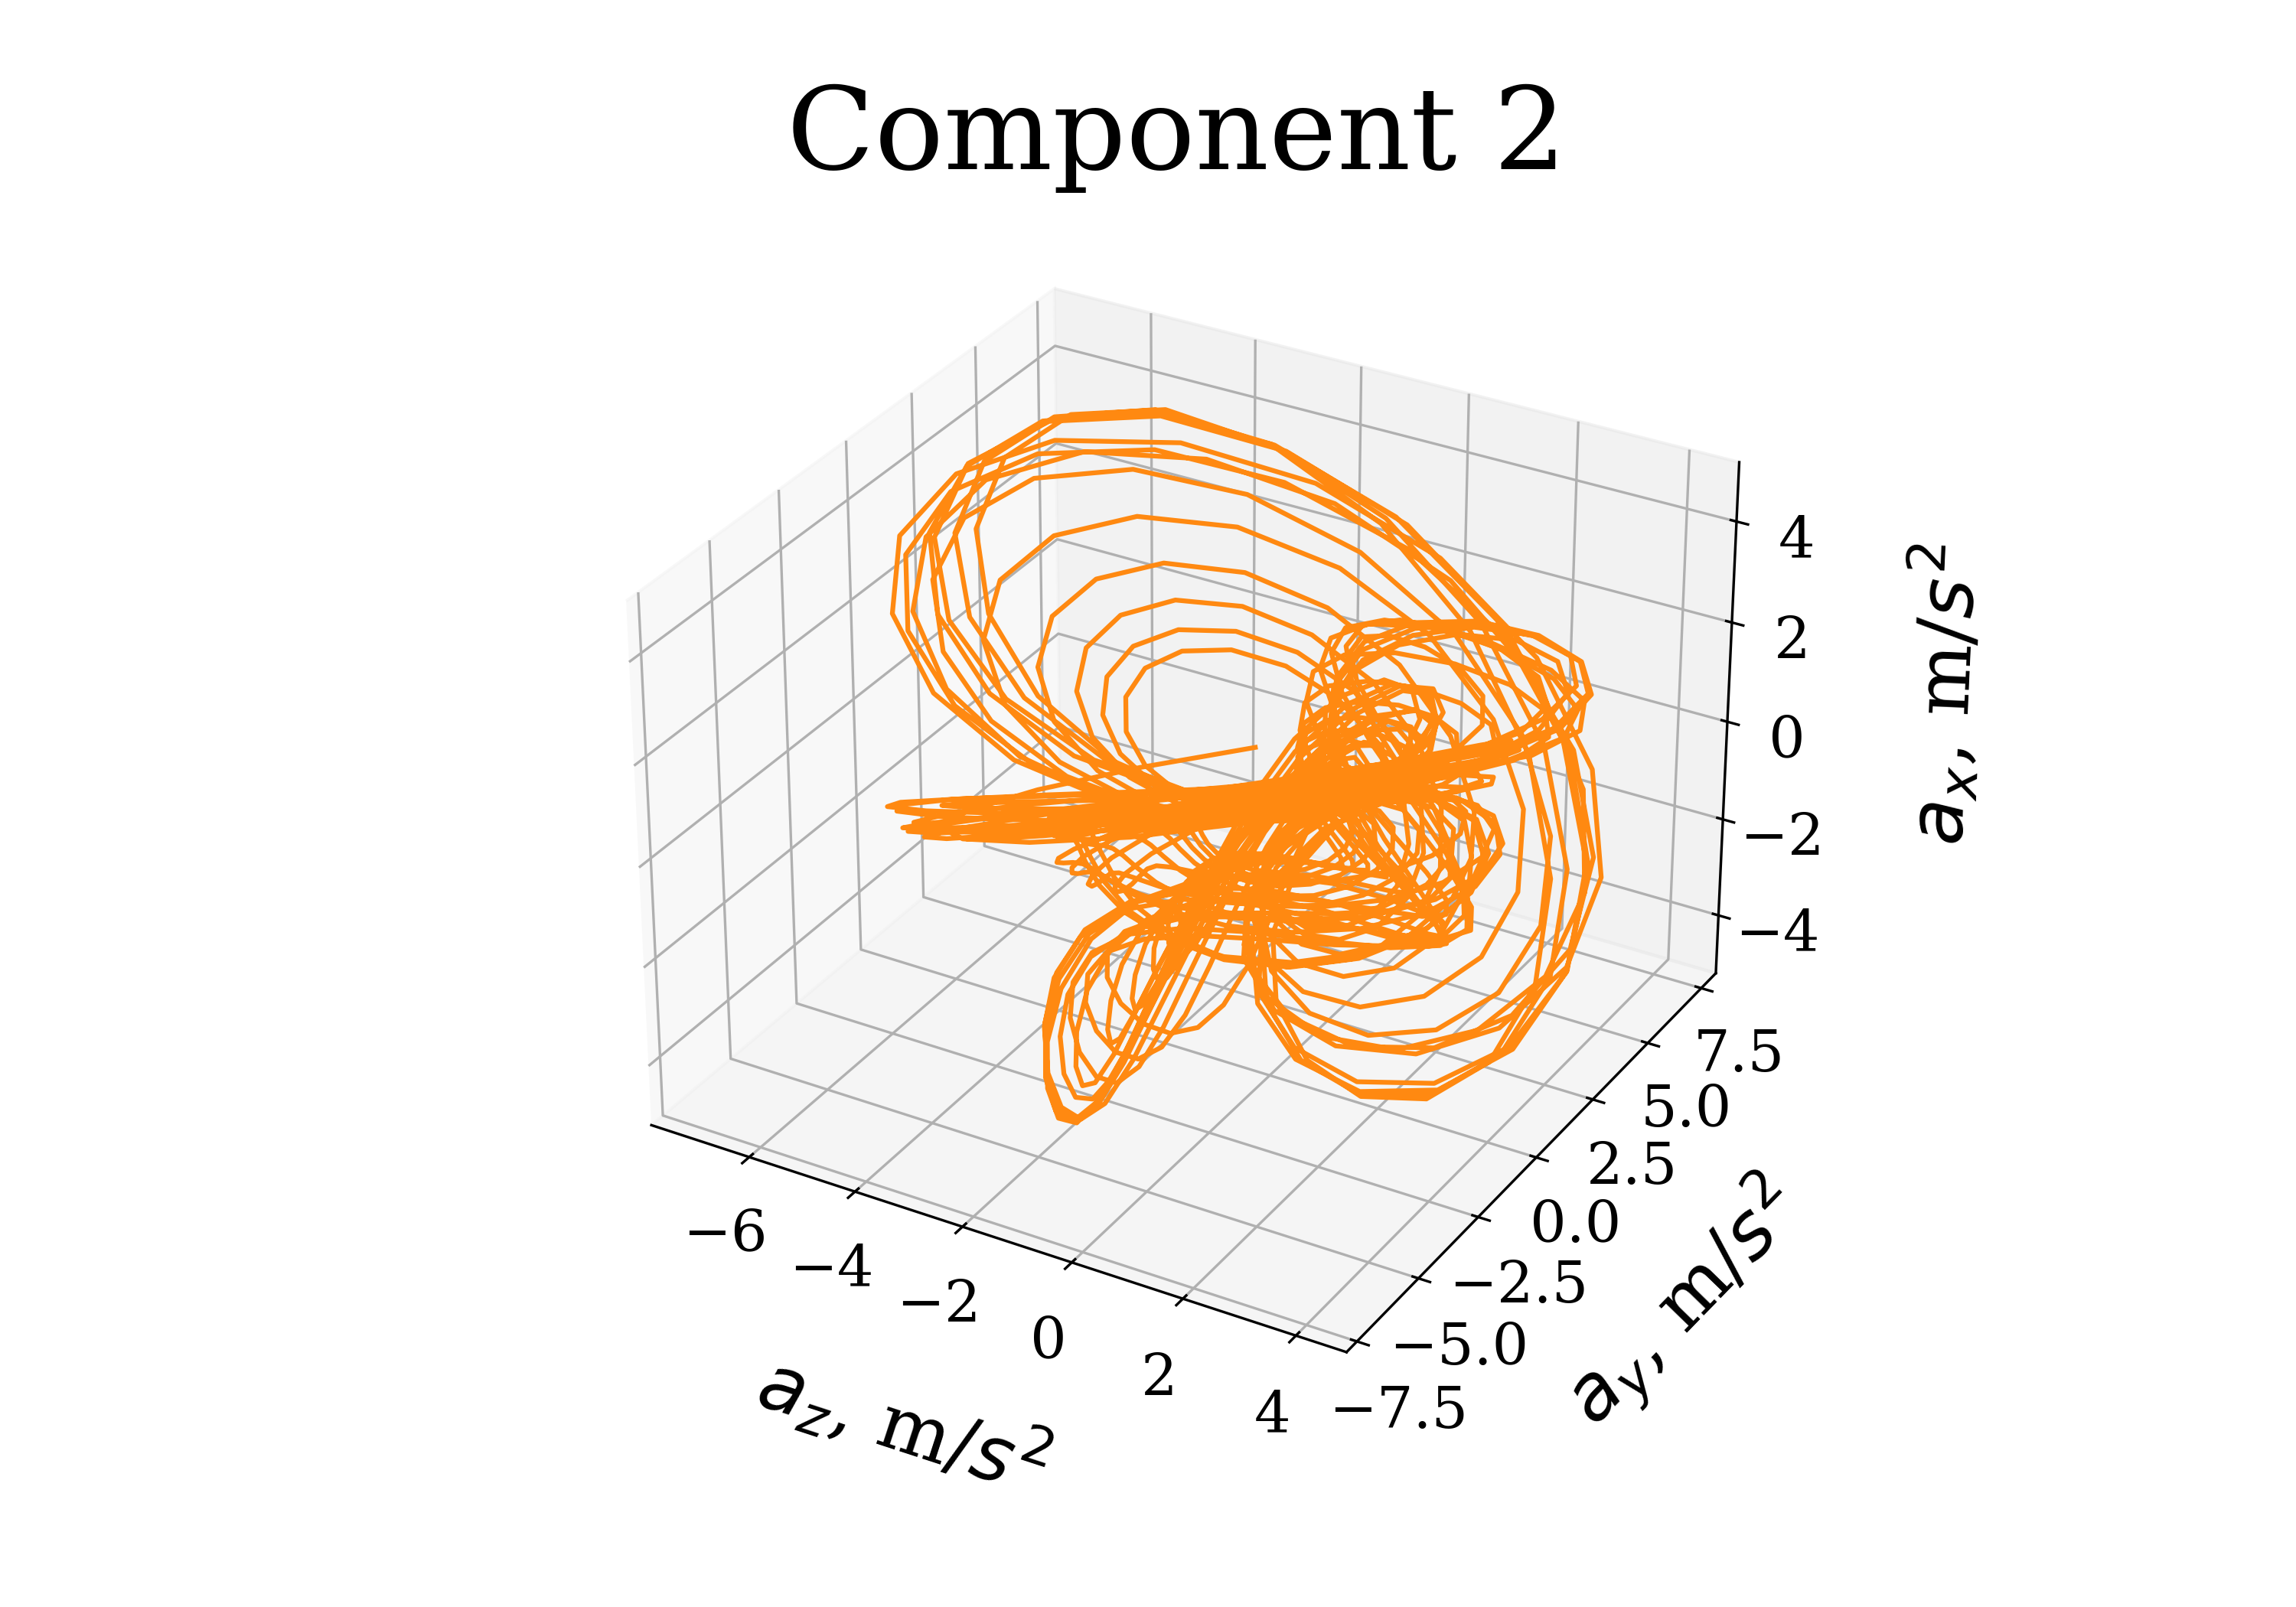
\includegraphics[width=0.48\textwidth, keepaspectratio]{acceler_2.png}
		\caption{tSSA decomposition for the accelerometer data. CPD rank $ = 10 $}\label{fig:accel_decomp_tssa}
	\end{figure}
	
	\begin{figure}[h]
		\centering
		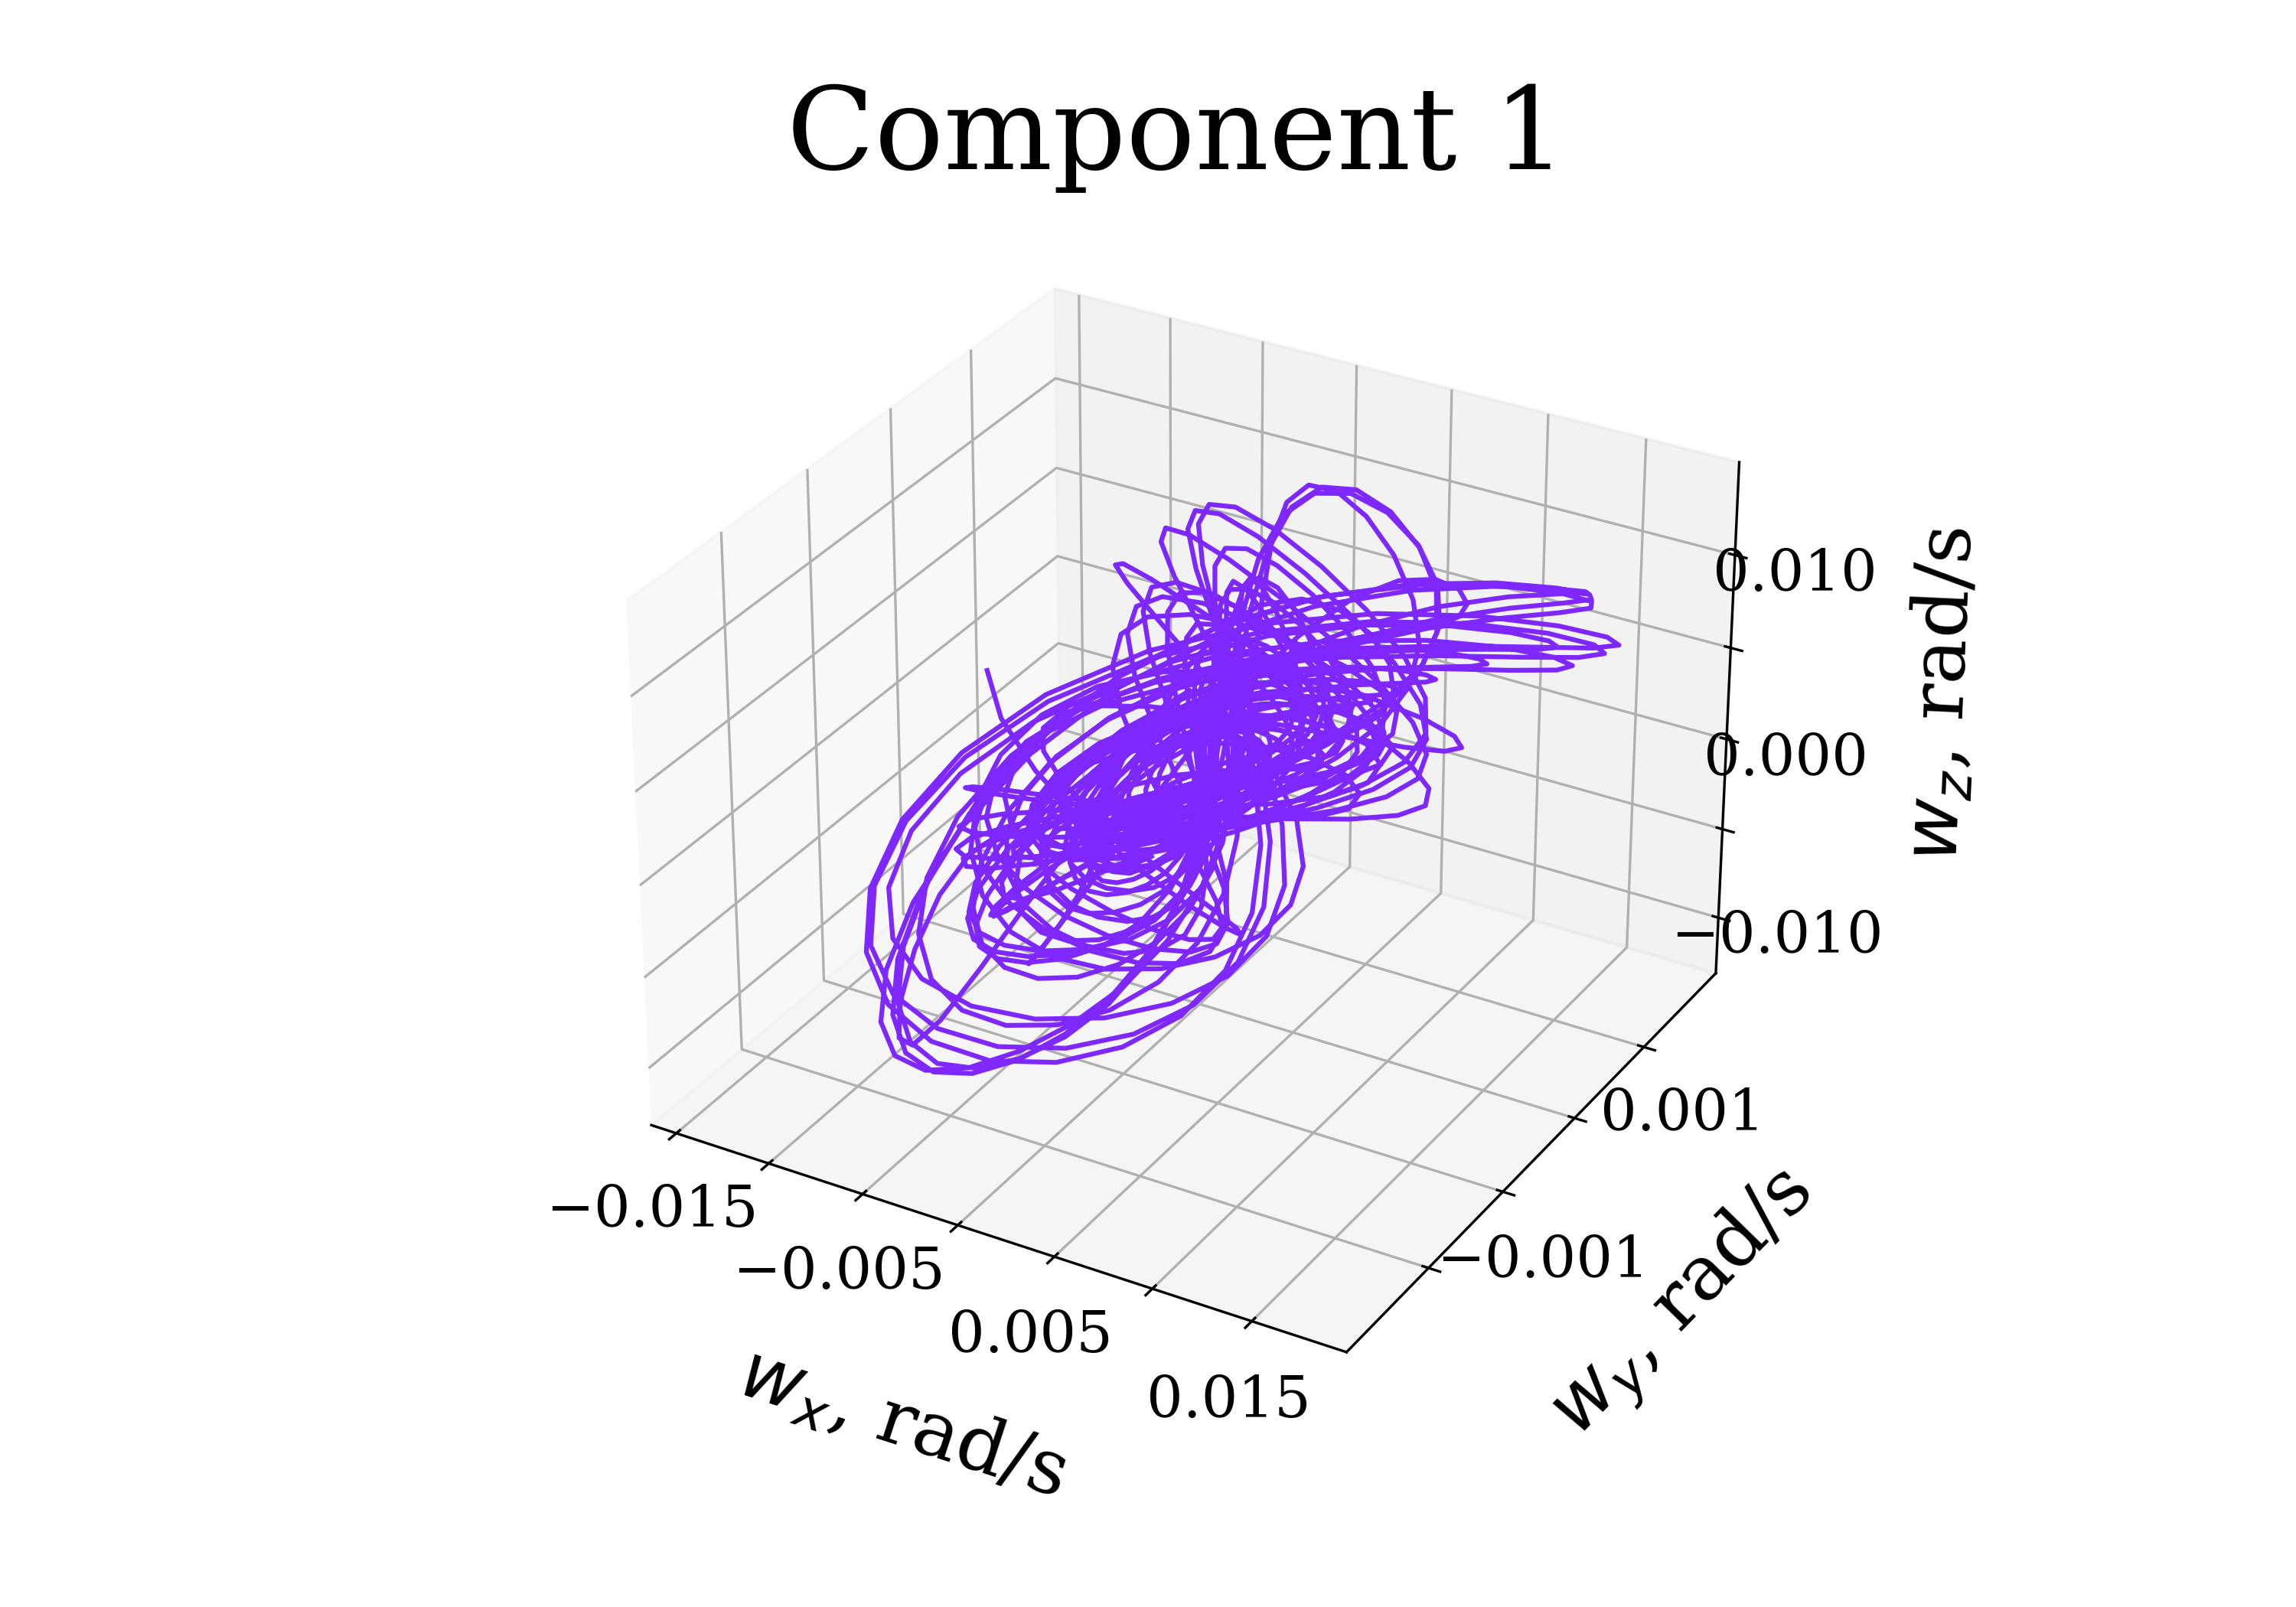
\includegraphics[width=0.48\textwidth, 	keepaspectratio]{gyro_1.png}
		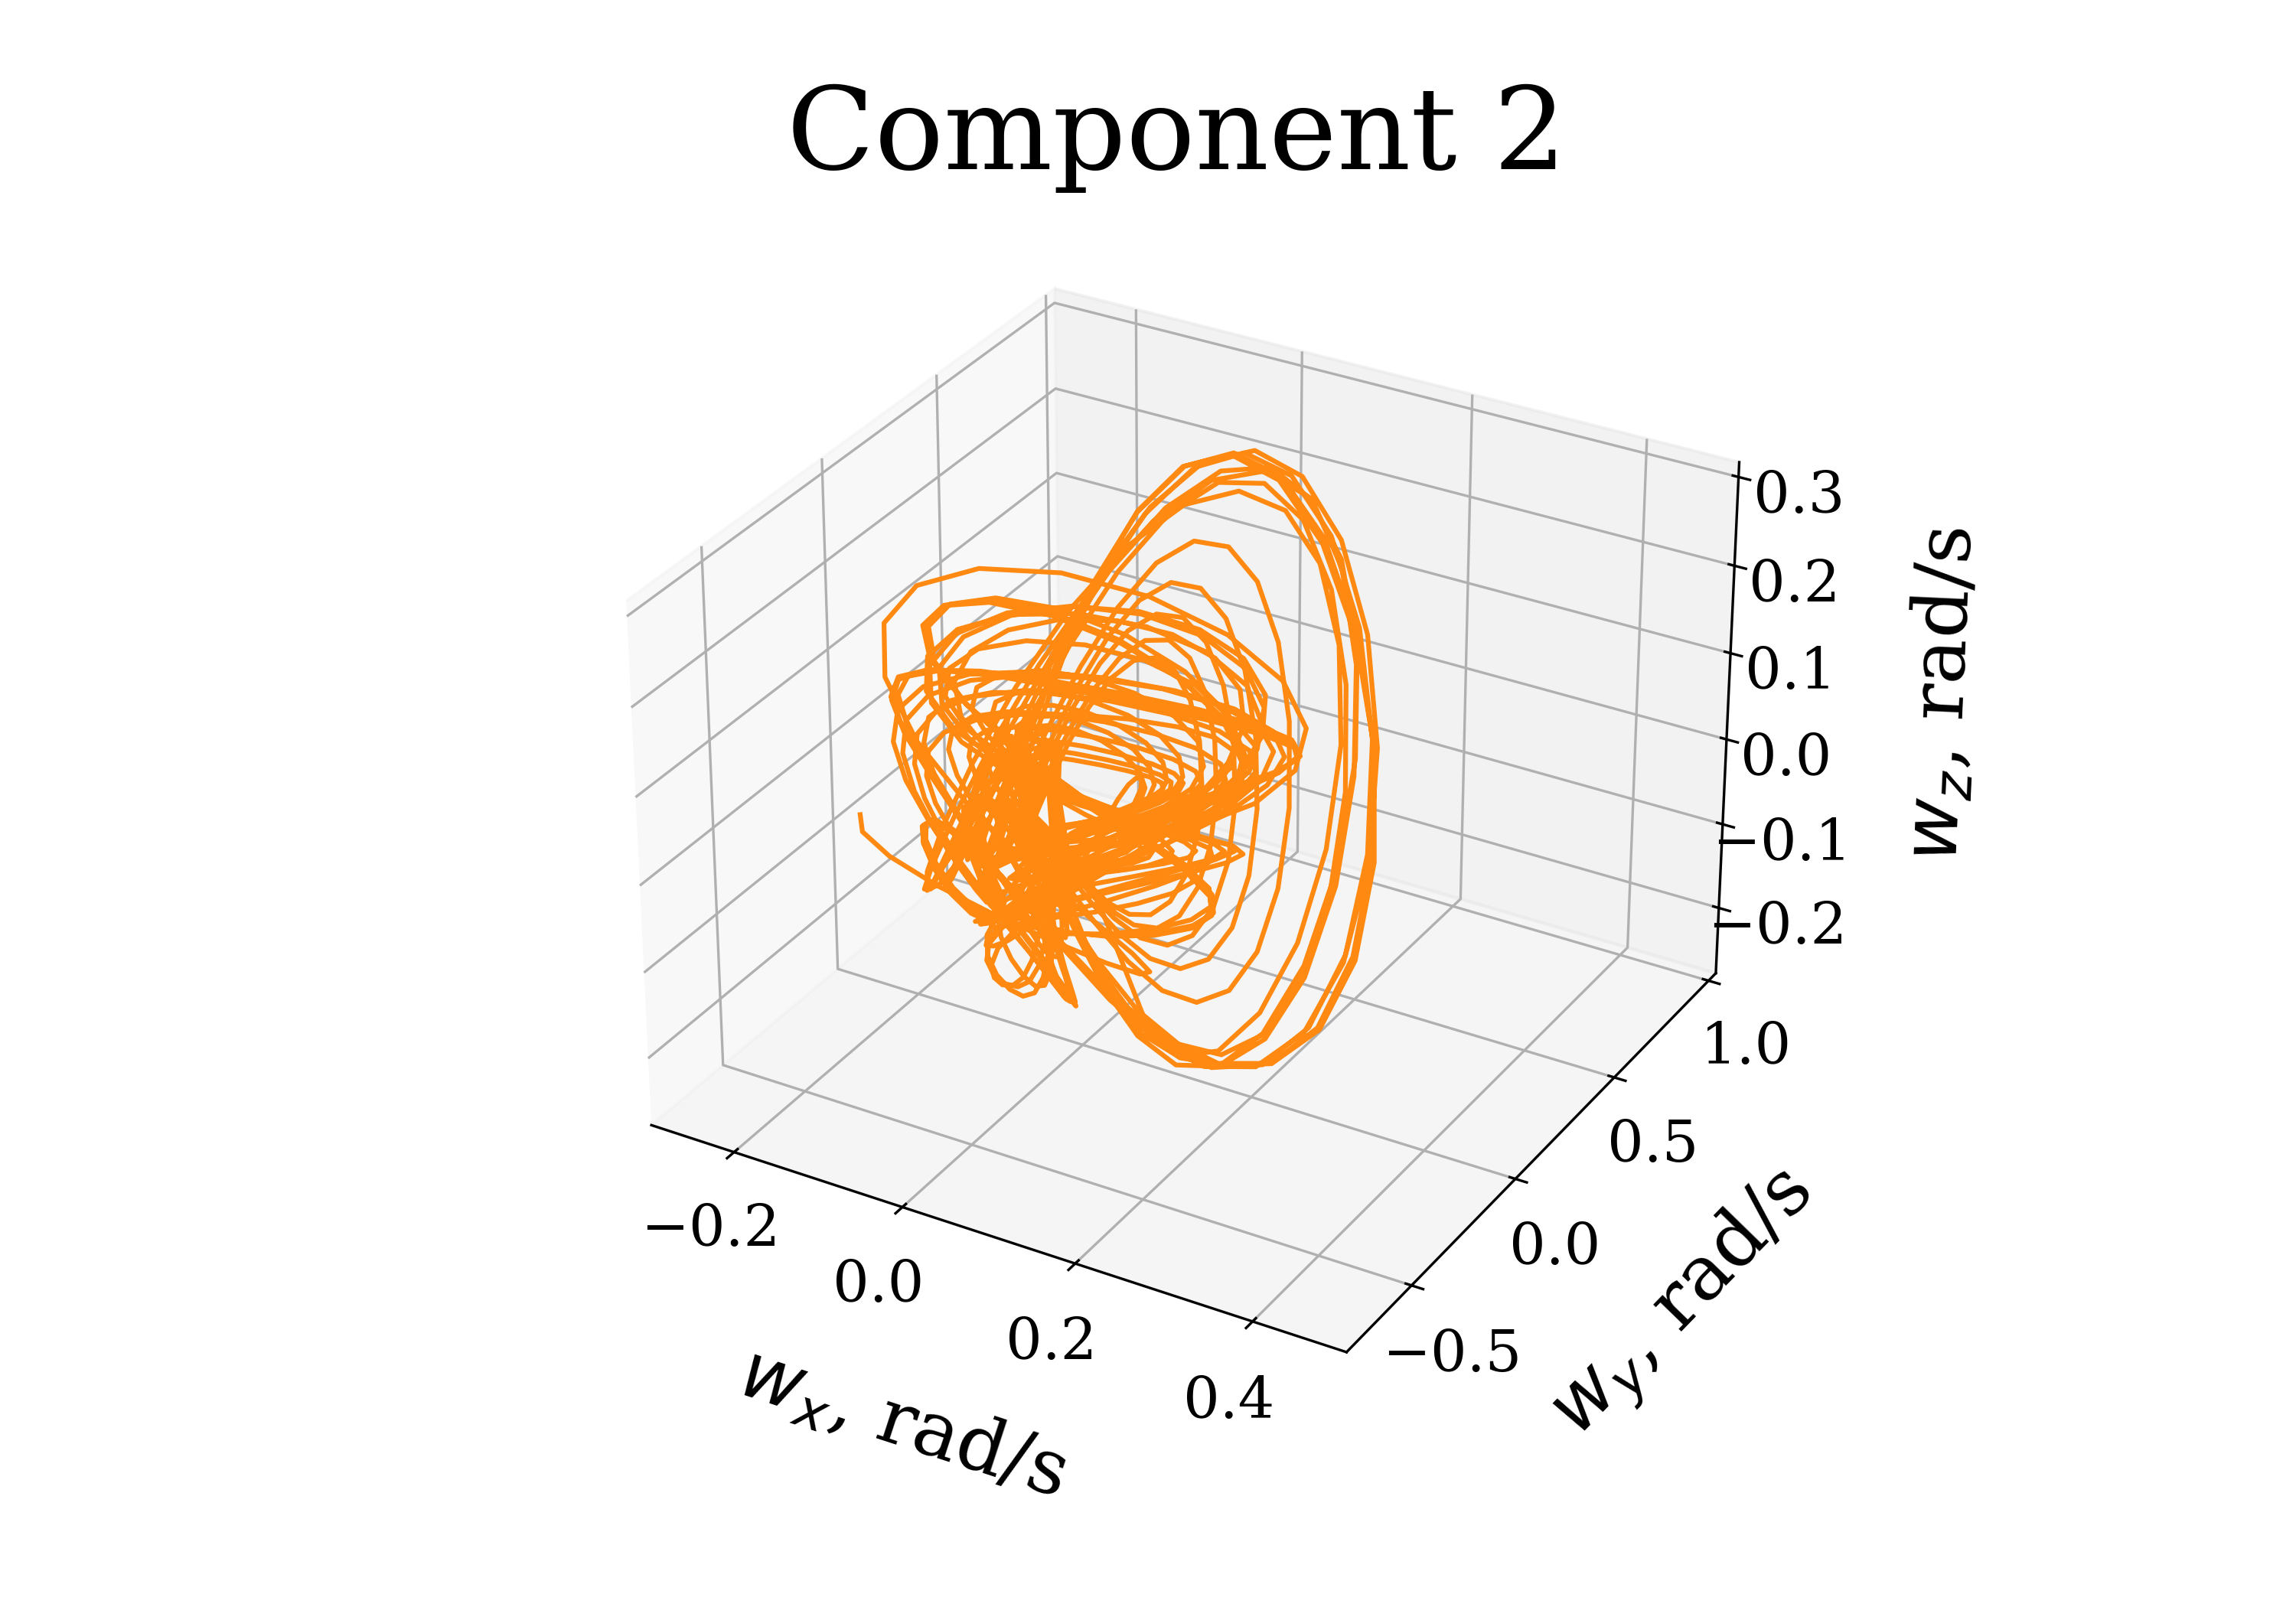
\includegraphics[width=0.48\textwidth, keepaspectratio]{gyro_2.png}
		\caption{tSSA decomposition for the gyroscope data. CPD rank $ = 10 $}\label{fig:gyro_decomp_tssa}
	\end{figure}
	
	We also present the mSSA's decomposition for the electricity data in the Fig. \ref{fig:electr_decomp_mssa} and for the inertial unit data in the Fig. \ref{fig:accel_decomp_mssa}, \ref{fig:gyro_decomp_mssa}. The decomposition here is similar to the tSSA and connected with the factors partitioning. Several heuristics exist to make the partitioning manually~\cite{ecfb9dc578be43ae9ee8fc88b8ff9151}. As shown in the Tab. \ref{tab:decomp_electr_results} and \ref{tab:decomp_motion_results}, the decomposition metrics are greater for that heuristics then for the tSSA. Number of the mSSA's components is not limited. However, such results are not always guaranteed. Automation here is hindered. Moreover, the mSSA's components for the inertial unit data are trivial and do not reflect complex dynamics of the mechanical motion. To summarize, the complexity of the tSSA decomposition does not allow for building many components but guarantees their optimal quality in terms of the AHE and RHE.
	
	\begin{figure}[h]
		\centering
		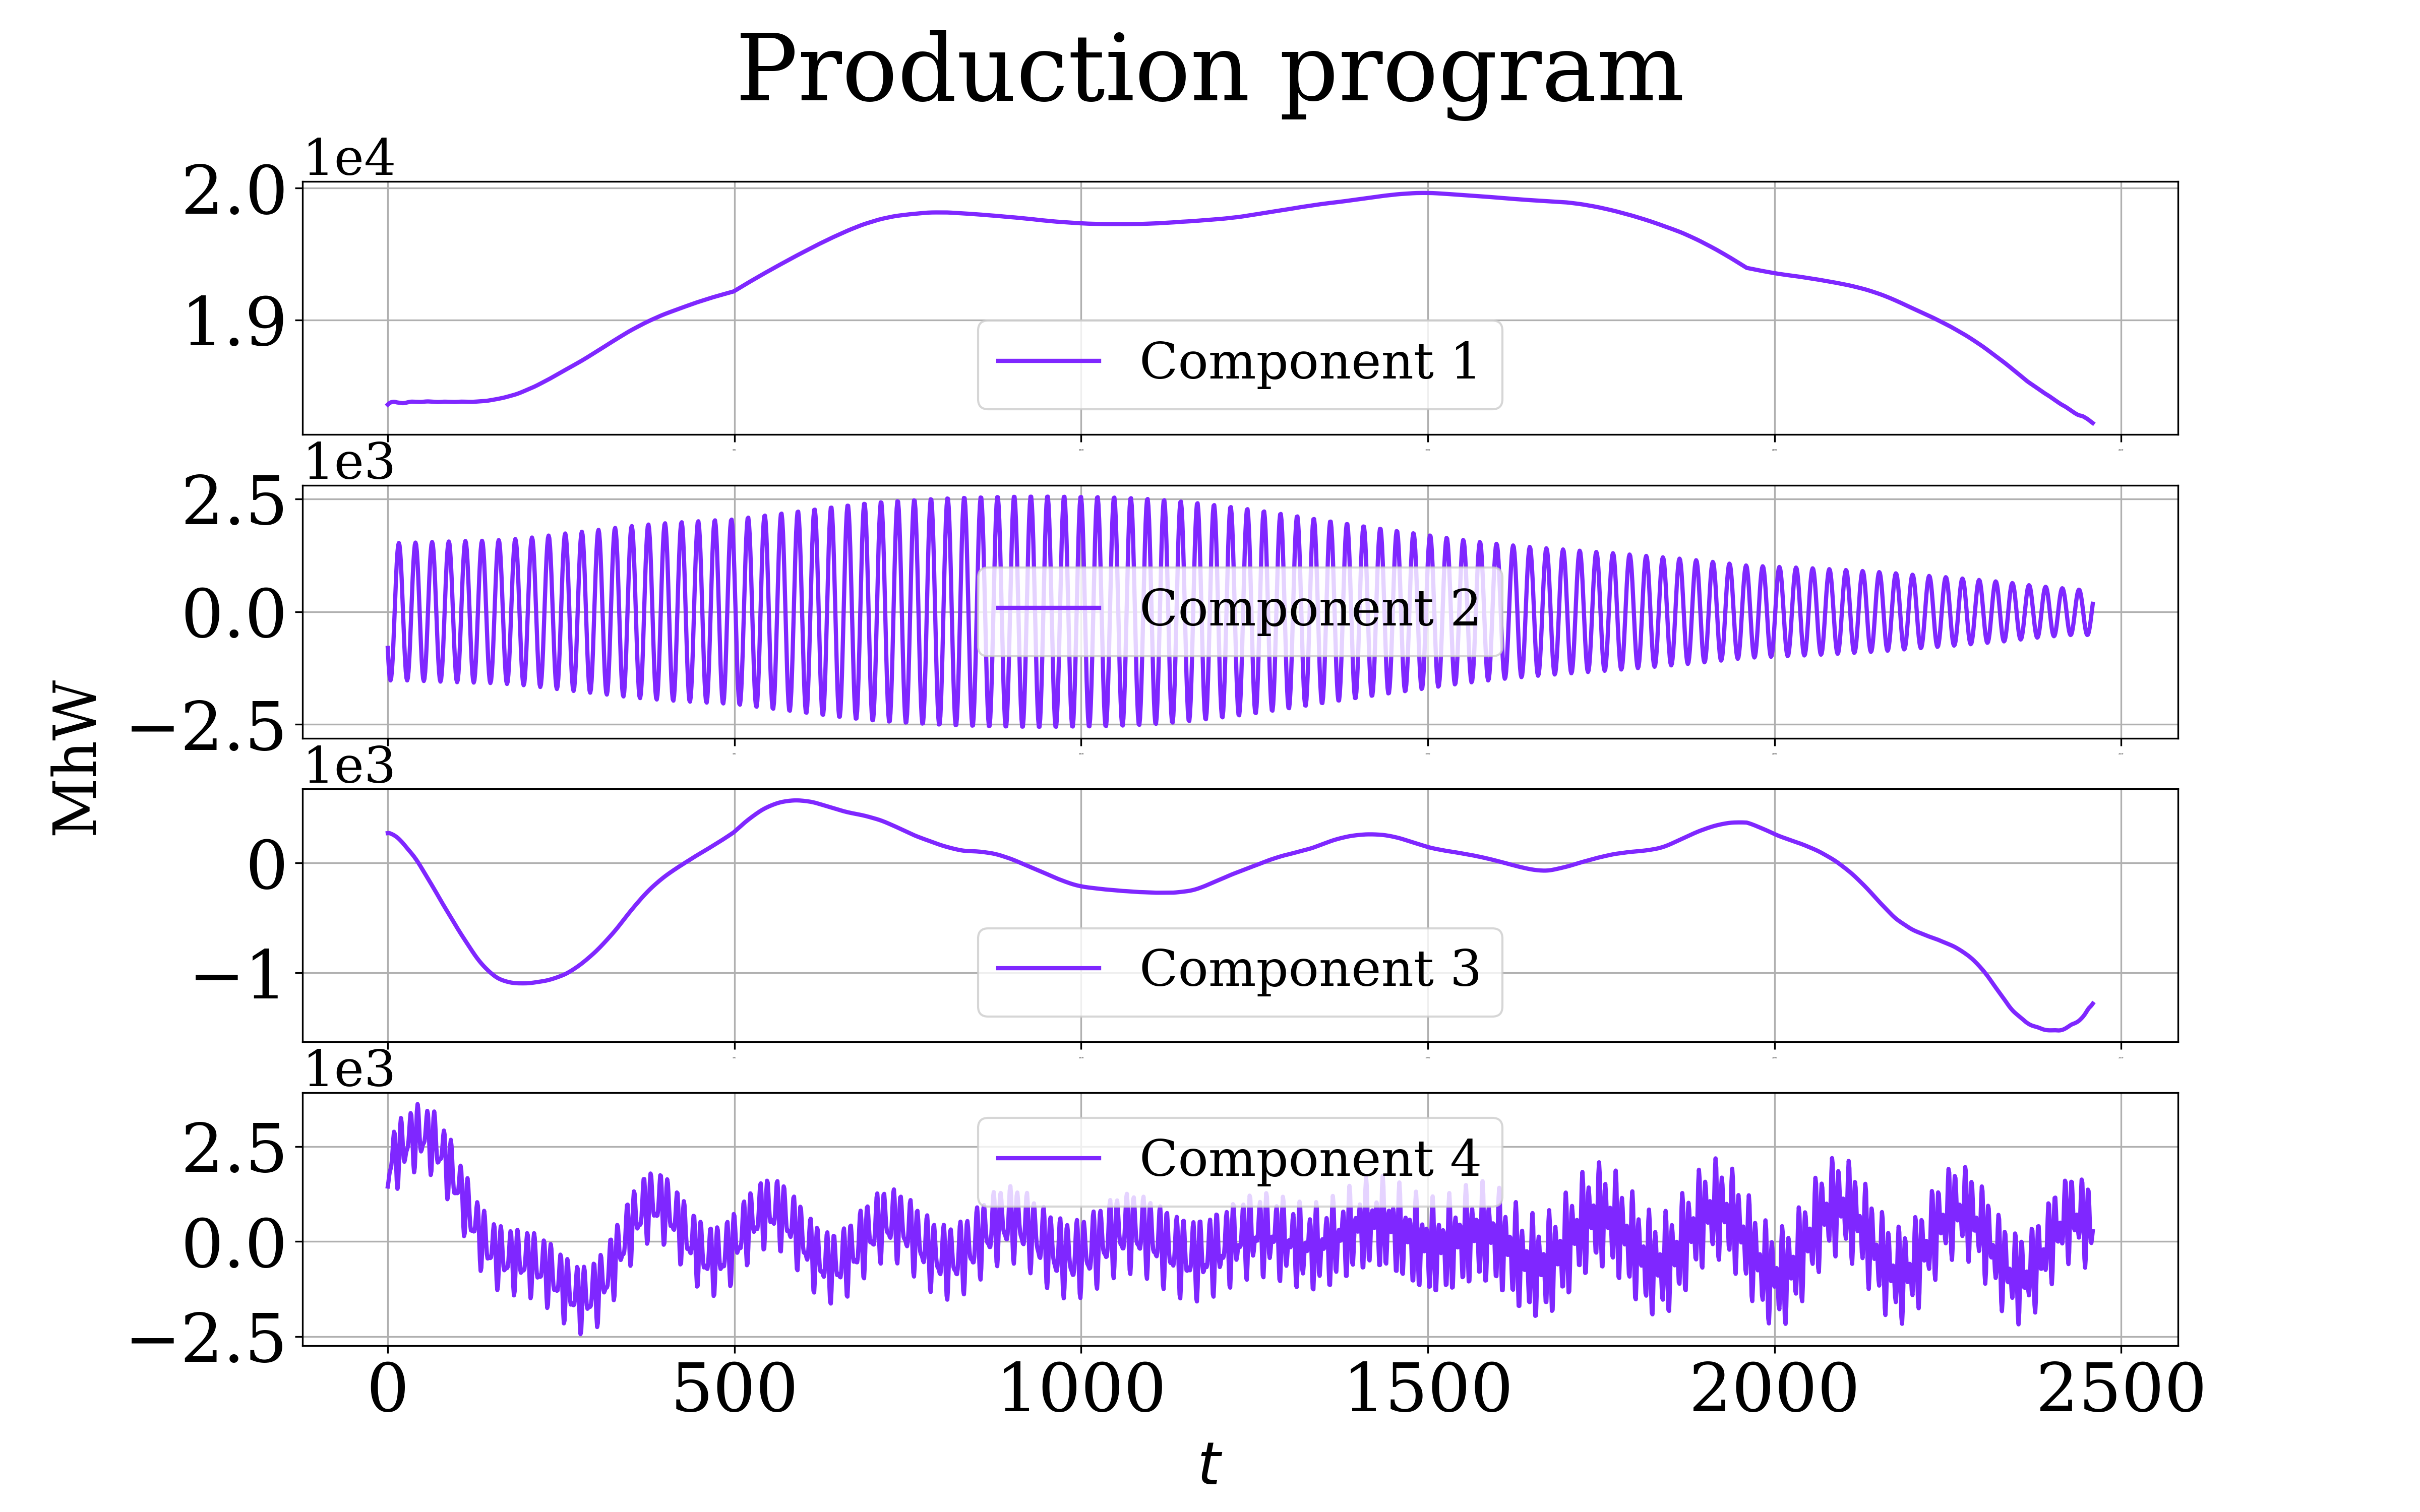
\includegraphics[width=0.48\textwidth, keepaspectratio]{Production_program_mssa.png}
		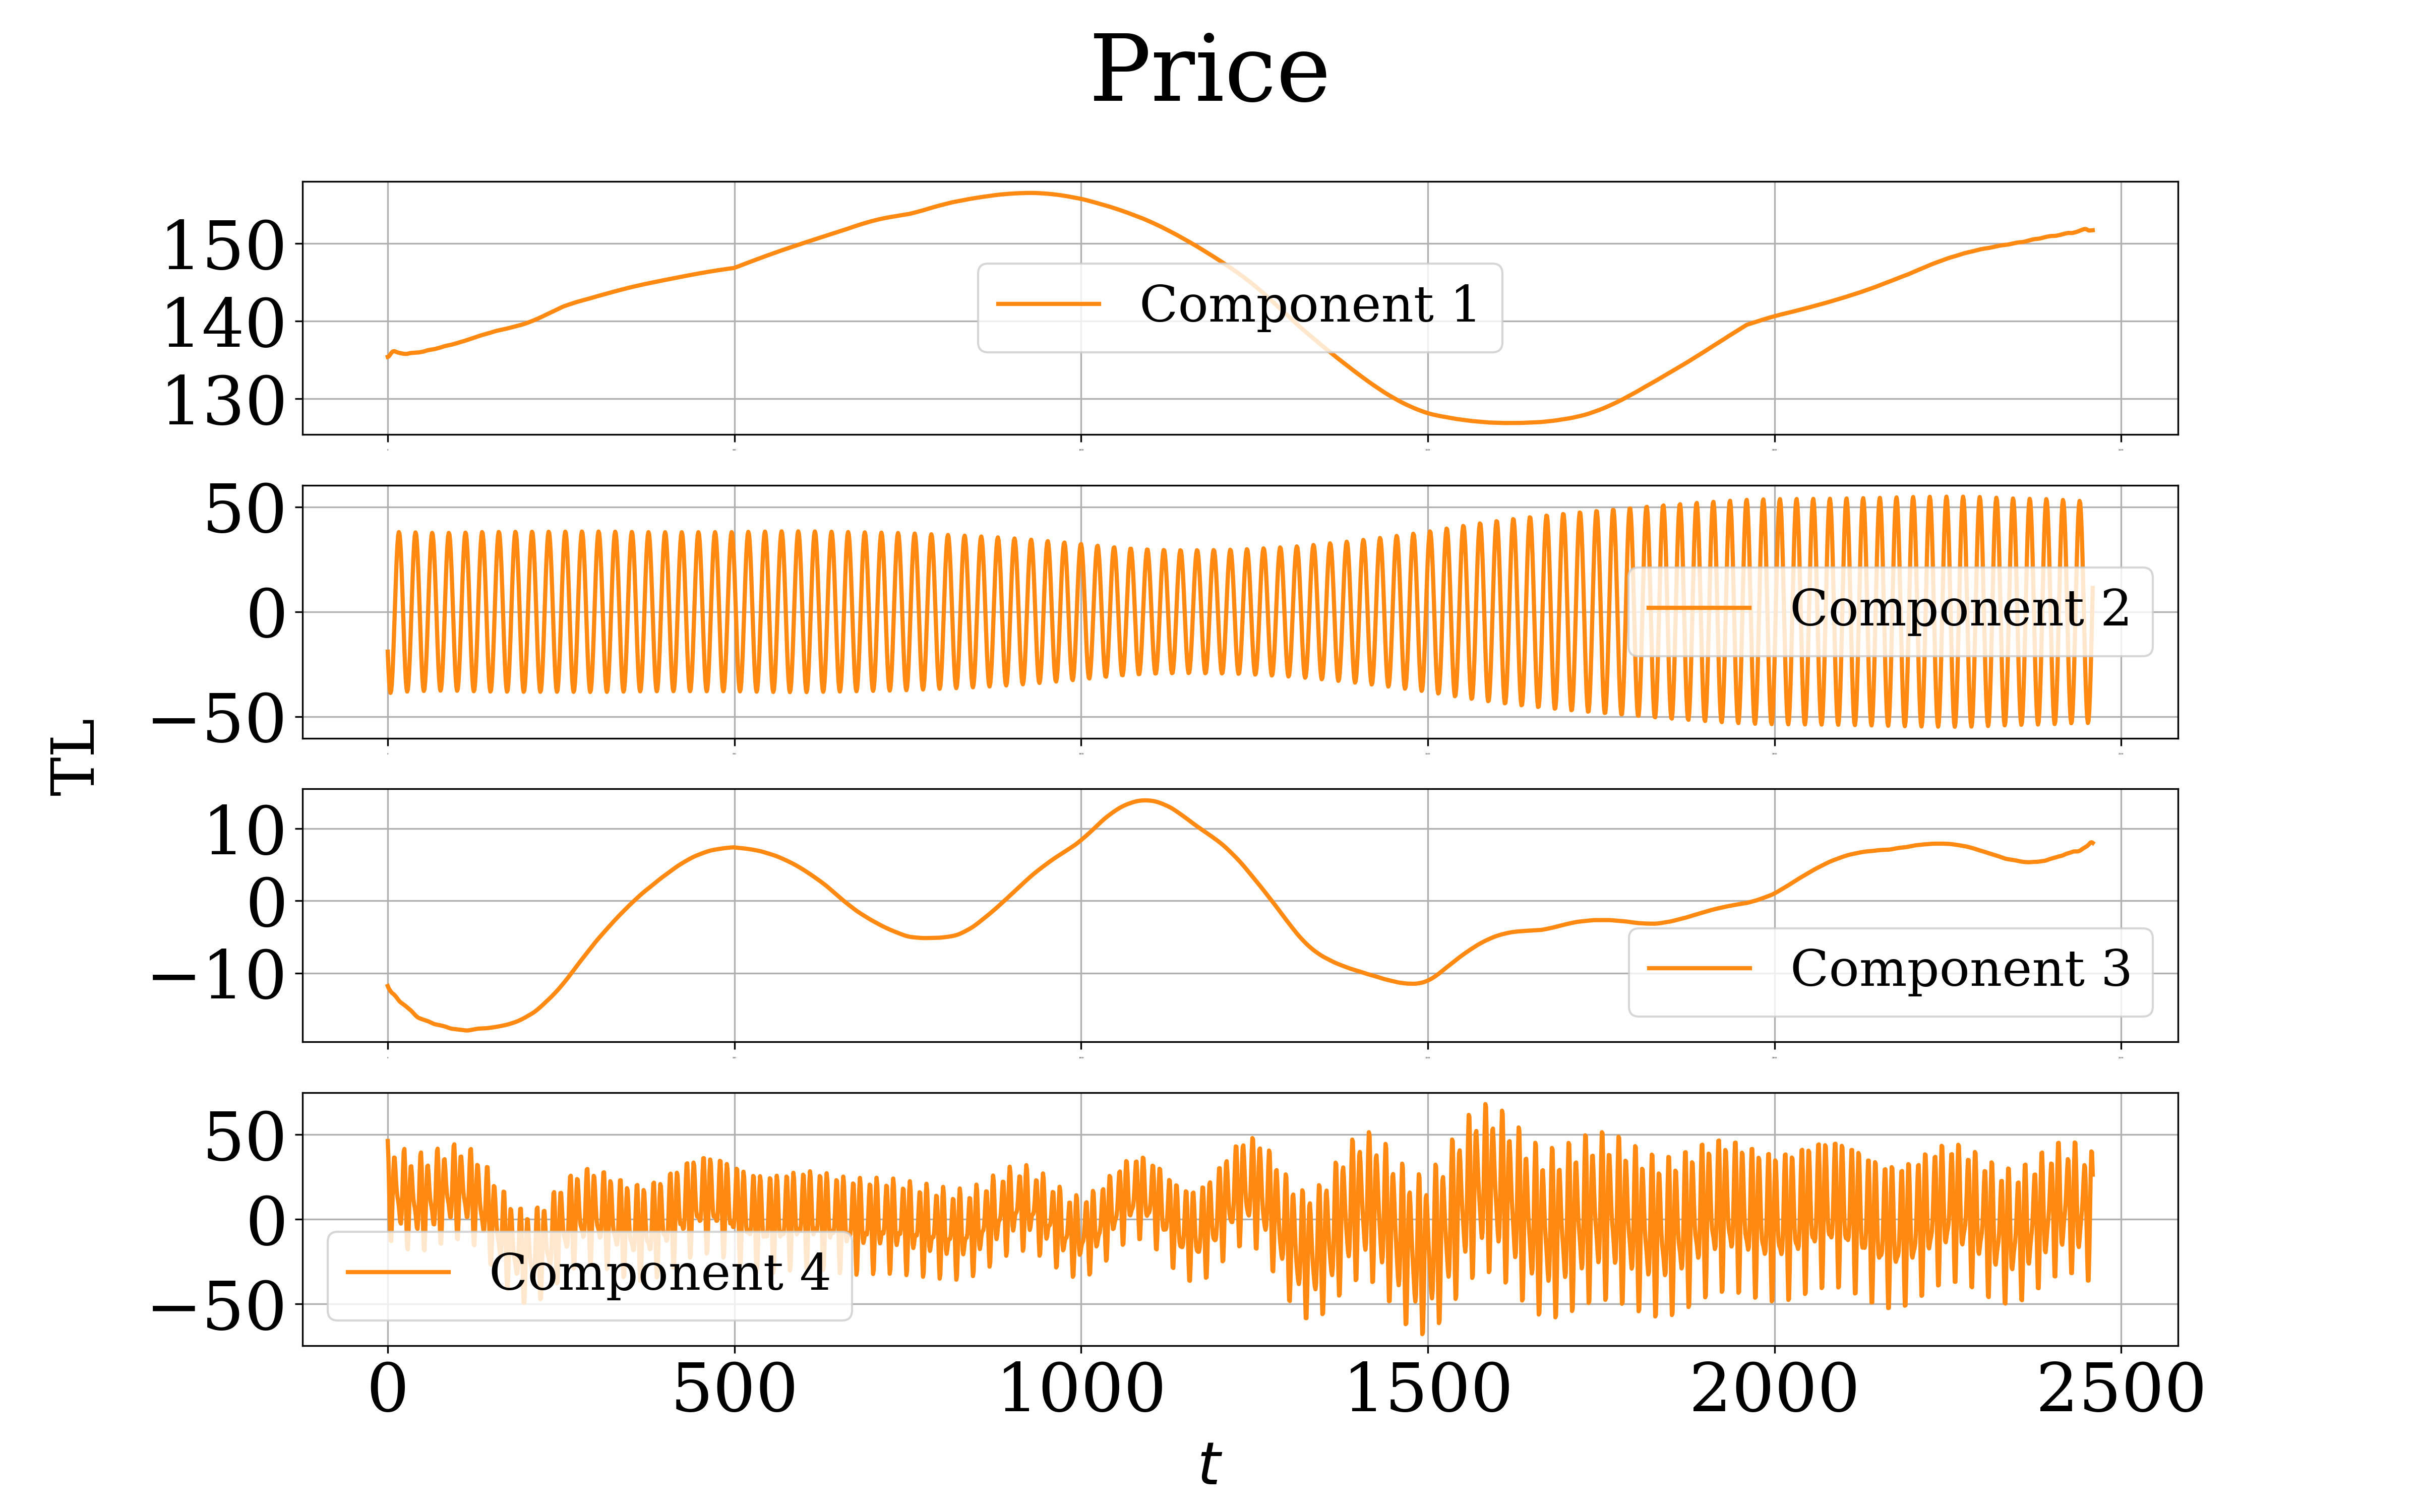
\includegraphics[width=0.48\textwidth, keepaspectratio]{Price_mssa.png}
		\caption{mSSA decomposition for the electricity data}\label{fig:electr_decomp_mssa}
	\end{figure}
	
	\begin{figure}[h]
		\centering
		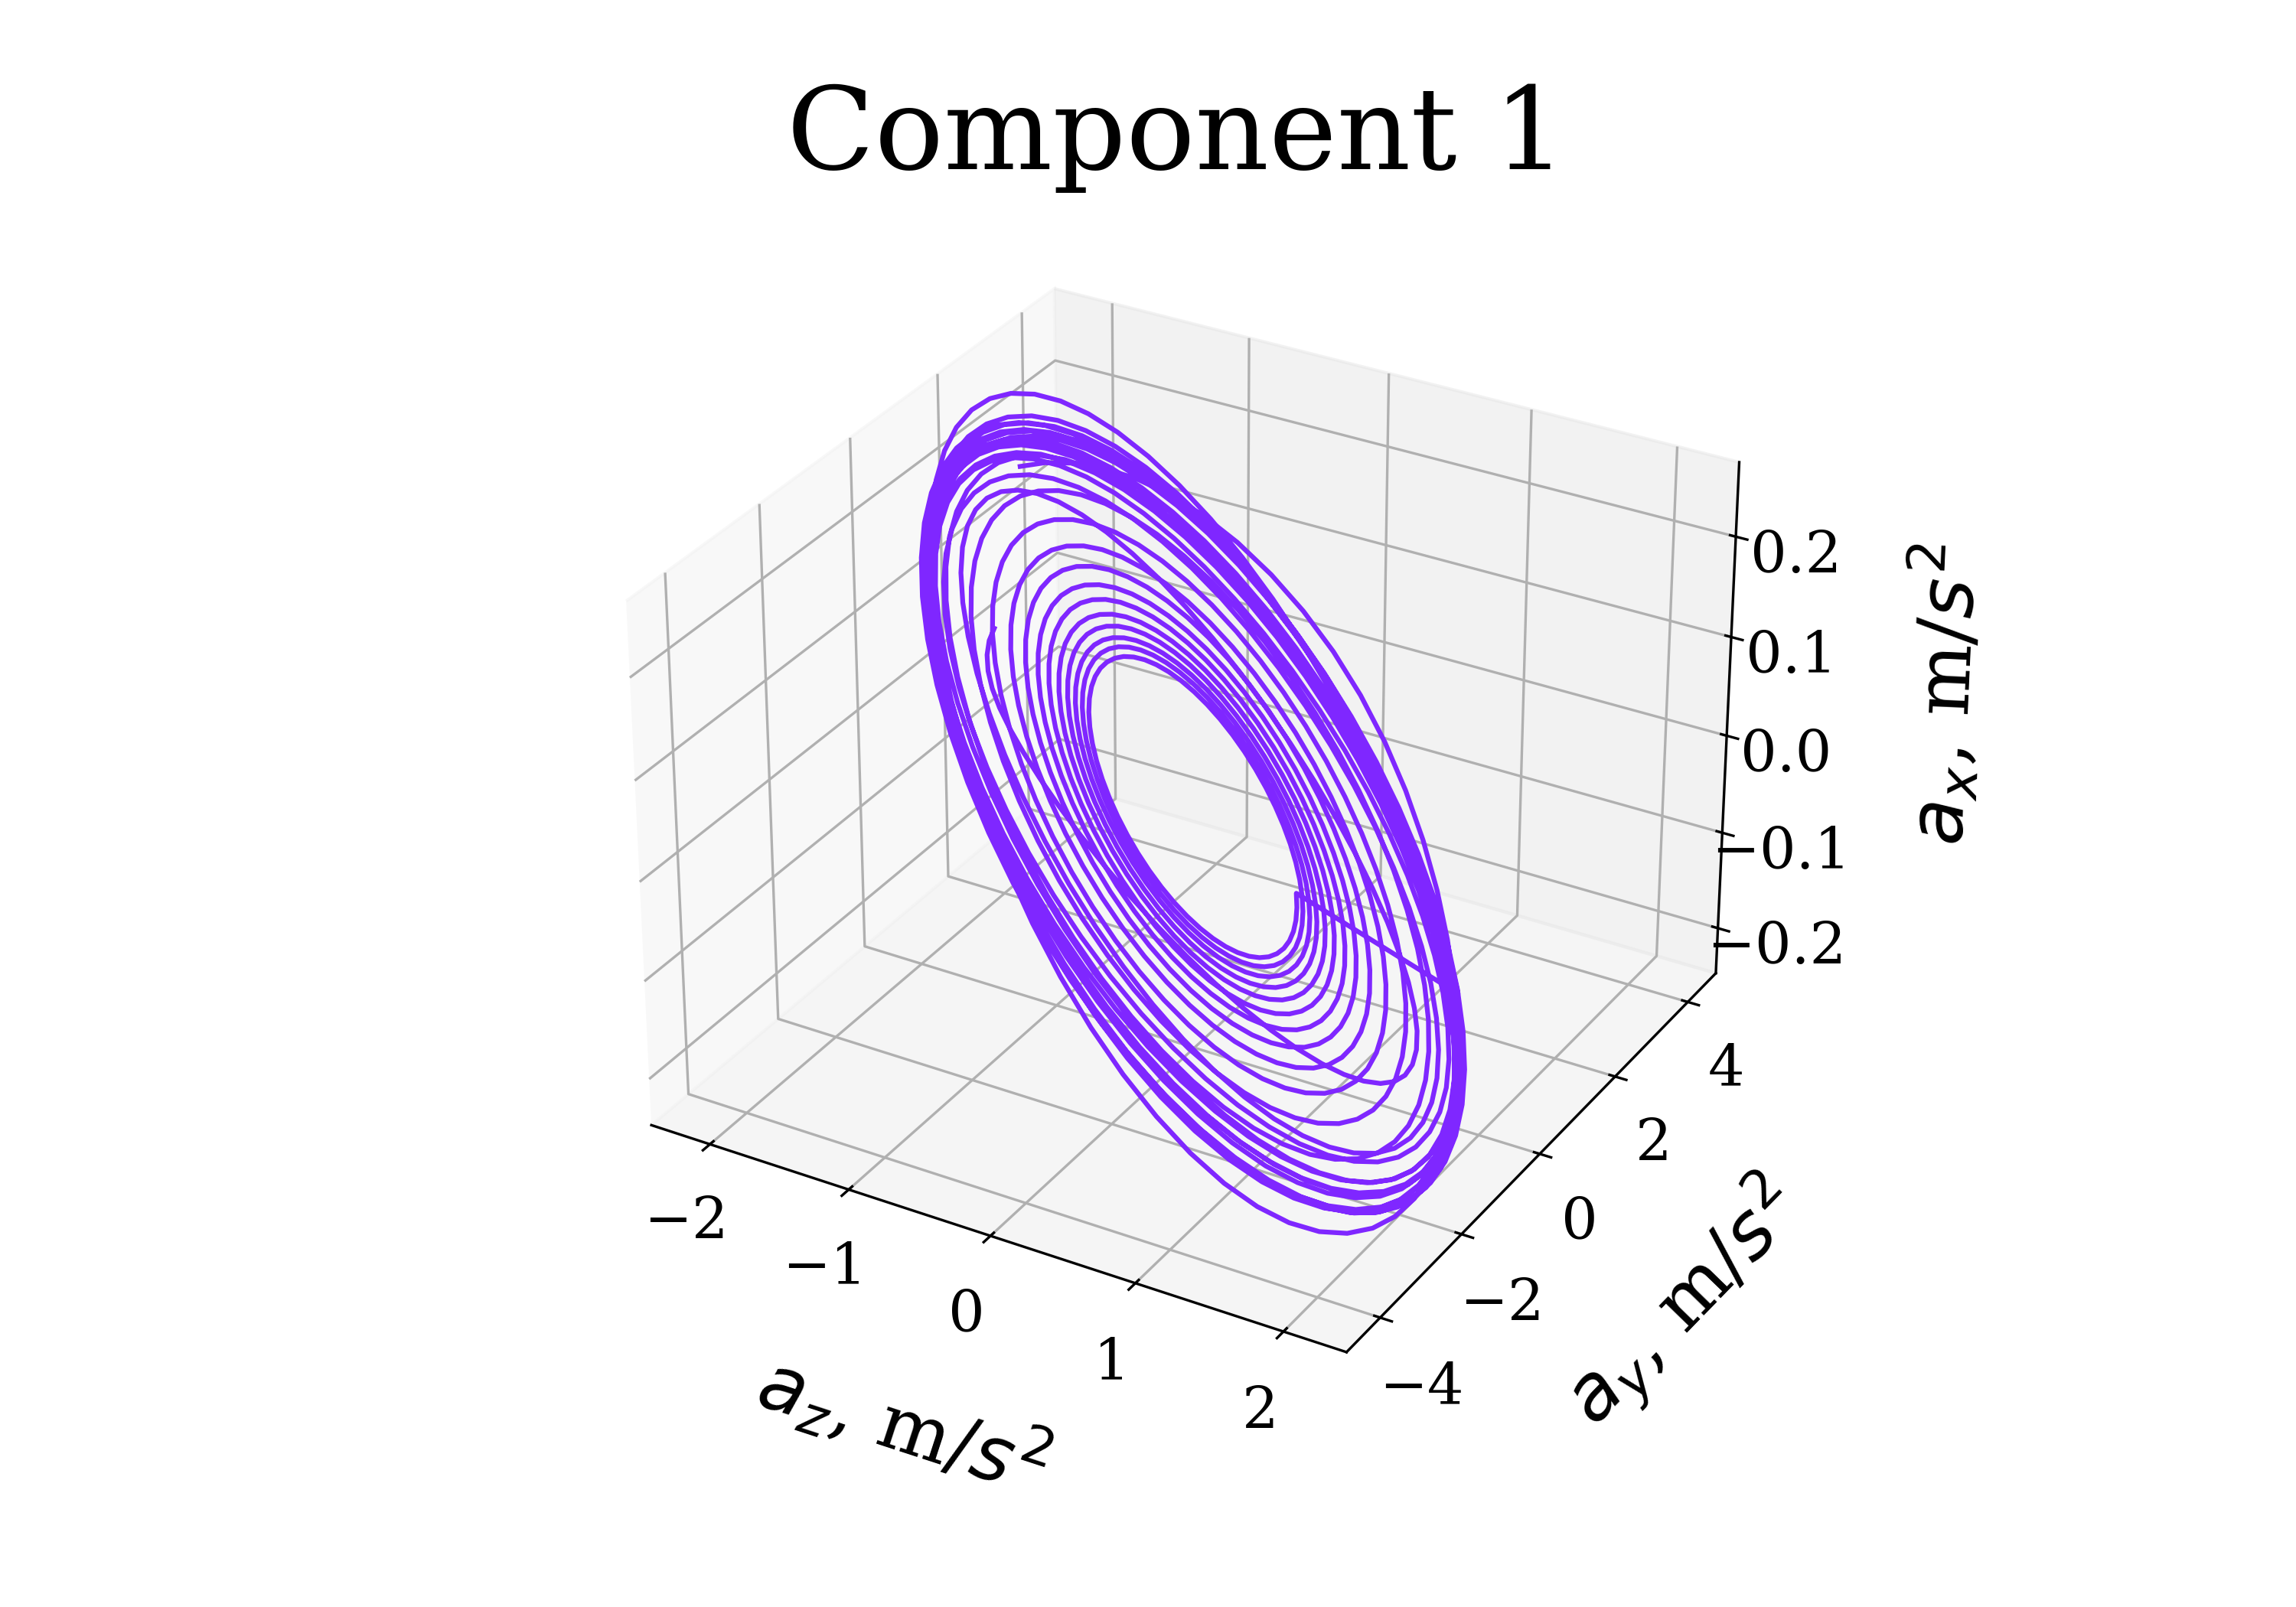
\includegraphics[width=0.48\textwidth, keepaspectratio]{acceler_1_mssa.png}
		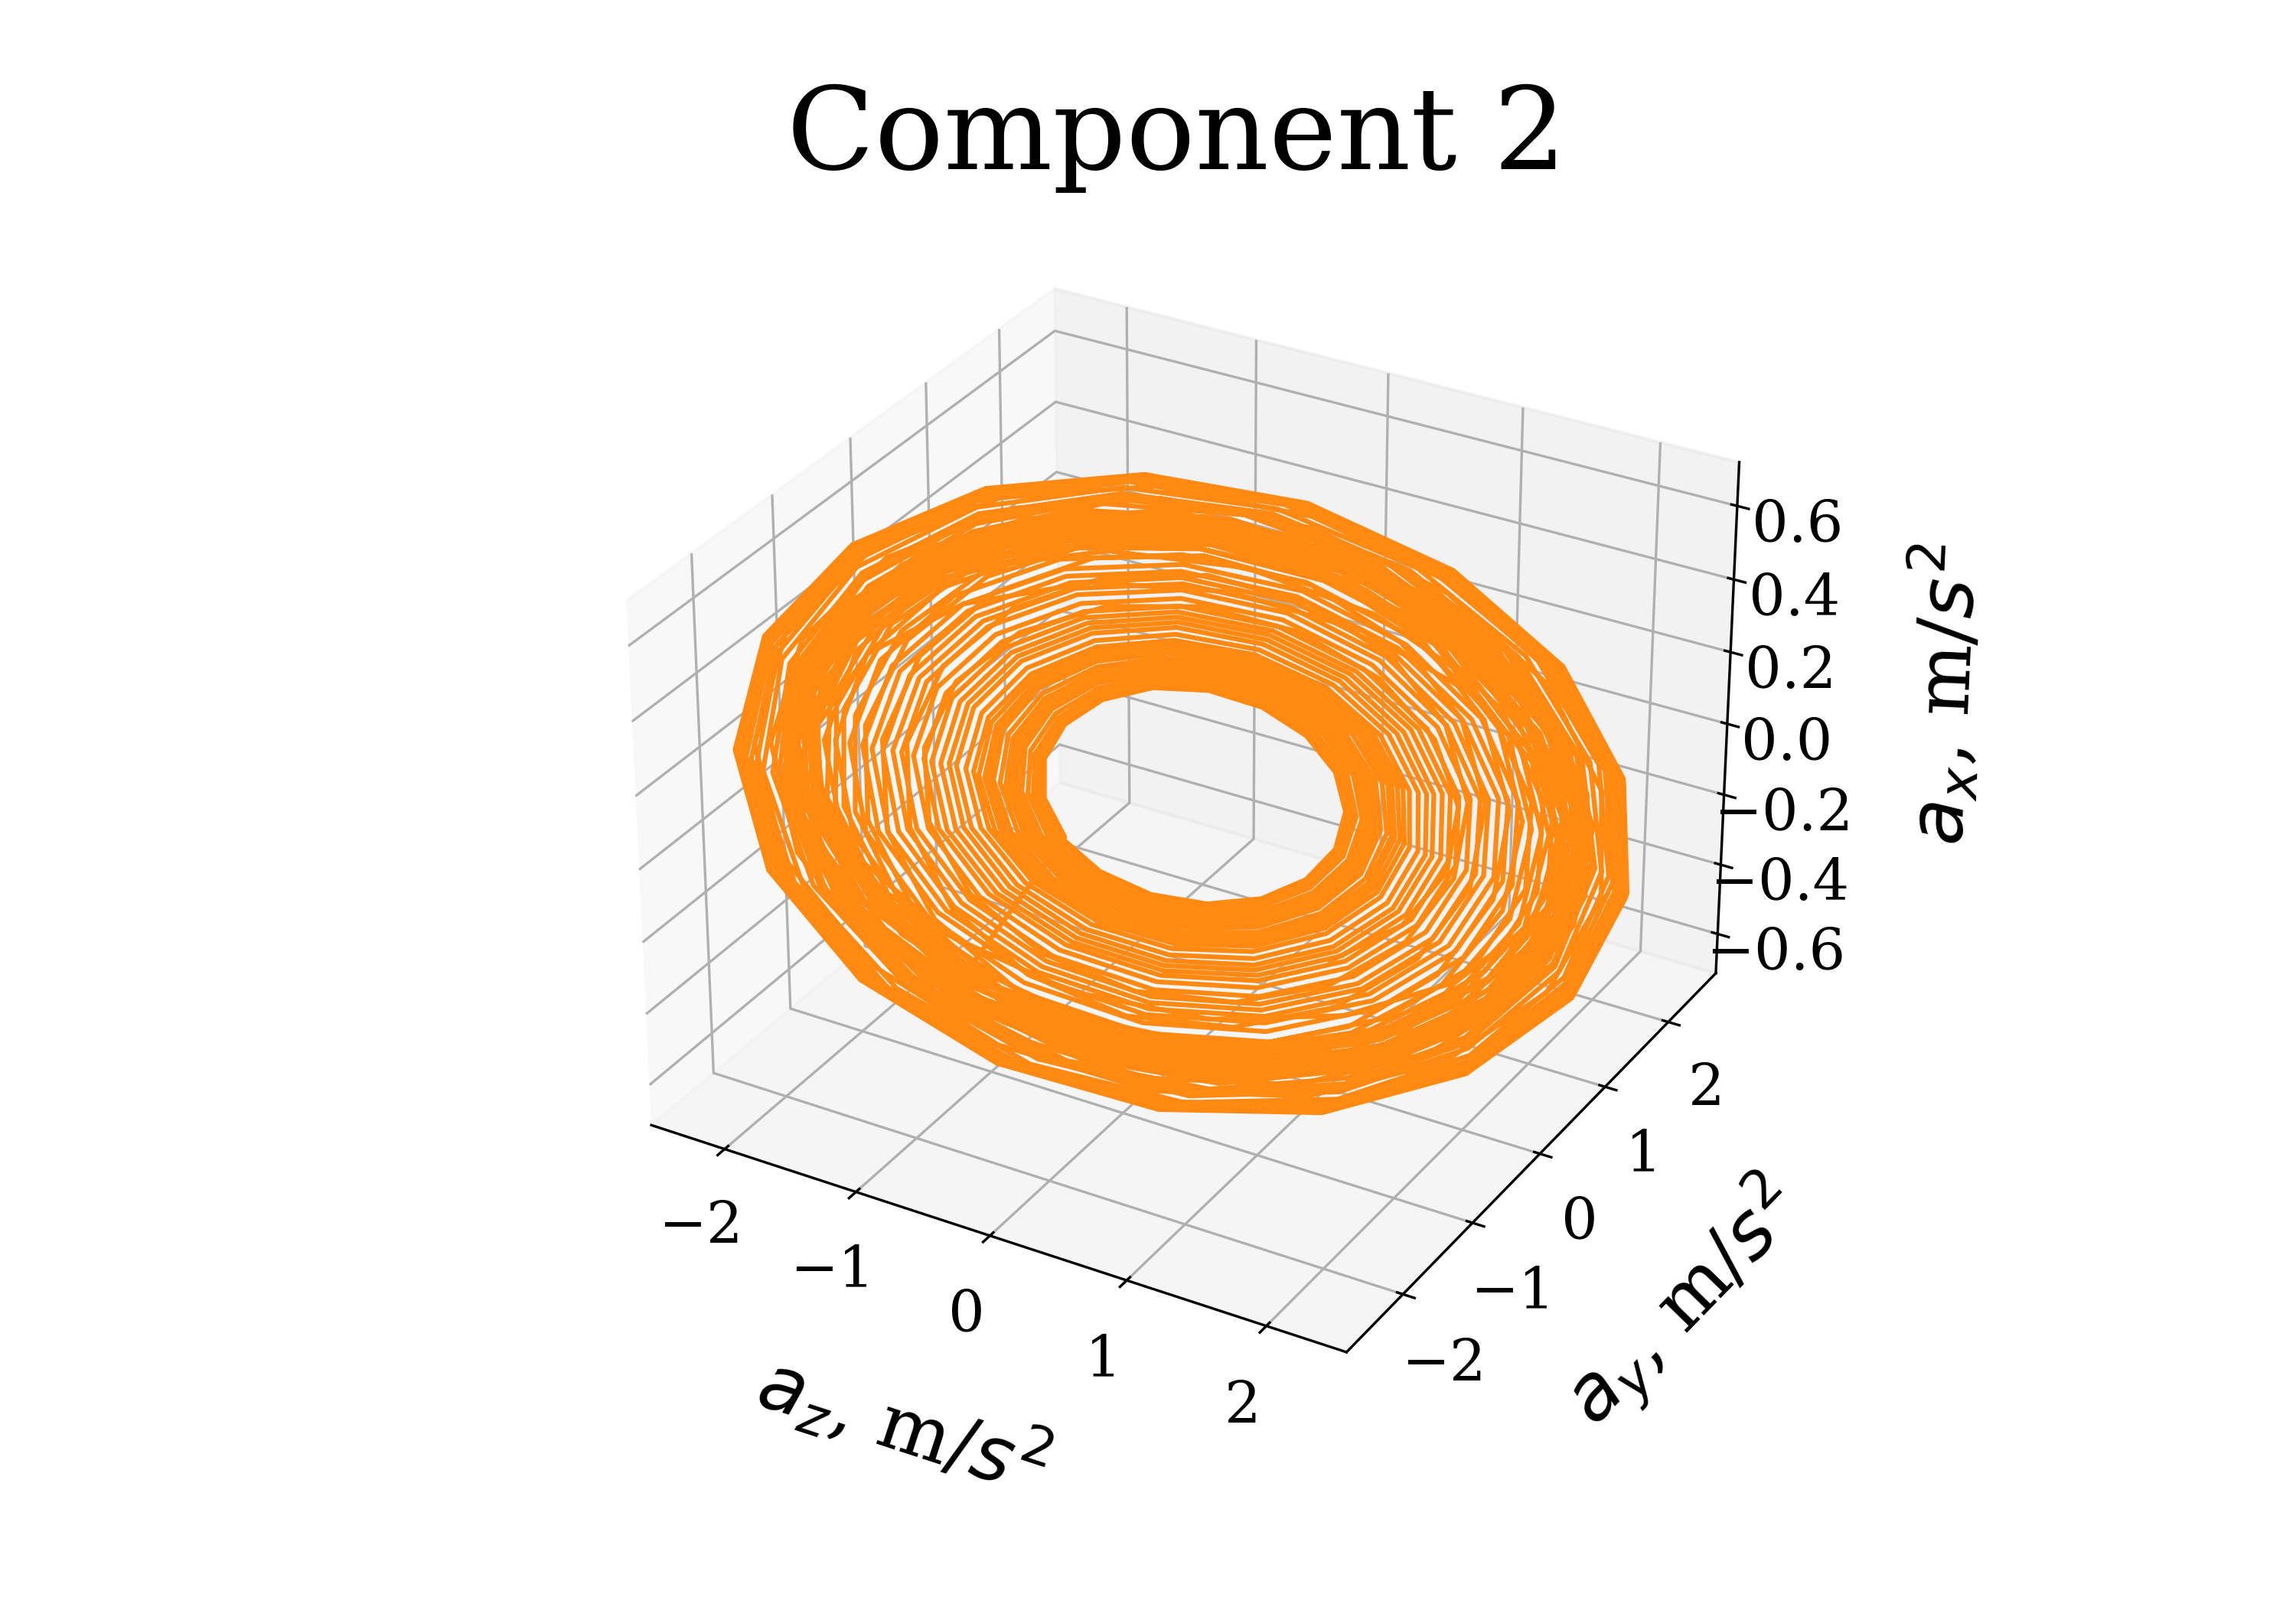
\includegraphics[width=0.48\textwidth, keepaspectratio]{acceler_2_mssa.png}
		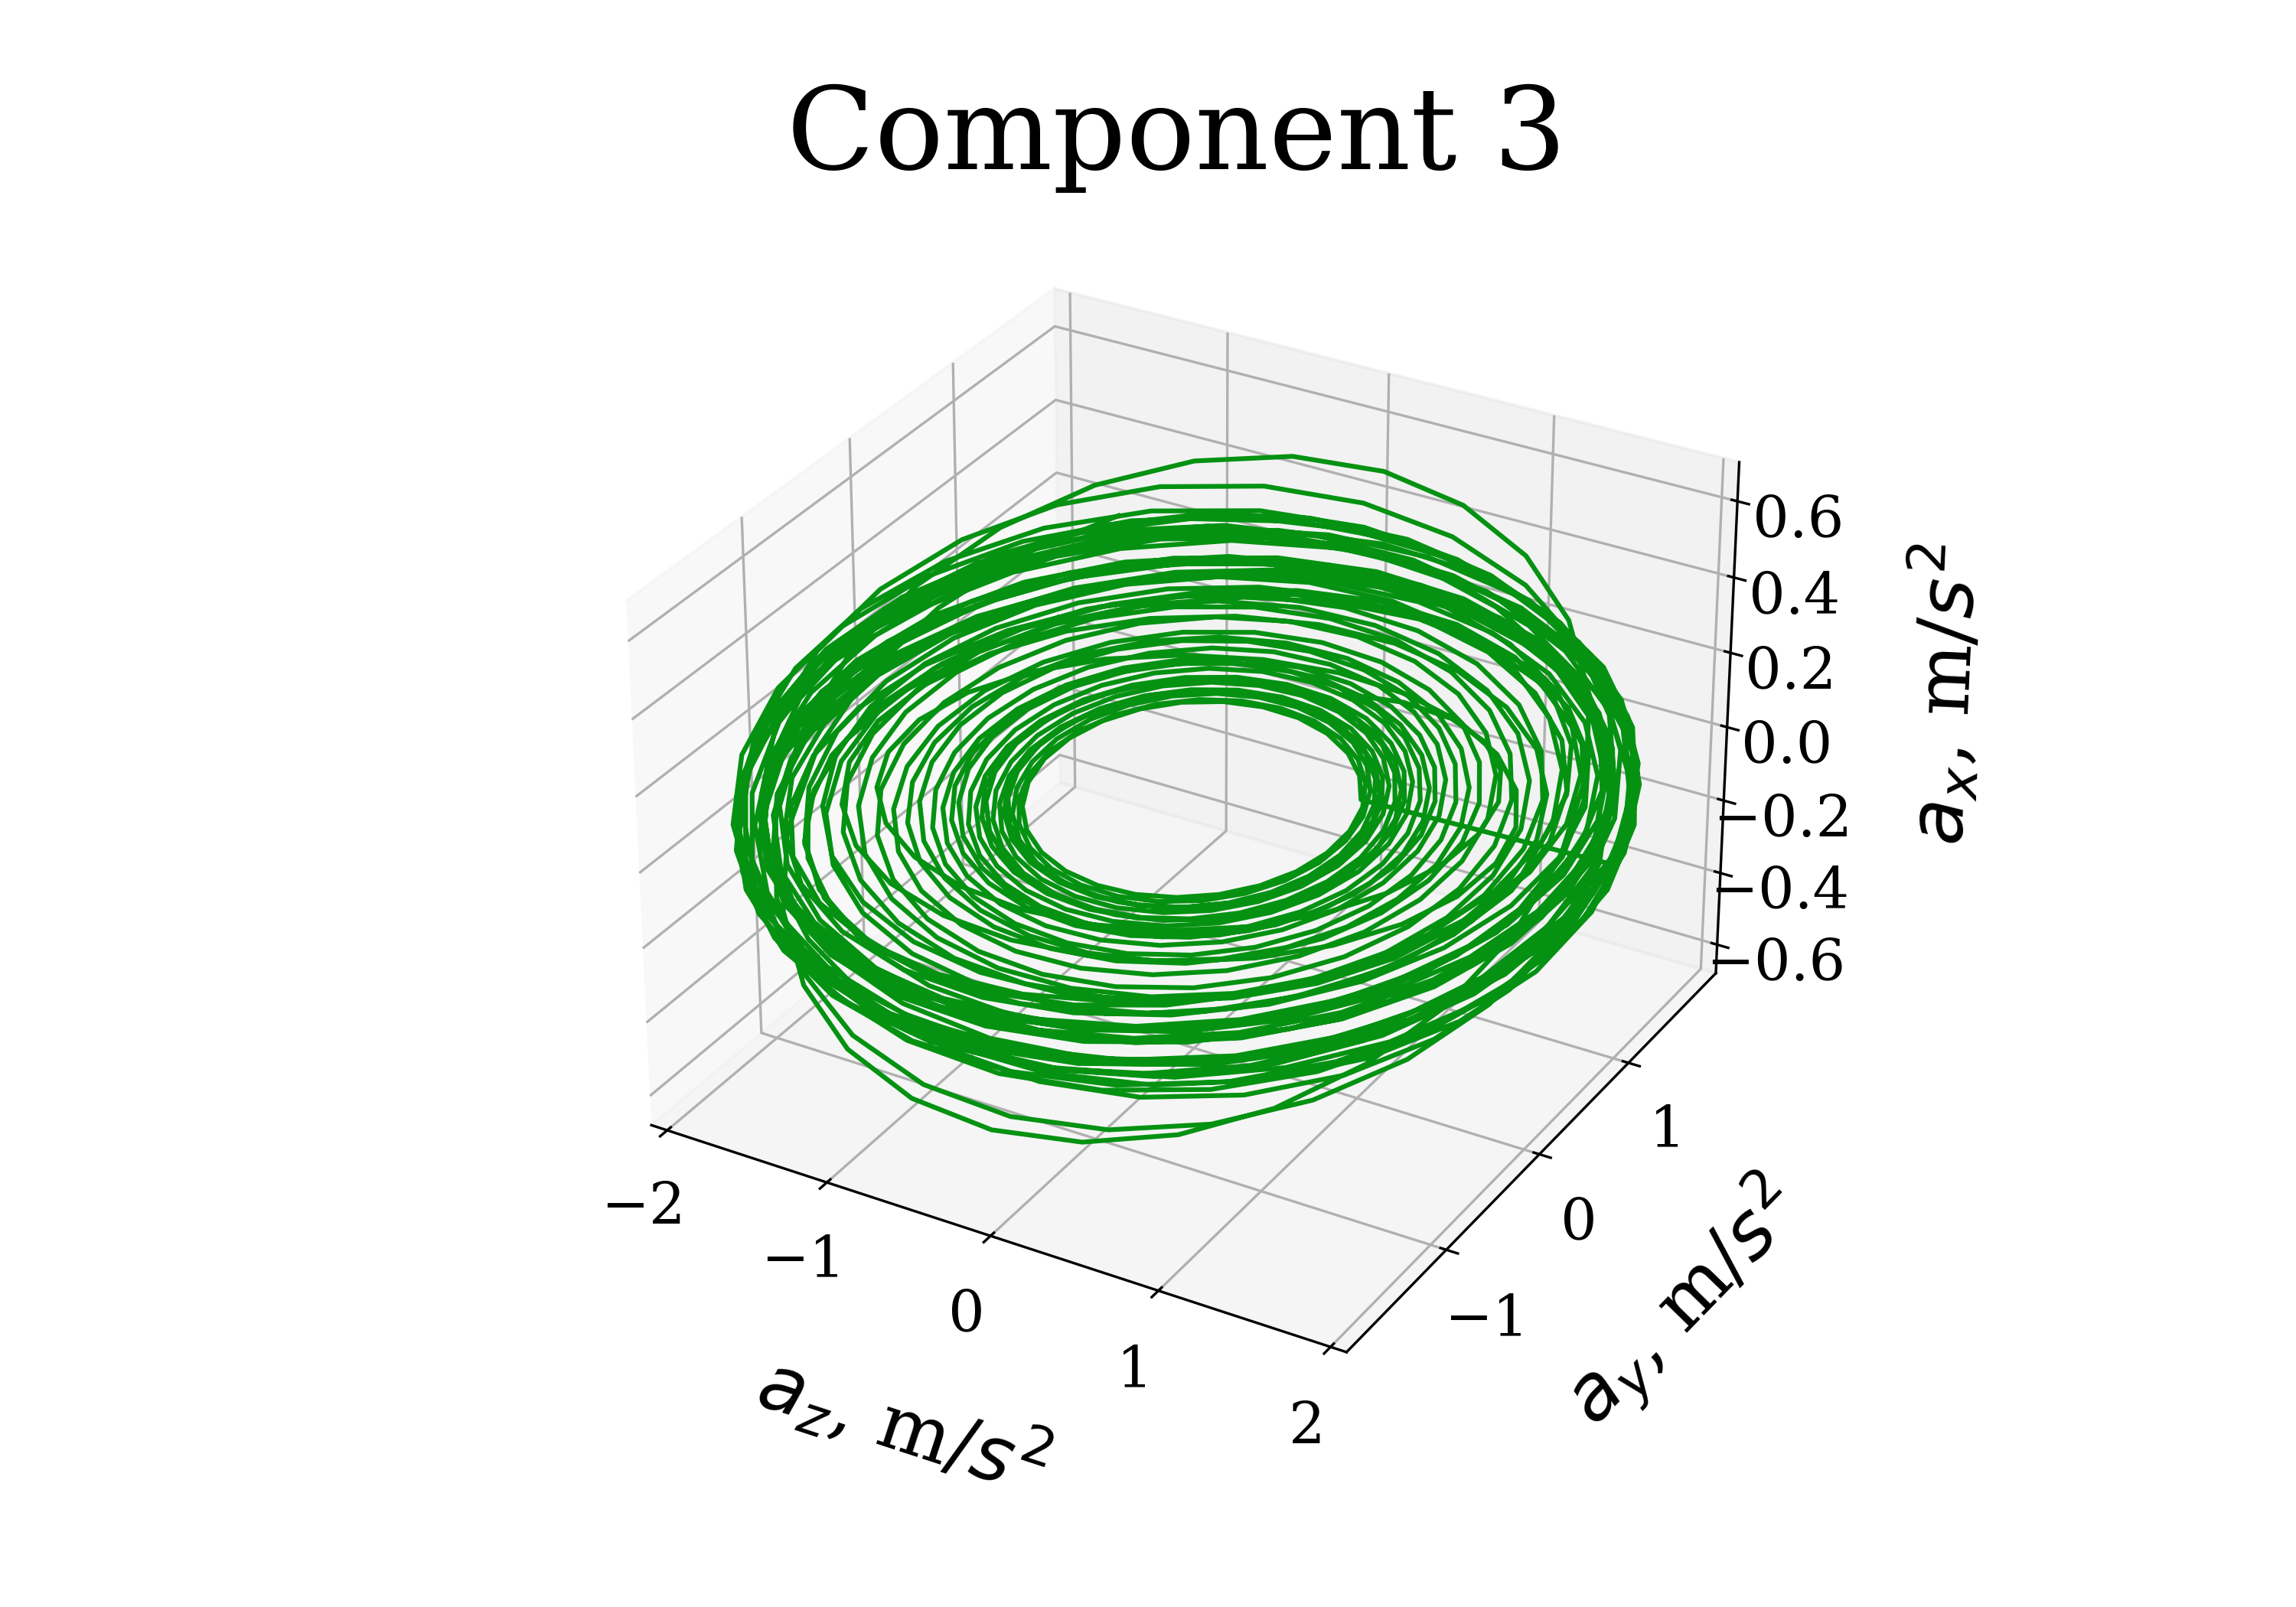
\includegraphics[width=0.48\textwidth, keepaspectratio]{acceler_3_mssa.png}
		\caption{mSSA decomposition for the accelerometer data}\label{fig:accel_decomp_mssa}
	\end{figure}
	
	\begin{figure}[h]
		\centering
		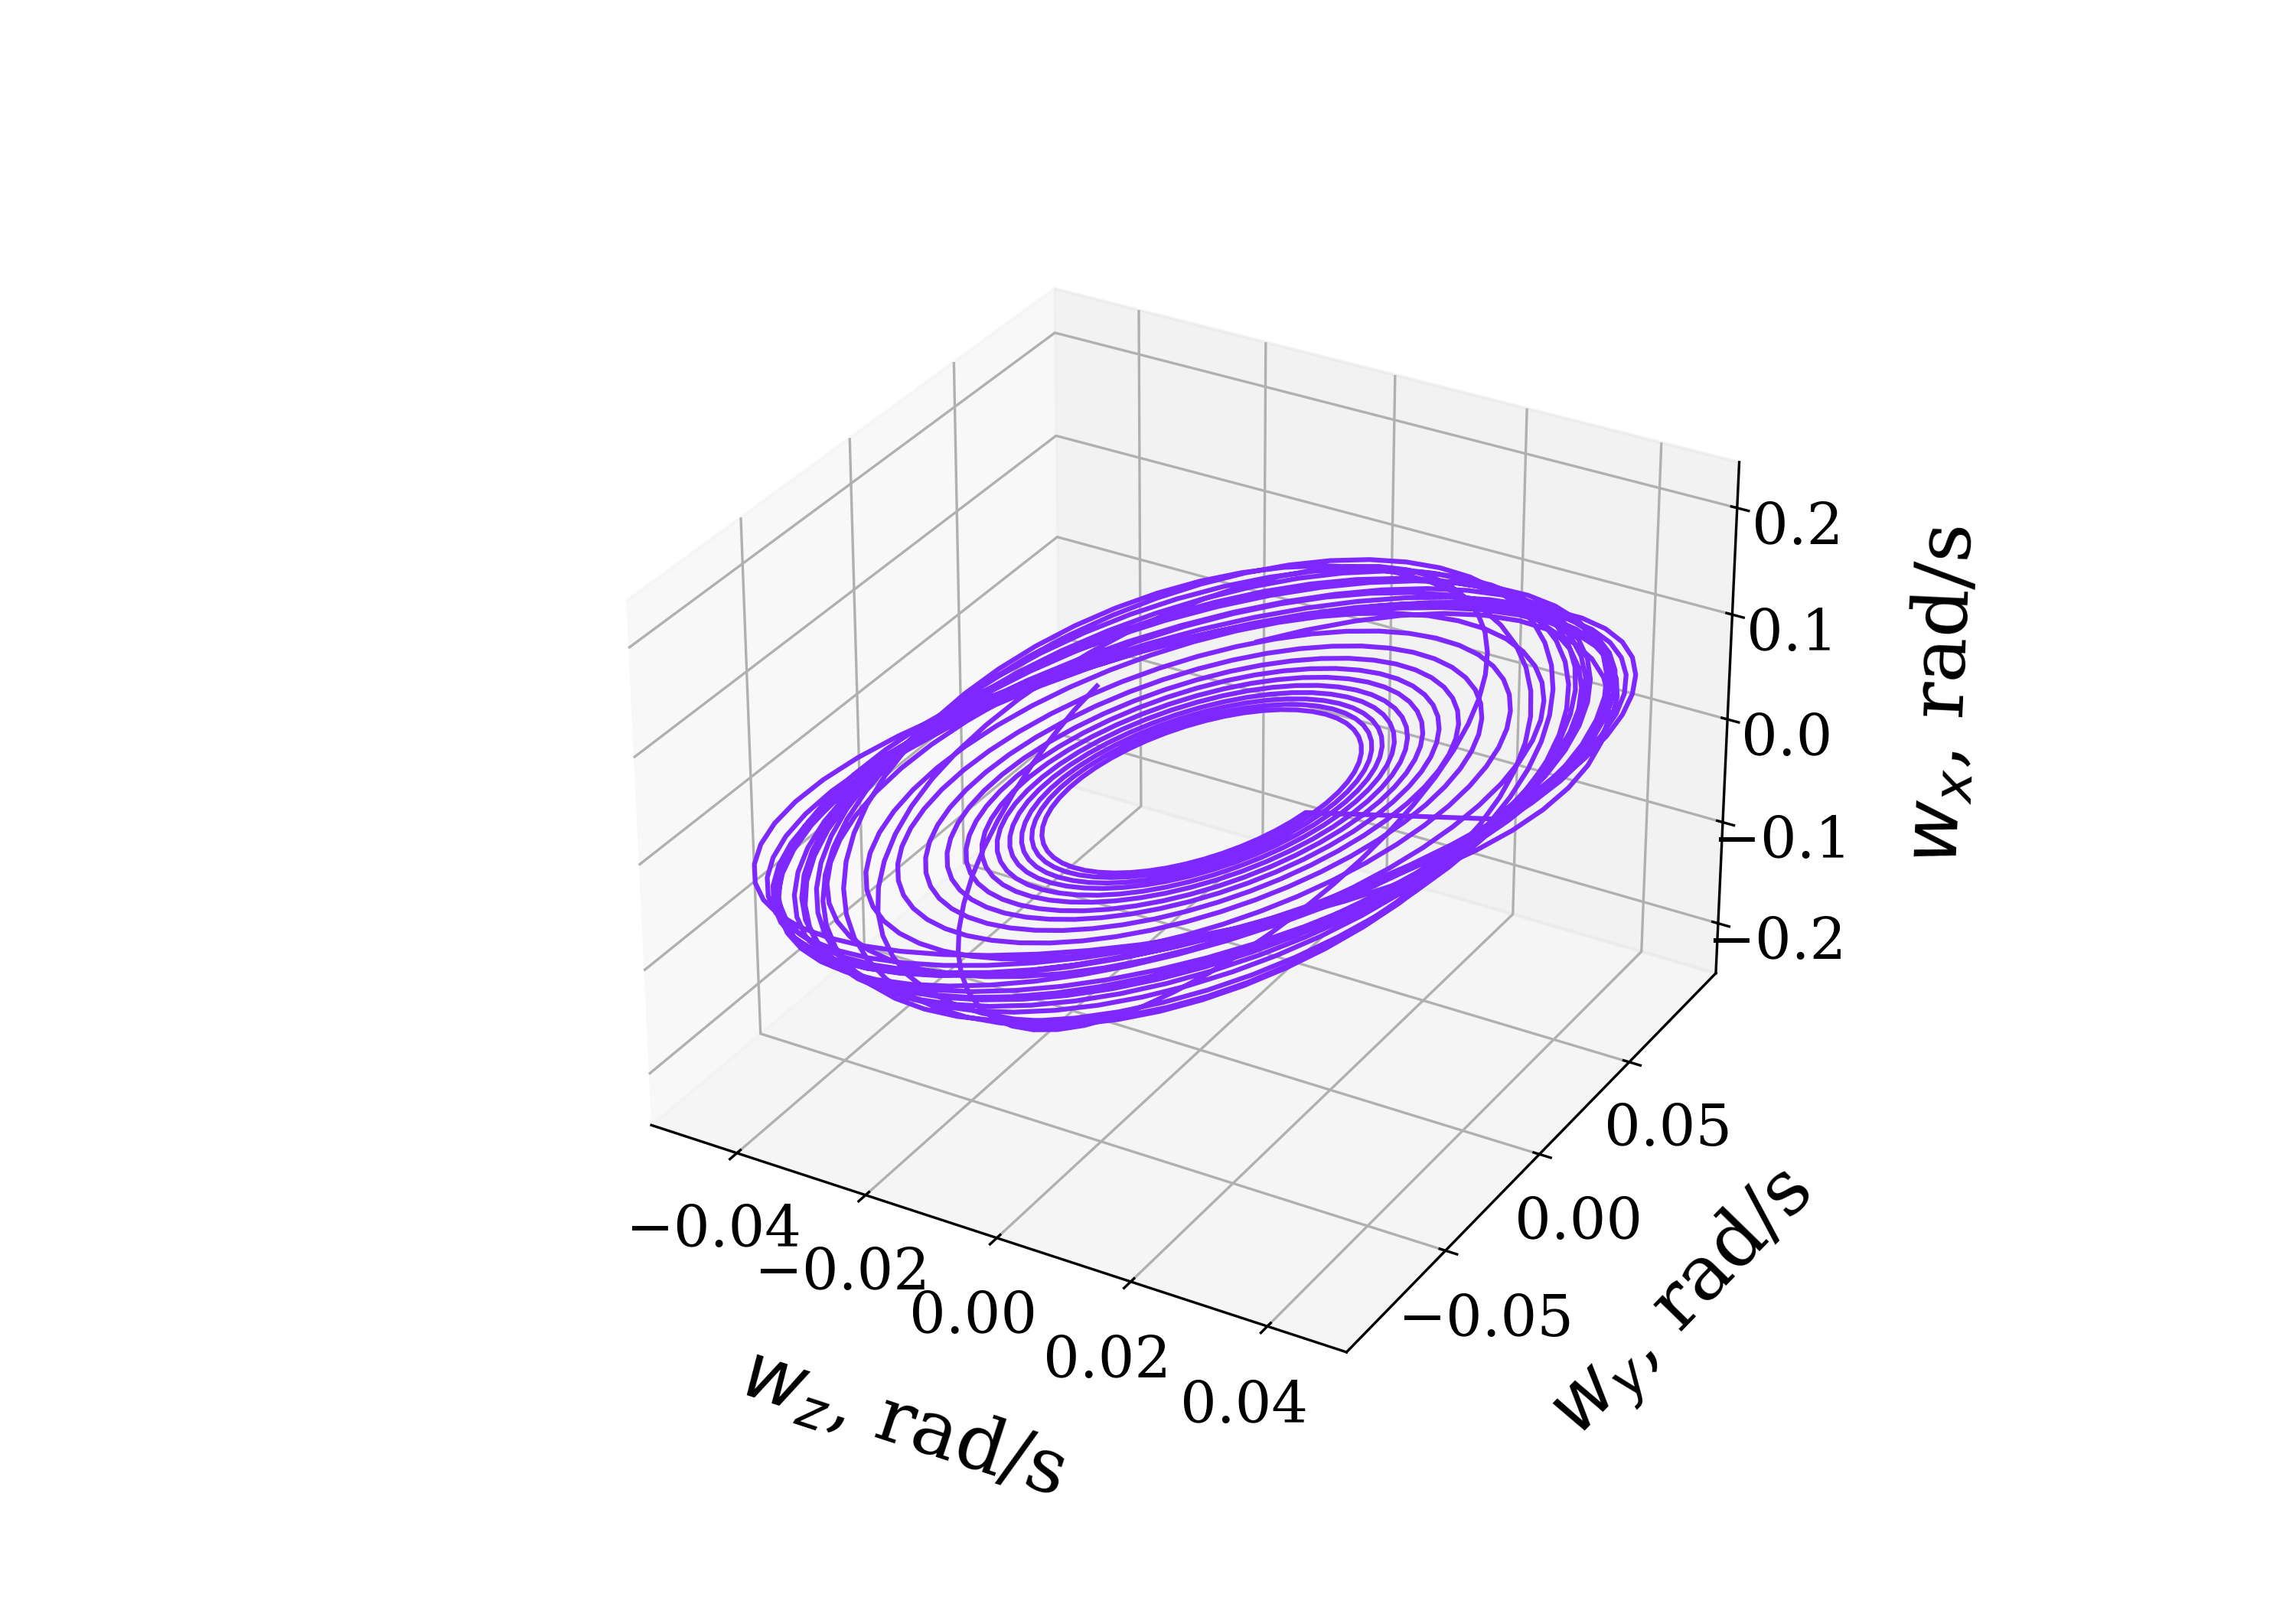
\includegraphics[width=0.48\textwidth, keepaspectratio]{gyro_1_mssa.png}
		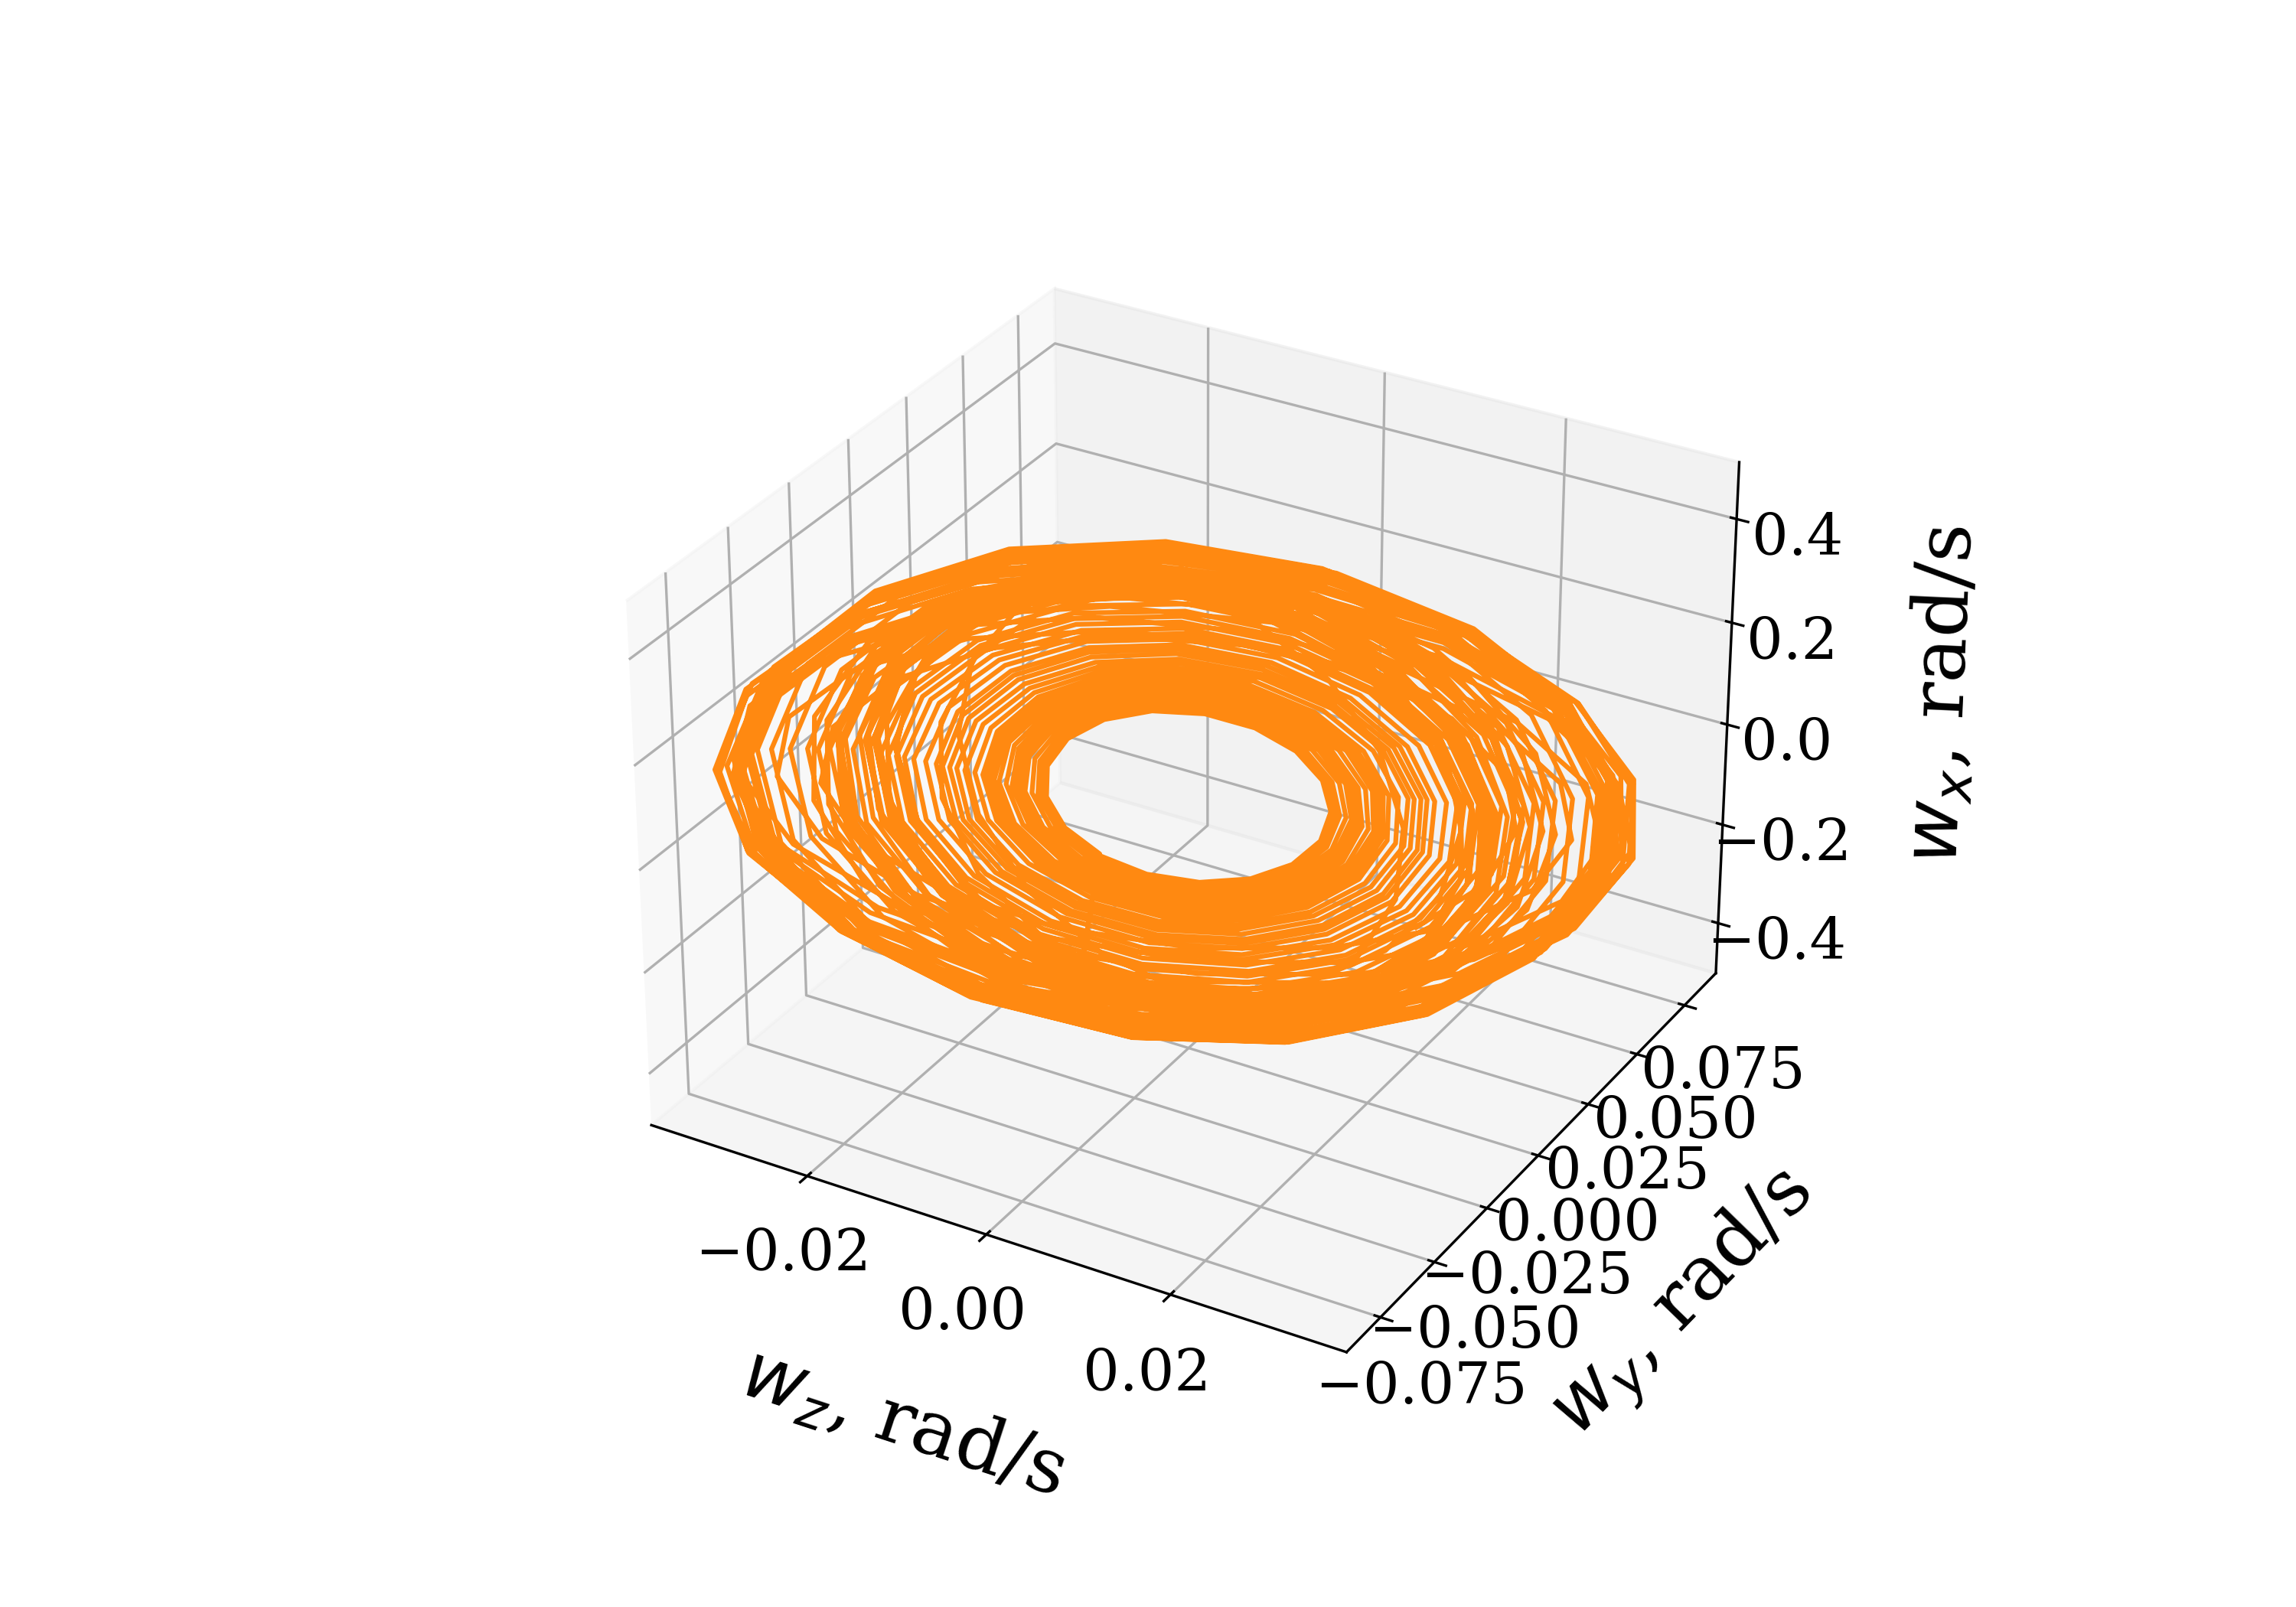
\includegraphics[width=0.48\textwidth, keepaspectratio]{gyro_2_mssa.png}
		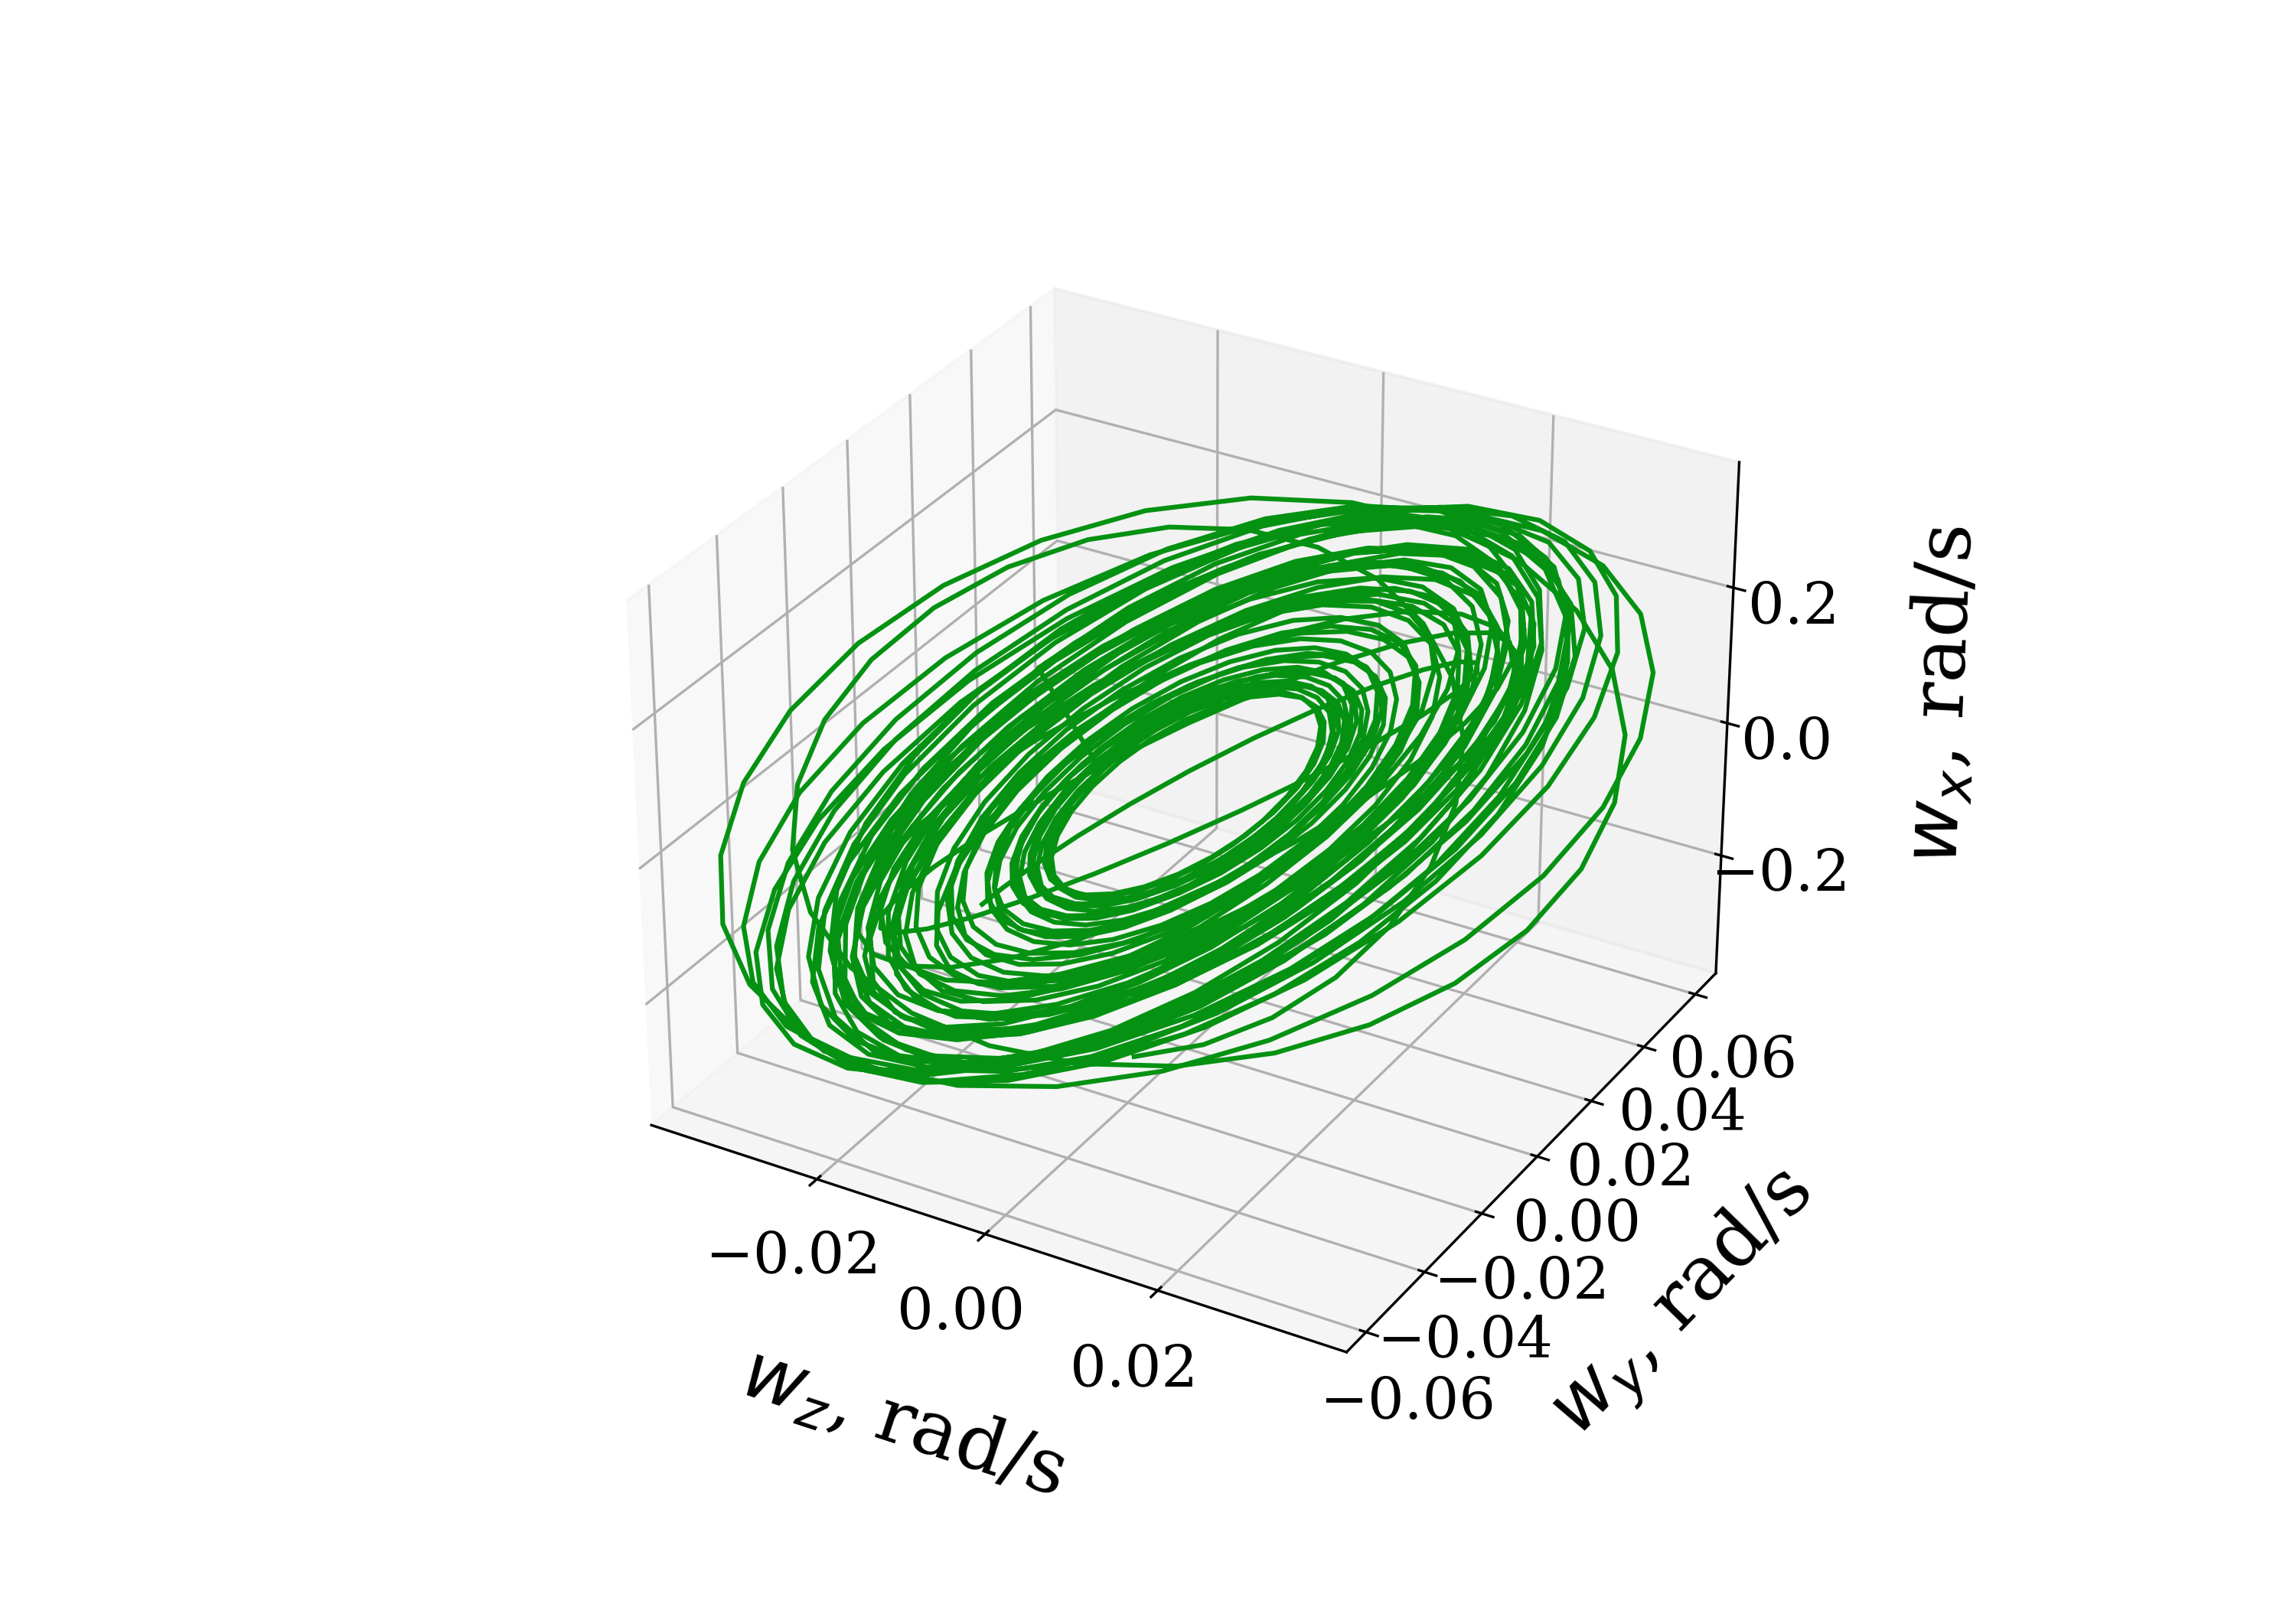
\includegraphics[width=0.48\textwidth, keepaspectratio]{gyro_3_mssa.png}
		\caption{mSSA decomposition for the gyroscope data}\label{fig:gyro_decomp_mssa}
	\end{figure}
	
	\def\arraystretch{1.2}
	\begin{table}[h!]
		\centering
		\caption{Decomposition quality of the models for the electricity data}\label{tab:decomp_electr_results}
		\begin{tabular}{|c|c|c|}
			\hline
			& tSSA  & mSSA           \\ \hline
			$ \overline{\text{RHE}}_{\text{Producution}} $  & 0.507 & 0.308          \\ \hline
			$ \overline{\text{RHE}}_{\text{Price}} $      & 0.511 & 0.31           \\ \hline
			$ \overline{\text{RHE}} $             & 0.509 & \textbf{0.309} \\ \hline
		\end{tabular}
	\end{table}
	
	\def\arraystretch{1.2}
	\begin{table}[h!]
		\centering
		\caption{Decomposition quality of the models for the inertial unit data}\label{tab:decomp_motion_results}
		\begin{tabular}{|c|c|c|}
			\hline
			& tSSA  & mSSA           \\ \hline
			$ \overline{\text{RHE}}_{\text{Accel}} $   & 0.438 & 0.394          \\ \hline
			$ \overline{\text{RHE}}_{\text{Gyro}} $ & 0.732 & 0.468          \\ \hline
			$ \overline{\text{RHE}} $         & 0.585 & \textbf{0.431} \\ \hline
		\end{tabular}
	\end{table}	
	
	\section{Conclusion}
	
		Proposed tensor method is devoted to the forecast and the additive decomposition of the interdependent multivariate time series. It is based on dynamical systems theory and explicitly build the shared phase space of the series. It also exploits multilinearity of the data via tensor data representation. The method has only two adjustable parameters and require the CPD computation of the trajectory tensor. Then, the forecast comes down to the vector's scalar product. The decomposition comes down to matrix factorization and factor's partitioning. Finally, the computational experiment showed tSSA's high forecast and decomposition quality. The method also reduced dimensionality of the given data.
		
		A tSSA's disadvantage is an NP-hardness of the optimal series decomposition. Relaxation of this problem or finding another principle to build additive components are the major directions for further method improvement. Another future research task is the extension of the dynamical systems approach and proposing a new way of building the shared phase space. 
		
		\bibliography{lit}
	
 \end{document}